\documentclass[11pt,twoside,a4paper]{report}

\usepackage[a4paper]{geometry}

\usepackage[brazil]{polyglossia}
\usepackage{lmodern}

%%For XeLaTeX
\usepackage[xetex, draft=false, colorlinks=true, breaklinks=true, bookmarks=true, pdftitle={Creating a HasCASL Library}, pdfauthor={G. M. Cabral and A. V. Moura}]{hyperref}
\usepackage{hypcap}

\usepackage[xetex]{graphicx}

%Fonts
\usepackage{fontspec} % provides font selecting commands 
\usepackage{xunicode} % provides unicode character macros 
\usepackage{xltxtra}  % provides some fixes/extras 
%\defaultfontfeatures{Scale=MatchLowercase,Mapping=tex-text}
%\setmainfont[Mapping=tex-text]{Baskerville}
%\setsansfont[Mapping=tex-text]{Skia} 
%\setmonofont{Courier} 

%For printing - few ink
%\setmainfont{Spranq Eco Sans}
%\setsansfont{Spranq Eco Sans}
%\setmonofont{Andale Mono}

\usepackage{amsmath}

\usepackage{multicol}
\setlength{\columnseprule}{0.1pt}

%Bibliography
\usepackage{natbib}
\setcitestyle{numbers,square}
\bibliographystyle{plainnat}
%\bibliographystyle{abbrvnat}
%\bibliographystyle{unsrtnat}

\usepackage{url}

%For Headers
\usepackage{fancyhdr}
\pagestyle{fancy}

%For double line space
\usepackage{setspace}
%\doublespace

%For Appendix
\usepackage{appendix}

%fancyvrb: for customizable verbatim env.
\usepackage{fancyvrb}
\fvset{fontsize=\relsize{-1}}

%relsize: for font resizing
\usepackage{relsize}

% My macros
% Macro for citing Appendix
\newcommand{\citeAppendix}[1]{Apêndice~\ref{#1}, na página~\pageref{#1}}
%Macro for citing Specification
\newcommand{\citeSpec}[1]{Especificação~\ref{#1}, na página~\pageref{#1}}
%Macro for citing Proof Excerpt
\newcommand{\citeProof}[1]{Excerto de Prova do Isabelle~\ref{#1}, na página~\pageref{#1}}
%Macro for citing Full Proof Excerpt
\newcommand{\citePScript}[1]{Prova do Isabelle~\ref{#1}, na página~\pageref{#1}}
%Macro for citing figure
\newcommand{\citeFig}[1]{Figura~\ref{#1}, na página~\pageref{#1}}
% Macro for referencing axiom
\newcommand{\axiom}[1]{{\tt \%(#1)\%}}
% Macro for referencing Haskell Code
\newcommand{\citeHaskell}[1]{Código-fonte Haskell~\ref{#1}, na página~\pageref{#1}}

\usepackage{xspace}
\newcommand{\HasCASL}{\textsc{HasCasl}\xspace}
\newcommand{\CASL}{\textsc{Casl}\xspace}
\newcommand{\Hets}{\textsc{Hets}\xspace}
\newcommand{\Haskell}{\textsc{Haskell}\xspace}
\newcommand{\ML}{\textsc{ML}\xspace}
\newcommand{\HOL}{\textsc{HOL}\xspace}
\newcommand{\Isabelle}{\textsc{Isabelle}\xspace}
\newcommand{\Prelude}{\textsc{Prelude}\xspace}
\newcommand{\HOLCF}{\textsc{HOLCF}\xspace}
\newcommand{\SML}{\textsc{SML}\xspace}
\newcommand{\EML}{\textsc{EML}\xspace}
\newcommand{\Maude}{\textsc{Maude}\xspace}
\newcommand{\Larch}{\textsc{Larch}\xspace}
\newcommand{\Z}{\textsc{Z}\xspace}

\newcommand{\sort}{tipo (\textit{sort})\xspace}
\newcommand{\sorts}{tipos (\textit{sorts})\xspace}

\newcommand{\kind}{tipo (\textit{kind})\xspace}
\newcommand{\kinds}{tipos (\textit{kinds})\xspace}

\newcommand{\type}{tipo (\textit{type})\xspace}
\newcommand{\types}{tipos (\textit{types})\xspace}

% Está conflitando com as figuras. Não usar!
%%For XeLaTeX, insert xetex option inside hyperref
%\usepackage[xetex, draft=false, colorlinks=true, breaklinks=true, bookmarks=true, pdftitle={Creating a HasCASL Library}, pdfauthor={G. M. Cabral and A. V. Moura}]{hyperref}
%\usepackage[all]{hypcap}



\fancyhead{}
\fancyhead[el]{\thepage}
\fancyhead[er]{\textit{Cabral, G. M.}}
\fancyhead[ol]{\textit{Criação de uma biblioteca padrão para a linguagem \HasCASL}}
\fancyhead[or]{\thepage}
\fancyfoot{}
%\fancyfoot[l]{Rev: \svnrev\ (\svnfilerev)}
%\fancyfoot[r]{\svnyear-\svnmonth-\svnday \hspace{0.5cm} \svnhour:\svnminute} % Date
\renewcommand{\headrulewidth}{0pt}
\renewcommand{\footrulewidth}{0pt}

% Fancy style for chapter page (\maketitle uses plain style):
\fancypagestyle{plain}{%
\fancyhf{}
%\fancyfoot[ol]{Rev: \svnrev\ (\svnfilerev)}
\fancyhead[or]{\thepage}
%\fancyfoot[or]{\svnyear-\svnmonth-\svnday \hspace{0.5cm} \svnhour:\svnminute} % Date
\renewcommand{\headrulewidth}{0pt}
\renewcommand{\footrulewidth}{0pt}
}

\title{\textbf{Relatório Final de Mestrado}\\
\ \\
Criação de uma biblioteca padrão para a linguagem \HasCASL}

\author{Glauber Módolo Cabral\thanks{Instituto  de Computação, Universidade Estadual  de Campinas, 13081-970  Campinas,  SP.  Suporte CNPq Processo: 132039/2007-9}}

\date{Processo CNPq: 132039/2007-9\\
\ \\
Período de Fomento: Março de 2007 a Fevereiro de 2009\\
\ \\
Previsão de Defesa: Fevereiro de 2010}

\begin{document}

\maketitle

\begin{abstract}
Este relatório contém uma versão preliminar da dissertação de mestrado do aluno \textit{Glauber Módolo Cabral}, desenvolvida sob a orientação do professor \textit{Dr. Arnaldo Vieira Moura}, no programa de \textit{Mestrado Acadêmico} da \textit{Universidade Estadual de Campinas (UNICAMP)}.
O trabalho consistiu em especificar uma biblioteca para a linguagem de especificação algébrica \HasCASL tendo como ponto de partida a biblioteca \Prelude da linguagem de programação \Haskell.
Aqui, relatamos as dificuldades encontradas durante o trabalho, bem como os resultados obtidos com a execução do mesmo e  apresentamos algumas propostas de trabalhos.
\end{abstract}

\setcounter{page}{1}
\pagenumbering{roman}
\tableofcontents 
\newpage
\pagenumbering{arabic}
\setcounter{page}{1}


\chapter{Sumário Executivo}
\label{chap:sumario}

O presente relatório apresenta uma versão preliminar da dissertação de mestrado do aluno \textit{Glauber Módolo Cabral}, desenvolvida sob a orientação do professor \textit{Dr. Arnaldo Vieira Moura}, no programa de \textit{Mestrado Acadêmico} da \textit{Universidade Estadual de Campinas (UNICAMP)}.
Este trabalho está inserido no âmbito do processo CNPq n$\,^{\circ}$: 132039/2007-9.

O projeto original contemplou a construção de uma biblioteca para a linguagem de especificação algébrica \HasCASL.
A especificação teve como base a biblioteca \Prelude pertencente à linguagem de programação \Haskell.
O texto detalha as decisões técnicas e discute detalhes da especificação desenvolvida.

A fim de representar totalmente os recursos da linguagem \Haskell, a biblioteca deveria utilizar avaliação preguiçosa de dados, funções contínuas e tipos de dados infinitos.
Para tanto, seria necessário fazer uso das construções mais avançadas da linguagem \HasCASL, cujas provas envolveriam duas lógicas no provador de teoremas \Isabelle e exigiriam algumas opções do analisador sintático e tradutor de códigos \Hets que ainda não haviam sido implementadas à época do início do trabalho.
Em face destes fatos, optou-se por utilizar a avaliação estrita de tipos de dados na biblioteca e deixar a introdução de recursos mais avançados para um refinamento posterior.

%Dificuldades
A primeira dificuldade encontrada envolveu as linguagens \CASL e \HasCASL.
Embora ambas possam ser usadas conjuntamente, uma vez que todas as construções de \CASL são válidas na linguagem \HasCASL, existem algumas exceções.
Por outro lado, nosso plano original previa apenas utilizar a linguagem \HasCASL e seus recursos.
O manual então existente descrevia apenas a linguagem \CASL e suas aplicações.
A documentação da linguagem \HasCASL ainda está voltada para questões teóricas envolvidas nas construções da linguagem e não descreve facilmente o uso destas últimas.
Dessa forma, usar precisamente a sintaxe de ambas as linguagens, uma vez que a quase totalidade de exemplos existentes estão escritos em \CASL, mostrou-se uma tarefa complexa.

Uma outra dificuldade no início do trabalho envolveu a correta diferenciação entre as relações lógicas (igualdade e relações de ordem) da linguagem \HasCASL e as funções presentes na biblioteca para as mesmas relações lógicas.
Como o tipo \Verb.Bool. foi redefinido, a equivalência lógica entre axiomas causou certa confusão.
Embora os axiomas fossem equivalentes, o uso dos mesmos como regras de reescrita pelo provador de teoremas não era equivalente.
Mais especificamente, axiomas podiam ser definidos por igualdade, como em
\begin{Verbatim}
. (x > y) = (y < x)
\end{Verbatim}

ou pelo operador de equivalência de \HasCASL, como em
\begin{Verbatim}
. (x > y) = True  <=> (y < x) = True
\end{Verbatim}

No primeiro caso, embora fosse uma melhor escolha como regra de reescrita, não foi possível associar um valor do tipo \Verb.Bool. redefinido a cada membro da igualdade.
O segundo caso, embora adicione informações aparentemente redundantes, representa a forma correta de definir uma regra de reescrita com o tipo \Verb.Bool. redefinido.
A fim de implementar a primeira sintaxe, permitindo maior clareza no código, foi necessário realizar a introdução da avaliação preguiçosa e a alteração do tipo de dados \Verb.Bool..

O aprendizado do uso do provador de teoremas \Isabelle também se mostrou um fator complicador considerável no trabalho.
A decisão de escrever as provas usando a linguagem \HOL ao invés de \textit{Isar}, embora tenha simplificado o início do trabalho por ser a linguagem utilizada no tutorial do provador, tornou a escrita de provas maiores um trabalho mais complexo.
Um detalhe que causou certa dificuldade inicial foi a maneira como \Isabelle usa os axiomas como regras de reescrita.
Se um predicado \Verb.P. implica em um predicado \Verb.Q. (\Verb.P ==> Q.), o provador de teoremas tenta casar o predicado \Verb.Q. com o alvo a ser provado, construindo a prova de baixo para cima, o que não é a forma usual de se raciocinar.

Como \HasCASL é um projeto em desenvolvimento, a ferramenta \Hets, para análise e tradução de especificações, não está completamente implementada.
Especificações envolvendo avaliação preguiçosa e o subconjunto executável da linguagem \HasCASL ainda não podem ser traduzidos para uso direto no provador de teoremas \Isabelle.
As dificuldades foram sanadas graças a soluções gentilmente sugeridas pelos desenvolvedores da ferramenta \Hets.

%Resultados principais
O trabalho resultou em uma biblioteca que inclui a especificação de quase todos os tipos de dados e de várias funções presentes na biblioteca \Prelude.
Foi utilizada a avaliação estrita de tipos de dados ao invés da avaliação preguiçosa devido à complexidade que esta última introduz nas especificações e ao fato de a avaliação preguiçosa poder ser introduzida na biblioteca através de um futuro refinamento.
A quase totalidade dos teoremas propostos para as especificações da biblioteca foi provada através do provador de teoremas \Isabelle.

Em um segundo momento do trabalho foi realizada uma extensão da biblioteca para adicionar o uso da avaliação preguiçosa de tipos de dados.
Esta extensão resultou em uma nova versão da biblioteca e na necessidade de se reescrever as provas desenvolvidas.
Embora essa extensão ainda não tenha traduzido a biblioteca para o subconjunto executável da linguagem \HasCASL, que pode ser traduzido para a linguagem de programação \Haskell, a biblioteca pode ser usada para especificar pequenos programas envolvendo tipos básicos de dados e estruturas simples.

%Trabalhos Futuros
O trabalho ainda apresenta algumas provas incompletas e algumas funções da biblioteca \Prelude ainda sem especificação.
Algumas das provas parecem requerer conhecimentos avançados da linguagem \HOL e as funções não especificadas envolvem algumas questões em aberto.

Uma das questões que permanece em aberto é o tratamento de especificações numéricas, as quais não conseguem ser usadas pelo provador \Isabelle como regras de reescrita justamente por não possuírem todos os lemas correlatos necessários e nem vínculos entre seus axiomas e axiomas dos tipos numéricos presentes na linguagem \HOL.
Especificar todos os tipos numéricos novamente para incluir os lemas faltantes não se mostrou uma opção viável.
Uma possível solução seria criar isomorfismos entre os tipos numéricos da linguagem \HOL e os tipos especificados nas bibliotecas numéricas da linguagem \CASL.
Se o isomorfismo for chamado de \Verb.h., pode-se provar um alvo da forma \Verb.t1 = t2. injetando o isomorfismo através da regra \Verb.h x = h y ==> x = y..
Esta regra resulta em um novo alvo, \Verb.h t1 = h t2., que poderia ser escrito em termos de tipos primitivos de \HOL e, dessa forma, ser provado pelo provador \Isabelle com os axiomas e lemas preexistentes em \HOL.
Este isomorfismo poderia ser estendido para a especificação de listas.
Como a linguagem \Haskell trabalha basicamente com listas, esta extensão do isomorfismo facilitaria o processo de prova de várias especificações.

Uma solução para o problema dos tipos numéricos permitiria que o restante das funções da biblioteca \Prelude pudessem ser especificadas e verificadas.
É o caso, por exemplo, de várias funções da especificação \Verb.List. que foram suprimidas uma vez que a sua inclusão, devido a dependência de especificações numéricas, impedia a construção das provas de lemas envolvendo as demais funções não dependentes de números.

Embora tenha sido realizada a inclusão inicial da avaliação preguiçosa, ainda é necessário utilizar o subconjunto executável da linguagem \HasCASL para que o comportamento das especificações seja equivalente ao das funções em \Haskell.
No entanto, o uso deste subconjunto já permitiria a especificação de recursão e de tipos infinitos de dados, bem como a tradução das especificações para códigos executáveis em \Haskell.

% Descrição do documento
\setstretch{0.9}
As demais seções estão organizadas da seguinte forma.
A Seção \ref{chap:revisaobib} apresenta um breve resumo de algumas linguagens de especificação formal existentes, e que são relacionadas à linguagem utilizada neste trabalho.
A Seção \ref{chap:HasCASLTutorial} introduz a linguagem de especificação algébrica \CASL e descreve em maiores detalhes a linguagem \HasCASL, a sublinguagem de \CASL utilizada neste trabalho e que possui suporte para lógica de segunda ordem e, também, um subconjunto de construções semânticas semelhantes à linguagem de programação \Haskell.
A construção da biblioteca que foi objeto de estudo está relatada na Seção \ref{chap:desenvBiblioteca}, justificando decisões de projeto e detalhando as especificações criadas.
A verificação da biblioteca criada na seção anterior é reportada na Seção \ref{chap:hetseisabelle}, introduzindo as ferramentas necessárias para a verificação e explicando seu uso na verificação da biblioteca desenvolvida.
Como a biblioteca criada não contemplou o uso de avaliação preguiçosa, recursão e tipos de dados infinitos, uma extensão da biblioteca foi realizada com o intuito de incluir suporte a estes elementos. A Seção \ref{chap:laziness} descreve esta extensão, discutindo o que foi realizado e os problemas que ainda persistem.
Os Apêndices \ref{appendix:strictSpec} e \ref{appendix:strictProofs} listam, respectivamente, o código da biblioteca na versão sem avaliação preguiçosa e as provas escritas para esta versão da biblioteca. A biblioteca resultante da extensão está listada no Apêndice \ref{appendix:lazySpec} e as respectivas provas encontram-se no Apêndice \ref{appendix:lazyProofs}.

\setstretch{1}
\chapter{Linguagens de Especificação Formal Correlatas}
\label{chap:revisaobib}

Neste capítulo, realizamos uma compilação de natureza ilustrativa e introdutória de algumas linguagens de especificação formal disponíveis.
Sem a pretensão de extensão ou de completude, as seções a seguir visam a uma apresentação das características de linguagens de especificação formal.
Para uma visão aprofundada, deve-se consultar as referências assinaladas em cada seção.

\section{Extended ML}\label{chap:revisaobib:eml}
\textit{Extended ML (\EML)} \cite{MLDefIntro} é em uma linguagem formal que foi construída a partir da linguagem de programação funcional \textit{Standard ML (\SML)}, estendendo a sintaxe e a semântica desta última para alcançar o formalismo necessário para a execução de inferências lógicas.

A linguagem de programação funcional \textit{Standard ML (\SML)} é composta por duas sublinguagens.
A primeira, nomeada linguagem \textit{core}, provê a definição de tipos e valores (variáveis, funções e elementos) daqueles tipos.
A segunda, chamada linguagem \textit{module}, permite a definição e a combinação de unidades autocontidas de programas codificadas na primeira linguagem.

A linguagem \textit{core} é uma linguagem fortemente tipificada com um sistema de tipos que agrega tipos polimórficos, união disjunta de tipos, produtos de tipos, tipos que são funções de segunda ordem, tipos recursivos e a possibilidades de definição de tipos abstratos e concretos pelo usuário.
A semântica da linguagem também reflete características de linguagens imperativas de programação, a saber: tratamento de exceções e referências (ponteiros) tipificadas.
O tratamento de entrada e saída de dados é realizado através de \textit{streams}, que associam o fluxo de entrada com produtores (teclado, por exemplo) e o fluxo de saída com consumidores (monitor).

A linguagem \textit{module} fornece mecanismos para a modularização de programas.
Uma assinatura (\textit{signature}) fornece uma interface que é implementada por uma estrutura (\textit{structure}).
Nesta interface são declarados tipos, valores, exceções e subestruturas que devem ser implementados pelas estruturas posteriormente associadas a esta assinatura.
A linguagem ainda apresenta funtores, equivalentes a estruturas parametrizadas, que são aplicados sobre outras estruturas a fim de se obter novas estruturas.
Um funtor possui uma assinatura de entrada, que descreve as estruturas às quais pode ser aplicado, e uma assinatura opcional de saída, que define a estrutura resultante da aplicação do mesmo sobre outras estruturas.
Estruturas e funtores definem módulos e as assinaturas, por sua vez, impõem restrições às definições de módulos, além de definirem quais declarações dos módulos serão visíveis pelos usuários destes módulos.

Além de ter sua sintaxe e sua semântica formalmente definidas, a linguagem \SML possui uma biblioteca padrão definida e que deve ser implementada pelos compiladores \cite{MLLib}.
A biblioteca especifica interfaces e operações para tipos básicos de dados, como inteiros, caracteres e cadeias de caracteres, listas, tipos opcionais e vetores mutáveis e imutáveis.
Também são definidos o suporte para operações de entrada e saída binária e textual, além de interfaces para serviços do sistema operacional e para comunicação em rede.

A linguagem \EML permite o desenvolvimento formal de programas através de passos individualmente verificados.
Ela engloba todos os estágios deste desenvolvimento, desde a especificação de alto nível até o programa final.
Por ter como produto final um programa modular escrito na linguagem \SML, um grande subconjunto desta última linguagem forma uma sublinguagem executável de \EML.

Além das características pertencentes às linguagens de programação funcional, \EML possui outras duas características particularmente interessantes para a aplicação em métodos formais.
Primeiramente, permite total modularização para a modelagem de sistemas complexos.
A modularização é um pré-requisito para a aplicação de métodos formais no desenvolvimento de exemplos complexos e \EML foi projetada visando ao seu emprego neste contexto.
Em segundo, a sintaxe e a semântica da linguagem são formalmente definidas.
Com a definição formal, torna-se possível fazer inferências por meio de lógica formal sobre o comportamento de programas escritos em \SML, o que permite, por sua vez, o desenvolvimento de provas de correção segundo uma dada especificação formal.

\EML foi desenvolvida com o propósito de ser uma extensão mínima à linguagem \SML.
Tem como princípio o desenvolvimento de uma linguagem para especificar sistemas modulares escritos em \SML ao invés do desenvolvimento de uma linguagem de especificação de propósito geral.
Devido a essa abordagem, \EML pode ser facilmente aprendida por aqueles que possuem contato anterior com \SML.
No entanto, devido à complexidade da linguagem \SML, a sintaxe de \EML também é complexa e seu manuseio no processo de especificação e verificação torna-se difícil.
Uma outra desvantagem da linguagem é a falta de suporte a ferramentas automáticas de verificação, tais como provadores de teoremas \cite{MLSurvay}.

A principal extensão de \EML com relação à sintaxe de \SML é a inclusão de axiomas nas assinaturas e no corpo dos módulos.
Os axiomas definem propriedades que devem ser satisfeitas por todas as estruturas que implementarem a interface onde eles foram definidos.
Assim como os tipos dos valores definidos nas interfaces de \SML permitem com que cada módulo seja compilado separadamente, a inclusão de axiomas nas interfaces de \EML permite com que propriedades dos módulos descritos por uma interface possam ser verificadas sem que seja necessário verificar o conteúdo do módulo.
Isto cria a facilidade para que implementações diferentes de uma mesma interface sejam criadas e possam ser utilizadas sem afetar a correção das provas anteriormente desenvolvidas.

Ao contrário de \SML, em que é opcional a definição de assinaturas para estruturas, todas as estruturas definidas em \EML devem possuir, obrigatoriamente, uma assinatura.
No caso dos funtores, ambas as assinaturas de entrada e saída se tornam obrigatórias.
Além do casamento entre nomes e tipos entre as entidades de uma assinatura e de um módulo, o corpo do módulo deve estar correto, ou seja, deve satisfazer todos os axiomas da assinatura a que está associado.

Uma terceira extensão permite que o desenvolvimento de um programa em \EML comece com a definição de módulos de forma abstrata.
Pode-se utilizar um sinal de interrogação no lugar da definição do corpo de um módulo, permitindo que sua definição seja incluída em refinamentos posteriores.
Axiomas definindo o comportamento esperado da estrutura com declaração abstrata são declarados logo em seguida.
Nos refinamentos posteriores, o sinal de interrogação é substituído por código escrito em \SML, o qual deve obedecer às propriedades definidas pelos axiomas.
O desenvolvimento em \EML é encerrado quando todos os sinais de interrogação são substituídos por código \SML executável e os axiomas transformados em documentação.

\EML possui um analisador sintático para verificar especificações e o código \SML resultante do processo de especificação pode ser analisado e gerado pelo compilador da linguagem \SML.
No entanto, a linguagem ainda não possui ferramentas de verificação formal associadas, tal como um provador de teoremas ou um verificador automático de propriedades.
A linguagem também não possui uma biblioteca padrão, embora tenha algumas funções pré-definidas na linguagem, tais como: tipo booleano e operações lógicas, listas e operações associadas, números (inteiros e reais) e funções aritméticas, cadeias de caracteres e operações de concatenação e quebra de cadeias \cite{MLDef}.

\section{Maude}\label{chap:revisaobib:maude}

A linguagem de especificação formal \Maude \cite{MaudeBook} foi projetada sobre três pilares: simplicidade, expressividade e performance.
Dessa forma, uma grande variedade de aplicações deveriam ser naturalmente modeláveis na linguagem, de forma simples e com significado claro, e as implementações concretas destas aplicações deveriam ter performance competitiva com outras linguagens de programação eficientes.

Um programa \Maude pode ser escrito através de equações e de regras, as quais possuem uma semântica de reescrita simples na qual o padrão encontrado do lado esquerdo é substituído pelo lado direito da equação ou da regra correspondente.

Se um programa \Maude contem apenas equações, ele é considerado um \textit{módulo funcional}.
Este módulo é um programa funcional onde são definidas, através de equações, uma ou mais funções que serão utilizadas como regras de simplificação.
As equações podem, também, ser equações condicionais, ou seja, sua aplicação pode depender da validade de uma condição.
Os módulos funcionais permitem definir sistemas determinísticos.

Um programa que contem regras e, opcionalmente, equações, é considerado um \textit{módulo de sistema}.
Assim como equações, as regras também são tratadas por reescrita do termo à esquerda pelo equivalente à direita e podem, opcionalmente, serem condicionais.
No entanto, as regras diferem de equações por serem consideradas regras de transição local em um sistema possivelmente concorrente.
O sistema pode ser encarado como um multiconjunto de objetos e mensagens, no qual estes últimos interagem localmente entre si através de regras e onde a ordem na qual objetos e mensagens são dispostos dentro do sistema é irrelevante, uma vez que o operador de união de multiconjuntos é declarado com as propriedades de associatividade e comutatividade.
Um sistema declarado desta forma pode ser altamente concorrente e não-determinístico, ou seja, não há garantias de que todas as sequências de reescrita levam a um mesmo resultado final.
Dependendo da ordem em que as regras forem aplicadas, os objetos podem terminar em estados diferentes, uma vez que as regras condicionais poderão, ou não, ser aplicadas devido ao estado dos objetos, nos diferentes caminhos possíveis de aplicação de mensagens, satisfazerem, ou não, as condições das regras.
Há, ainda, a possibilidade de que não haja um estado final, ou seja, mensagens e objetos podem permanecer em interação contínua, formando um sistema reativo.

A linguagem \Maude, além de permitir a definição de sistemas determinísticos e não-determinísticos, ainda é capaz de lidar com casamento de padrões em equações, definição de sintaxe e tipos de dados pelo usuário, polimorfismo --- com tipos, subtipos e funções parciais ---, tipos e módulos genéricos  --- podendo ser parametrizados por tipos e por novas teorias ---, objetos --- suportando orientação a objetos e comunicação através de mensagens com objetos externos ao sistema (arquivos, 
\textit{socket} de rede, banco da dados, etc) --- e reflexão --- suportando redefinição de estratégias de reescrita, extensão dos módulos com novas operações e permitindo análises e transformações executadas por ferramentas de verificação.

A boa performance dos programas \Maude provem da pré-compilação dos códigos para autômatos de casamento de padrões e de substituição eficientes.
Esta pré-compilação permite, ainda, armazenar e analisar todos os passos de reescrita realizados.
Ainda é possível otimizar o código através de outras quatro ferramentas.
A ferramenta Perfil permite analisar gargalos de execução.
As Estratégias de Avaliação permitem indicar quais argumentos devem ser avaliados e em qual ordem, antes que sejam executadas simplificações com equações, permitindo avaliação preguiçosa, avaliação estrita ou algum tipo de avaliação entre as duas anteriores.
É possível, também, congelar a posição de argumentos em regras, evitando que estas últimas sejam aplicadas em qualquer subtermo naquela posição.
Por último, é possível sinalizar que o resultado da chamada de funções sobre um determinado operador deve ser guardado para uso posterior, melhorando o tempo de execução de determinadas funções.

A linguagem \Maude pode ser usada com três finalidades.
Sistemas podem ser diretamente programados em \Maude, tirando vantagem da simplicidade da linguagem e das suas características formais.
Pode-se, também, modelar um sistema através de uma especificação formal executável, permitindo o uso da especificação como um protótipo preciso do sistema para simular o seu comportamento.
Dependendo do nível de detalhamento e da eficiência exigida, a especificação já pode ser considerada o programa final ou o modelo pode ser implementado em alguma outra linguagem de programação.
As especificações servem, ainda, como modelos que podem ser formalmente verificados com respeito a diferentes propriedades que expressam requisitos formais do sistema.

Propriedades podem ser descritas por fórmulas em lógica de primeira ordem ou em lógica temporal ou podem ser descritas por equações não-executáveis, regras e sentenças de pertinência escritas nas lógicas dos módulos funcionais ou dos módulos de sistema.
As propriedades descritas em lógica de primeira ordem podem ser verificadas através de um provador de teoremas indutivo existente.
As propriedades temporais, por sua vez, podem ser verificadas através do verificador de modelos para lógica temporal linear.
Além de poder definir e verificar propriedades gerais com as duas ferramentas anteriores, \Maude apresenta algumas ferramentas para propriedades específicas.
Módulos funcionais podem ter a sua terminação verificada.
É possível verificar se módulos sem equações condicionais possuem a propriedade de \textit{Church-Rosser} e se são módulos coerentes.
Pode-se, também, verificar se funções foram totalmente definidas em termos dos construtores dos tipos aos que as mesmas se aplicam.
Há, ainda, uma ferramenta específica para simular sistemas de tempo real e realizar verificação de modelos sobre propriedades destes sistemas descritas em lógica temporal.

Além das ferramentas, a linguagem \Maude provê uma biblioteca contendo a especificação do tipo booleano, dos números naturais, inteiros, racionais e de ponto flutuante, além de cadeias de caracteres. A biblioteca ainda possui a especificação de estruturas genéricas de armazenamento, a saber: listas, conjuntos, mapas e vetores.

% Procurar um exemplo de pilha de inteiros

\section{Larch}\label{chap:revisaobib:larch}

\Larch \cite{LarchBook} constitui uma família de linguagens de especificação formal que dá suporte a especificações em duas camadas.
As especificações possuem componentes escritos em duas linguagens: uma linguagem genérica, independente da linguagem de programação na qual pretende-se implementar a especificação, e uma segunda linguagem, dependente da linguagem de programação a ser utilizada posteriormente.
A primeira linguagem recebe o nome de \textit{Larch Shared Language (LSL)} e as linguagens do segundo tipo são genericamente chamadas de \textit{Larch interface languages} --- referenciadas neste texto como linguagens de interface ---, embora cada uma possua seu respectivo nome.

As linguagens de interface são usadas para definir uma camada de comunicação entre componentes de programas, fornecendo as informações necessárias para o uso de cada um destes componentes.
Estas linguagens fornecem uma maneira de definir assertivas em relação aos estados que um programa pode assumir e incorporam notações das linguagens de programação para efeitos colaterais, tratamento de exceções, iteração e concorrência.
A complexidade de cada uma das linguagens depende, diretamente, da complexidade da linguagem de programação associada.

Como os mecanismos de comunicação entre elementos de um programa variam entre as linguagens de programação, o uso de duas camadas de abstração permite que as linguagens de interface sejam modeladas de forma a se aproximar das linguagens de programação associadas.
Por refletirem o comportamento da linguagem de programação, as linguagens de interface evitam o tratamento genérico de questões associadas à semântica da linguagem de programação, tal como o modelo de alocação de memória para variáveis e a forma como parâmetros são passados para funções, por exemplo.
Em comparação com o uso de uma única linguagem de interface genérica para diferentes linguagens e paradigmas, o uso de linguagens especializadas para cada linguagem de programação simplifica o processo de modelagem, tornando as especificações menores e mais claras com respeito à maneira como deverão ser implementadas.

Existem linguagens de interface para as linguagens de programação C, Modula-3, Ada, C++, ML e Smaltalk.
Há, também, uma linguagem genérica que pode ser especializada para outras linguagens de programação ou pode ser utilizada para especificar programas escritos em mais de uma linguagem.
Por encorajar um estilo de programação que enfatiza o uso de abstrações, as linguagens de interface possuem mecanismos para especificar tipos abstratos de dados.
Quando a linguagem de programação associada suporta tipos abstratos de dados, a linguagem de interface é modelada para refletir esta facilidade.
No caso de linguagens de programação que não possuem suporte nativo para tipos abstratos de dados, os tipos abstratos da linguagem de interface são mapeados para entidades equivalentes na linguagem de programação.

Em \Larch, encoraja-se a separação de interesses entre as duas camadas de linguagens.
As especificações nas linguagens de interface devem concentrar detalhes de programação, tais como procedimentos para manipulação de dados e tratamento de exceções, enquanto as especificações descritas em \textit{LSL} devem definir estruturas primitivas a serem usadas pelas demais linguagens.
Esta separação concentra a complexidade das especificações na linguagem \textit{LSL} com as vantagens de melhorar o reuso -- já que esta linguagem não depende da linguagem de programação --, de evitar erros -- uma vez que a semântica desta linguagem é mais simples do que a das linguagens de interface e linguagens de programação relacionadas -- e de facilitar a verificação de propriedades das especificações -- dado que este processo é mais fácil em \textit{LSL}.

As linguagens da família \Larch definem dois tipos de símbolos: operadores e tipos.
Na linguagem \textit{LSL}, operadores são funções totais entre tuplas de valores e um valor de resultado e tipos são conjuntos disjuntos e não-vazios de valores que indicam o domínio e a imagem dos operadores.
Em cada linguagem de interface, ambos os símbolos devem possuir o mesmo significado que possuem na linguagem de programação associada.

A unidade básica de especificação em \textit{LSL} recebe o nome de \textit{trait}.
Esta unidade introduz operadores e suas propriedades, sendo possível, também, definir tipos abstratos de dados.
As propriedades de operadores são definidas através de assertivas, que são equações relacionando operadores e variáveis.
Há, também, a possibilidade de se criar assertivas não equacionais a fim de gerar teorias mais fortes.

A teoria associada a um \textit{trait} é um conjunto infinito de fórmulas em lógica de primeira ordem multisortida, com igualdade, formado exclusivamente por todas as sentenças lógicas que seguem das assertivas definidas no \textit{trait}.
Esta teoria contém igualdades e desigualdades que podem ser provadas por substituição entre termos associados entre si através de igualdades.

Como boa prática, é sugerido que os \textit{traits} definam um conjunto de operadores e propriedades que, embora relacionados, não caracterizem totalmente um tipo específico.
Desta forma, pode-se reutilizar tais operadores e suas propriedades em outros tipos de dados.

As especificações escritas nas linguagens de interface fornecem informações para o uso de uma interface e, também, informações de como implementá-la.
Cada linguagem de interface possui um modelo do estado manipulado pela linguagem de programação associada.
O estado é o mapeamento entre uma unidade abstrata de armazenamento (chamadas \textit{loc}) e um valor.
Toda variável possui um tipo e está associada a uma \textit{loc} deste tipo.
A \textit{loc} pode armazenar apenas valores do seu tipo a qualquer momento.
Os tipos de valores armazenados nas \textit{locs} podem ser valores básicos (constantes, tais como inteiros e caracteres), tipos expostos (estruturas de dados totalmente descritas pelos construtores de tipo da linguagem de programação associada e que são visíveis pelos clientes da interface) e tipos abstratos (estruturas de dados cujas implementações não estão visíveis para o cliente da interface).

Cada linguagem de interface provê operadores aplicáveis às \textit{locs} a fim de se obter seus valores em estados específicos (geralmente, os estados antes e depois da execução de um método).
Estes operadores variam de linguagem para linguagem, de forma a serem próximos a operadores equivalentes na linguagem de programação ou serem facilmente compreensíveis para os usuários habituados à linguagem de programação associada.

Os tipos definidos em especificações escritas nas linguagens de interface são baseados em tipos definidos nas especificações escritas em \textit{LSL}, de forma a existir um mapeamento entre tipos nas linguagens de interface e os tipos em \textit{LSL}.
As propriedades dos tipos devem ser definidas em \textit{LSL}, de forma que qualquer linguagem de interface possa acessá-las e, desta forma, os tipos apresentem o mesmo comportamento esperado em todas as especificações.

Os métodos definidos nas linguagens de interface podem ser entendidos e utilizados sem a necessidade de se referenciar outros métodos.
Cada método possui uma assinatura com os tipos dos parâmetros e do retorno e um corpo formado por três tipos de declarações.
As declarações do corpo do método definem precondições para a aplicação do método; indicam as alterações de estado efetuadas pelo método; e definem estados que são garantidos após a aplicação do método.
As definições de pré-condições podem se referir apenas a valores do estado anterior à chamada do método.
As definições de pós-condições podem, também, se referir a valores do estado posterior à chamada do método.
Apenas as variáveis explicitamente alteradas na definição de alterações podem ter valores diferentes em ambos os estados.
Caso esta seção seja omitida, todas as variáveis deverão ter os mesmos valores antes e depois da chamada do método.

O usuário de um método deve garantir as pré-condições deste método antes de executá-lo.
Já o implementador do método deve assumir as pré-condições e garantir que as alterações exigidas e as pós-condições sejam respeitadas.
Caso as pré-condições não sejam válidas, o comportamento do método será irrestrito.

As especificações escritas em \Larch podem ser verificadas através da ferramenta \textit{LP}.
A intenção principal desta ferramenta é ser um assistente de provas ou um depurador de provas, ao invés de ser uma ferramenta automática de provas.
Este assistente de provas foi projetado para executar passos de provas de forma automática e prover informações relevantes sobre os motivos pelos quais uma prova não foi verificada, quando for o caso.
Por não empregar heurísticas complexas para a automatização das provas, esta ferramenta facilita o emprego de técnicas padrões, mas exige que o usuário escolha a melhor 
técnica a ser utilizada.

O assistente \textit{LP} permite que, ao se alterar um axioma, os teoremas previamente verificados possam ser verificados novamente de forma automática para garantir que a mudança não tenha invalidado as provas já executadas.
Isto é feito gerando-se um \textit{script} de prova que pode ser executado posteriormente.
Após alterar um axioma, pode-se indicar ao assistente que pare a execução do \textit{script} gerado na primeira divergência entre a nova prova e as anotações da prova anterior.
Esta capacidade auxilia a manutenibilidade das provas, que podem ser facilmente verificadas após mudanças durante o desenvolvimento.

\section{Z}\label{chap:revisaobib:z}
\Z \cite{ZMoura,ZNotation} é uma linguagem de especificação não-executável embasada na teoria de conjuntos de \textit{Zermelo-Fraenkel} e em lógica de predicados de primeira ordem com tipos.
Esta linguagem descreve a estrutura lógica, ou o estado, de um sistema, suportando declarar explicitamente a mudança de estado de variáveis.
Desta forma, pode-se dizer que a linguagem propicia um ambiente com facilidades para se especificar programas a serem implementados em linguagens de programação imperativas.
Por não lidar com questões de implementação, no entanto, as especificações podem ser traduzidas para qualquer paradigma de programação.

As especificações em \Z são constituídas por dois tipos de conteúdo: o conteúdo formal, formado por parágrafos escritos em notação formal, e o conteúdo textual, que dá suporte para o entendimento do conteúdo formal, visando a melhorar a clareza da especificação.
Embora possa-se usar apenas o conteúdo formal, as especificações em \Z costumam ser documentos onde o conteúdo textual é utilizado para explicar ou traduzir para linguagem humana os conceitos formalizados em linguagem matemática.
Dessa forma, pretende-se facilitar a compreensão do sistema descrito e fornecer informações que possam facilitar a implementação da especificação em linguagens de programação.

% Descrever tipos
Os tipos em \Z determinam conjuntos formados pelos possíveis valores a serem assumidos por objetos destes tipos.
Todo objeto, incluindo-se variáveis, deve ser declarado com seu respectivo tipo antes que possa ser usado em uma especificação.
Os tipos iniciais, ou primitivos, são declarados e sua existência é assumida sem que sua estrutura interna seja detalhada.
A linguagem disponibiliza um tipo inicial, representando números inteiros, e pré-definido com as respectivas operações aritméticas e de ordenação padrões.

Os tipos iniciais podem ser combinados, criando tipos compostos, a saber: tipo potência, tipo produto cartesiano, tipo enumerado e tipo esquema.
Um tipo potência representa um conjunto de objetos de um mesmo tipo que pode ser, por sua vez, um tipo simples ou de um tipo composto.
O tipo produto representa elementos na forma de tuplas formadas por objetos.
A declaração de um tipo enumerado define um tipo e as constantes associadas a este tipo, garantindo, através de predicados implícitos, que todas as constantes sejam representadas por objetos distintos entre si.
Uma associação é um objeto formado a partir da fixação de objetos como valores de identificadores.
O tipo de uma associação, chamado tipo esquema, relaciona aos identificadores os tipos dos respectivos objetos.

% Descrever predicados
Predicados são expressões que devem ser tratadas como verdadeiras ou falsas.
Em \Z, predicados não possuem um tipo associado a si.
Os predicados são formados a partir de operadores relacionais e podem incluir quantificadores, conectivos lógicos e declarações de variáveis.
Objetos associados pelos operadores relacionais em um predicado devem possuir o mesmo tipo e podem ser declarados no predicado ou podem ter sido declarados previamente.

% Descrever relações e funções
A linguagem \Z suporta os conceitos matemáticos de relações e funções, bem como algumas operações matemáticas sobre estas construções, tais como operação inversa, operação de composição e operação de potência, dentre outras.
As funções podem ser totais ou parciais e pode-se, ainda, declarar funções como injetoras, sobrejetoras ou bijetoras.
Um terceiro qualificador para uma função permite definir se o domínio da mesma é um conjunto finito.
Ainda é possível especificar funções através de $\lambda$-abstrações.

É possível criar especificações parametrizadas, onde as funções serão declaradas dependendo de tipos pré-definidos que serão passados como parâmetros no uso da especificação.
A linguagem ainda possui dois tipos de estruturas bastante úteis: sequências e pacotes.
As sequências são conjuntos de objetos, possivelmente repetidos, com uma relação de ordem interna.
Os pacotes são conjuntos de objetos, possivelmente repetidos, mas sem uma relação de ordem entre os seus elementos.
As sequências suportam operações geralmente associadas a listas, tais como \textit{head}, \textit{tail} e \textit{rev}.
Os pacotes, por sua vez, são estruturas representadas por tuplas formadas entre um objeto e o número de repetições deste objeto no pacote.

% Descrever esquemas
A modularização das especificações em \Z é obtida através dos esquemas.
Um esquema é um conjunto nomeado de declarações e predicados que pode ser referenciado.
É possível incluir um esquema dentro de um outro esquema mais complexo indicando-se o nome do esquema mais simples na parte declarativa do esquema complexo.
Sobre o nome de um esquema, pode-se aplicar variantes para indicar o comportamento das variáveis de estado da especificação.
Uma primeira variante, ao ser aplicada sobre um esquema, indica a inclusão de duas versões deste esquema: a versão inicial e a versão após a execução do esquema atual, indicando que pode ter havido mudança de estado.
Uma segunda variante indica que não houve mudança de estado nas variáveis de um esquema.
Esta variante equivale a aplicar a variante anterior a um esquema e incluir, para cada variável de estado do esquema, um predicado igualando a variável antes e depois da execução do esquema atual.

Sobre os esquemas, pode-se aplicar, também, algumas operações.
A fim de combinar esquemas, pode-se aplicar sobre eles as operações de disjunção, conjunção e negação.
Estas operações equivalem a aplicar a operação lógica de mesmo nome sobre os predicados dos esquemas sobre os quais a operação foi realizada.

Outras duas operações interessantes são a composição e o sequenciamento de esquemas.
A composição de dois esquemas cria um novo esquema onde as alterações de estado do sistema equivalem à aplicação sequencial das alterações de estado indicadas pelo primeiro e pelo segundo operandos da composição.
O sequenciamento de esquemas, por sua vez, estende a noção de composição.
Se dois esquemas possuem alterações de estados disjuntas, ou seja, as modificações de estado indicadas por um esquema são independentes das alterações indicadas pelo segundo, o sequenciamento destes esquemas equivale à atuação simultânea dos dois esquemas sobre o sistema.
No sequenciamento, as variáveis de saída do primeiro esquema se tornam variáveis de entrada para o segundo esquema.

Por último, é possível encapsular variáveis em especificações.
O encapsulamento de variáveis de uma especificação força o conteúdo da variável a existir apenas no contexto do esquema sobre o qual o encapsulamento foi aplicado.
Isto é feito retirando-se a variável das declarações do esquema e aplicando o quantificador existencial sobre esta variável nos predicados onde ela aparece.
Desta forma, a variável passa a existir apenas dentro dos predicados do esquema.
É possível estender esta idéia quantificando-se um esquema sobre outro, o que gera um efeito duplo.
A parte declarativa do esquema resultante é formada removendo-se as variáveis do esquema quantificado da parte declarativa do outro esquema.
A parte predicativa do novo esquema é criada utilizando-se os predicados do esquema quantificado como restrições adicionais para os possíveis valores das variáveis do segundo esquema.

% Ferramentas
A linguagem \Z, embora seja um padrão internacional, não possui um conjunto de ferramentas padronizado.
No entanto, há diversas ferramentas para a linguagem \cite{Malik2005CZT,SpiveyFuzzTypeChecker, SpiveyZWordTools,King1996,ArthanProofPower,Stocks1996,Brucker2003HOLZ2}, desde verificadores de tipo e animadores de especificações a provadores de teoremas baseados na linguagem \HOL.
Existem, ainda, extensões à linguagem a fim de incluir objetos (\textit{Object-Z}\cite{ObjectZ}) e especificar sistemas reativos (\textit{Circus}\cite{Circus}).

% Referencia: http://www.uni-koblenz.de/~beckert/Lehre/Spezifikation/11Z.pdf
% http://www.csci.csusb.edu/dick/samples/z.html
% Olhar/citar Z/EVES e HOL-Z

\section{Método B}
Uma evolução, ou extensão, da linguagem \Z é o chamado \BMethod\cite{BMethod}, codesenvolvido pelo mesmo criador da linguagem \Z.

O \BMethod foi o primeiro método formal a englobar todas as fases do desenvolvimento de programas.
Este método consiste em um arcabouço para especificações que fornece uma notação e uma noção de refinamento para especificar programas e refiná-los até a fase de implementação.
Especificações construídas com o \BMethod, em geral, são implementadas nas linguagens de programação \textit{C} e \textit{Ada}, para as quais há suporte nas ferramentas disponíveis para a linguagem.
A notação utilizada para criar especificações no \BMethod chama-se \textit{Notação para Máquinas Abstratas} (do inglês, \textit{Abstract Machine Notation --- \AMN}) e é semelhante à linguagem \Z, sendo, também, baseada em teoria de conjuntos e lógica de primeira ordem.

Máquinas são a principal construção do \BMethod e são descritas na linguagem \AMN.
Uma máquina encapsula um estado e um conjunto de operações.
Sua estrutura sintática fixa permite declarar variáveis, constantes e propriedades, além de inicializar variáveis e declarar operações.
A semântica das operações obedece o conceito de substituições generalizadas, aplicando-se substituições sobre predicados.

Uma máquina é refinada através de uma outra máquina com novas variáveis, novas declarações de invariantes e novas declarações para as operações existentes na máquina original.
As invariantes da nova máquina devem criar uma relação entre as duas máquinas e as operações desta nova máquina devem simular as operações da máquina sendo refinada.

As implementações são um caso especial de refinamento que, embora possam ser realizadas a qualquer momento em uma sequência de refinamentos, só podem ser realizadas uma única vez.
Uma máquina deve ser implementada em termos de outras máquinas, ou seja, uma máquina não pode possuir nenhuma referência a si mesma.
Esta exigência é satisfeita implementando-se as operações através de operações especificadas em outras máquinas e que são importadas na implementação atual.
Esta exigência leva a um desenvolvimento em camadas que finaliza no momento em que todas as máquina possuem implementações.

O \BMethod possui diversos mecanismos para importar especificações, permtitindo diferentes tipos de visibilidade para as especificações importadas.
A visibilidade de uma especificação pode variar de acesso total para escrita e leitura a acesso de leitura apenas, sendo que os variados tipos de acesso também impõem outras restrições para o uso da especificação importada.

Há duas ferramentas comerciais para o \BMethod que suportam dois dialetos da linguagem.
O \textit{B-Toolkit}\cite{BToolkit} é uma ferramenta para gerência de configurações que auxilia (e, em alguns casos, torna automáticas) as operações sobre as especificações.
É possível criar uma máquina a partir de modelos e, ao salvá-la, a ferramenta realiza uma análise sintática e permite, também, que seja realizada a verificação de tipos na especificação.
Após esta verificação, a ferramenta permite gerar obrigações de prova que podem ser verificadas com dois assistentes de provas.
Inicialmente, um provador automático pode ser utilizado e, para as provas que este não puder verificar, um provador semi-automático pode ser executado para auxiliar no processo.
A ferramenta \textit{B-Toolkit} permite, também, uma execução simbólica (ou animação) das especificações, possibilitando validar o comportamento real das especificações com relação ao comportamento esperado e, assim, descobrir erros de requisitos.
Após realizar a implementação de uma máquina, o \textit{B-Toolkit} permite a geração de código na linguagem \textit{C} e a criação de uma interface para executar a máquina implementada como um protótipo.
Além de gerar automaticamente todas as máquinas necessárias para a máquina atual, a ferramenta permite que, ao serem realizadas alterações, todas as operações afetadas pelas modificações sejam refeitas automaticamente, garantindo que as especificações continuem consistentes.
A ferramenta ainda permite geração de documentação, que pode incluir versões com marcação \textit{HTML} das máquinas, obrigações de provas, provas e comentários presentes nas especificações, possibilitando a navegação por estes documentos.

A ferramenta \textit{Atelier B}\cite{AtelierB} suporta um dialeto do \BMethod voltado para eventos e sistemas reativos.
Além de permitir a realização de tarefas semelhantes às da outra ferramenta, \textit{Atelier B} possui algumas vantagens.
Em contraste com a licença proprietária de \textit{B-Toolkit}, a ferramenta \textit{Atelier B} pode ser utilizada gratuitamente e possui várias de suas ferramentas distribuídas sob licença de código aberto e toda a documentação disponibilizada sob a licença \textit{Creative Commons}, em uma tentativa de incentivar o uso do \BMethod.
Esta ferramenta possui versões para ambientes \textit{Windows}, \textit{Linux}, \textit{Mac OS X} e \textit{Solaris}, enquanto \textit{B-Toolkit} pode ser executado apenas em ambientes \textit{UNIX-like}.
Uma outra vantagem da ferramenta \textit{Atelier B} é permitir a geração automática de código para as linguagens \textit{C++} e \textit{Ada}, além da linguagem \textit{C}.

\chapter{A Linguagem de Especificação Algébrica HasCASL}
\label{chap:HasCASLTutorial}

Este capítulo apresenta um tutorial introdutório à linguagem de especificação algébrica \HasCASL.
O material aqui apresentado teve como base o manual da linguagem \CASL \cite{CoFI:2004:CASL-RM} e documentos que introduzem a linguagem \HasCASL \cite{SchroderMossakowski02,SchroderMossakowski08}.
Para uma referência completa, pode-se consultar os documentos que descrevem a teoria que fundamenta a linguagem \HasCASL \cite{Schroder05b} e a sintaxe de suas construções \cite{SchroderEtAl03}.

\section{Introdução}
A linguagem de especificação algébrica \textit{Common Algebraic Specification Language (\CASL)} foi concebida para ser a linguagem-padrão na área de especificação algébrica de programas.
As características desta linguagem foram extraídas de outras linguagens de especificação algébrica de forma a concentrar a maioria das funcionalidades presentes nas linguagens existentes.
Como uma só linguagem não conseguiria captar todas as funcionalidades existentes, \CASL foi projetada para possuir extensões e sublinguagens, permitindo, assim, que características que exijam outros paradigmas ou a ausência de determinadas características pudessem ser incorporadas.
As sublinguagens são criadas por restrições semânticas ou sintáticas à linguagem \CASL e suas extensões servem para implementar diferentes paradigmas de programação.

A linguagem \HasCASL é uma extensão à linguagem \CASL que inclui suporte à lógica de segunda ordem.
Seu núcleo consiste em uma lógica de segunda ordem de funções parciais construídas sobre o $\lambda$-cálculo de \textit{Moggi}.
Este núcleo é estendido com subtipos e polimorfismo baseado em classes de tipos, incluindo-se construtores de tipos de segunda ordem e construtores de classes.
Devido a vários atalhos sintáticos (\textit{syntax sugar}), existe um subconjunto da linguagem \HasCASL que pode ser executado e se assemelha intimamente com a linguagem de programação \Haskell.

Os elementos sintáticos da linguagem \CASL estão presentes em todas as suas extensões, dentre elas, a linguagem \HasCASL.
Algumas características semânticas possuem sintaxe diferente, mas equivalente, nas linguagens \CASL e \HasCASL.
Alguns elementos, ainda, possuem a mesma finalidade embora possuam diferenças semânticas importantes nas duas linguagens.

O presente tutorial concentra-se em apresentar a linguagem \HasCASL, citando, quando existentes, as equivalências e diferenças com elementos da sintaxe de \CASL, além de introduzir a sintaxe de \CASL que deve ser utilizada pelas suas extensões.
As características da linguagem \CASL, quando não informado o contrário, continuam válidas para a linguagem \HasCASL.

\section{Tipos de especificações em CASL}

As especificações escritas em \CASL podem ser de quatro tipos:
\begin{itemize}
\item Especificações Básicas: contêm declarações -- de tipos e de funções --, axiomas -- definindo e relacionando operações -- e propriedades -- definidas através de teoremas e que restringem o comportamento de tipos e funções;
\item Especificações Estruturais: permitem que as especificações básicas sejam combinadas para formarem especificações mais complexas;
\item Especificações Arquiteturais: definem como devem ser separadas as várias especificações durante a implementação, de forma que seja possível o reuso de especificações dependentes entre si;
\item Especificações de Bibliotecas: definem conjuntos de especificações, com funcionalidades que permitem controle de versão e repositório de bibliotecas distribuídas pela Internet.
\end{itemize}

Como este trabalho não contempla a implementação de especificações, as especificações arquiteturais não foram abordadas.
As demais especificações são detalhadas em seções individuais a seguir.

É importante salientar que a semântica das especificações básicas e estruturais é independente da lógica empregada para as especificações básicas.
Desta forma, para definir extensões da linguagem \CASL basta definir a lógica da nova linguagem na forma de uma estrutura categórica conhecida como instituição.
Isto significa definir as noções de assinatura, modelo, sentença e satisfação (de predicados).

\section{Modelos de interpretação de especificações escritas em CASL}
A linguagem \CASL permite três modelos de interpretação semântica para as especificações, a saber: modelo \textit{loose}, modelo \textit{generated} e modelo \textit{free}.
O modelo padrão utilizado é o modelo \textit{loose}.
Para indicar os outros dois modelos de interpretação, \CASL utiliza, respectivamente, os modificadores de tipos \Verb.generated. e \Verb.free.

O modelo \textit{loose} permite que os modelos de uma especificação abranjam todos aqueles modelos nos quais as funções declaradas possuam as propriedades especificadas, sem fazer restrições aos conjuntos de valores do domínio das funções.
Já o modelo \textit{generated} exige que todos os possíveis elementos dos tipos pertencentes ao domínio das funções sejam formados apenas pelos construtores dos respetivos tipos, proibindo a existência de elementos inatingíveis no domínio.
Por sua vez, o modelo \textit{free} requer, ainda, que os valores dos elementos dos tipos do domínio sejam diferentes entre si, exceto se a igualdade dos mesmos for expressa por axiomas.
Isto impede a coincidência acidental entre elementos de um tipo presente nos domínios das funções.

Embora os três modelos presentes em \CASL estejam presentes em todas as suas extensões ou sublinguagens, os tipos de dados expressos em \HasCASL são frequentemente modelados por teorias do modelo \textit{free}.
Um tipo de dado declarado neste modelo possui a propriedade \textit{no junk, no confusion}, ou seja, só há elementos do tipo em questão formados pelos construtores declarados e todos os elementos são diferentes entre si.
Este modelo provê a semântica inicial de interpretação de especificações e, dessa forma, evita a necessidade de se criar axiomas que neguem a igualdade entre construtores de tipo diferentes.

Predicados definidos em modelos \textit{free} são verdadeiros apenas se decorrem dos axiomas declarados na especificação, sendo falsos nos demais casos.
%%Este comportamento equivale aos princípios de {\Huge\textit{negation by failure} ou \textit{closed world assumption}} de programação lógica.
Como decorrência deste comportamento, apenas os casos para os quais o predicado deve ser verdadeiro precisam ser axiomatizados; os demais casos serão considerados falsos automaticamente.

Nos modelos \textit{free}, pode-se definir predicados e funções por indução nos construtores dos tipos de dados de forma segura. Uma boa prática para defini-los é axiomatizar a aplicação das  funções sobre cada um dos construtores do(s) tipo(s) de seu(s) parâmetro(s). Este processo é conhecido como \textit{case distinction}.

\section{Especificações Básicas}
\label{sec:basicspec}

A semântica de uma especificação básica possui dois elementos:
\begin{itemize}
    \item uma assinatura composta pelos símbolos introduzidos pela especificação; e
    \item uma classe de modelos correspondendo às interpretações da assinatura que satisfazem os axiomas e as restrições da especificação.
\end{itemize}

A assinatura contém as definições dos símbolos de tipos e de funções, dos axiomas e das propriedades.
Geralmente, os símbolos são declarados e restringidos em uma mesma declaração, embora seja possível declarar um símbolo e restringir o seu comportamento posteriormente.
A visibilidade dos símbolos na assinatura é linear, ou seja, um símbolo precisa ser declarado antes de ser utilizado.

Por serem as especificações mais comuns, serão tratadas no texto apenas por especificações; os demais tipos de especificações serão explicitados, quando não puderem ser distinguidos pelo contexto.

\subsection{CASL}
\CASL possui sintaxe específica para declaração de tipos, subtipos, operações e predicados.
Em \CASL, um tipo é interpretado como um conjunto cujos elementos são representações abstratas de dados processados por programas.
Este conjunto é chamado \textit{carrier set}.
Dessa forma, um tipo na linguagem \CASL equivale a um tipo em uma linguagem de programação.
Pode-se declarar tipos simples, como inteiros (\Verb.Int.) e listas (\Verb.List.); e tipos compostos, como listas de inteiros (\Verb.List [Int].).

A relação de subtipos é interpretada como uma função injetiva que mapeia cada um dos elementos do subtipo para um único elemento do supertipo e recebe o nome de \textit{embedding}.
Por exemplo, cada número natural pode ser mapeado para o inteiro positivo correspondente, no caso dos tipos \Verb.Nat. e \Verb.Int., e um caractere pode ser mapeado para uma cadeira de caracteres formada apenas pelo caractere mapeado, no caso dos tipos \Verb.Char. e \Verb.String..

Uma operação é formada por um nome e por um perfil, o qual indica o número e os tipos dos argumentos, além do tipo do resultado da operação.
Operações podem ser totais -- definidas para todos os elementos dos tipos do domínio -- ou parciais -- definidas para um subconjuntos de elementos destes tipos.
A linguagem \CASL implementa a avaliação estrita de dados, ou seja, a aplicação de uma operação sobre um parâmetro indefinido sempre resulta em um valor indefinido, independente da função ser total ou parcial.
Quando não há parâmetros, a operação é considerada uma constante e representa um elemento do tipo declarado como resultado da operação.

Um predicado, assim como uma operação, consiste em um nome e um perfil, sendo que este último não possui um tipo para resultado.
Predicados são interpretados como uma relação sobre o produto cartesiano entre os \textit{carrier sets} dos tipos dos parâmetros do predicado e são utilizados para formar fórmulas atômicas ao invés de termos.
Um predicado é verdadeiro quando a tupla formada pelos seus parâmetros está contida na relação que define o predicado.

Diferentemente das funções, quando o valor de algum dos parâmetros de um predicado é indefinido, o predicado é falso.
Desta forma, a lógica continua apresentando apenas dois valores: \textit{verdadeiro} e \textit{falso}.
Em contraste, uma operação booleana poderia apresentar três valores possíveis, já que poderia resultar em um valor indefinido quando algum de seus parâmetros fosse indefinido, além dos valores \textit{verdadeiro} e \textit{falso}.
Uma outra diferença entre predicados e operações diz respeito ao conceito de modelo inicial.
Predicados com lógicas de dois valores podem ser representados por operações parciais com um tipo resultante formado por apenas um elemento, sendo que o predicado é verdadeiro sempre que estiver definido para os parâmetros recebidos.

Operações e predicados podem ser sobrecarregados, ou seja, um mesmo nome pode possuir diferentes perfis associados.
No entanto, a sobrecarga precisa ser compatível no que diz respeito ao \textit{embedding} entre subtipos.
Isto significa que, dados os tipos \Verb.A. e \Verb.B., com \Verb.A. sendo subtipo de \Verb.B., e uma operação e um predicado, definidos sobre ambos os tipos, a interpretação da operação deve ser tal que não faça diferença aplicar a função de \textit{embedding} nos seus argumentos ou no seu resultado. A interpretação do predicado deve ser tal que não faça diferença aplicar ou não a função de \textit{embedding} aos seus argumentos.

% Axiomas
Os axiomas em \CASL são formulas de lógica de primeira ordem, com as interpretações padrões para os quantificadores e conectivos lógicos.
As variáveis das fórmulas representam qualquer elemento dos conjuntos \textit{carrier sets} dos tipos especificados.
Os axiomas são introduzidos por um ponto final antes de sua declaração.

% Teoremas
Certas fórmulas denotam propriedades que devem decorrer de outros axiomas.
Estas fórmulas são consideradas teoremas e devem ser anotadas com \Verb.% implied. a fim de indicar que a mesma precisa ser provada.
Tal necessidade de prova irá gerar um teorema a ser verificado com o auxílio de uma ferramenta de verificação de teoremas.

Além da aplicação usual de predicados, fórmulas escritas em \CASL podem representar equações (universais ou existenciais), assertivas de definição e assertivas de pertinência em tipos.
Uma equação existencial é verdadeira quando os valores dos seus termos são definidos e iguais.
Já uma equação universal é verdadeira também quando ambos os seus termos são indefinidos.
Assertivas de definição são sentenças que garantem que um termo está definido.
Assertivas de pertinência em tipos, por sua vez, asseguram que um termo pertença a um tipo.
Assim como nos predicados, as equações e assertivas de definição e de pertinência em tipos são falsas quando um de seus termos são indefinidos, mantendo a lógica com apenas dois valores..

\subsection{HasCASL}
A sintaxe da linguagem \HasCASL permite declarar tipos, subtipos e funções.
Os predicados são considerados um caso particular de funções.
Por questões de compatibilidade, \HasCASL trata os tipos da linguagem \CASL e os tipos como equivalentes.
Já operações e funções diferem apenas quanto ao comportamento em relação a subtipos.

% Tipos
Os tipos básicos são declarados através da palavra-chave \Verb.type. e, por padrão, como em \CASL, os tipos são interpretados pela semântica \textit{loose}.
A partir dos tipos básicos e do tipo unitário \Verb.Unit., os tipos mais complexos são gerados de forma indutiva através do produto entre tipos ($t_{1} * t_{2} * \ldots * t_{n}$) e de funções com tipos parciais ($s \rightarrow?\ t$) e totais ($s \rightarrow\ t$).

% Sinônimos de tipos
Pode-se abreviar um tipo complexo através de um \textit{sinônimo}, criado, também, com a palavra-chave \Verb.type.. O tipo a que o sinônimo se refere é denominado expansão.
Embora a mesma palavra-chave seja utilizada, sinônimos não são tipos básicos.
Eles podem ser definidos apenas uma vez e definições recursivas não são permitidas.
A título de exemplo, a seguir são definidos dois tipos básicos -- \Verb.S. e \Verb.T. -- e um sinônimo -- \Verb.LongType..
O tipo \Verb.WrongLongType., precedido do caractere de comentário de linha nas declarações a seguir, é um tipo inválido porque é um sinônimo declarado em função de outro sinônimo (\Verb.LongType.), ou seja, um sinônimo com declaração recursiva.

\begin{Verbatim}
type S,T
type LongType := (S * S * S) -> T
%% type WrongLongType := LongType * T -> S
\end{Verbatim}

% Termos
Termos são formados por variáveis ou operações e, internamente, são sempre anotados com o tipo a que pertencem.
Um termo \Verb.t. do tipo \Verb.T. com o seu tipo anotado explicitamente resulta no termo \Verb.t: T..
Quando um termo não possui uma anotação de tipo, o tipo do termo é inferido pelo contexto, o qual compreende todas as definições de variáveis e funções alcançáveis no ponto em que o termo aparece.
Desta forma, só é necessário anotar o tipo de um termo explicitamente quando o mesmo não puder ser inferido sem ambiguidade pelo contexto.

% Variáveis globais
A declaração de variáveis pode ser local ou global e é sempre universalmente quantificada.
Variáveis globais são declaradas em uma seção introduzida pela palavra-chave \Verb.var..
Uma declaração de variáveis define o tipo de uma ou mais variáveis listando-as com a vírgula como separador e anexando-se o tipo das variáveis ao final da lista, após o caractere dois pontos.
Uma mesma seção comporta várias destas declarações, bastando-se separá-las com o caractere ponto e vírgula.
As variáveis podem ser redeclaradas ao longo da especificação, passando a assumir o novo tipo a partir do ponto onde foram redeclaradas.
Abaixo, exemplifica-se a declaração de algumas variáveis globais de dois tipos diferentes em uma mesma seção.
A variável \Verb.c. possui o tipo \Verb.S * S. após a execução da segunda declaração.

\begin{Verbatim}
var a,c: S;
    b,c: S * S
\end{Verbatim}

% Variáveis locais
Variáveis locais são definidas pela palavra-chave \Verb.forall. e introduzidas antes dos axiomas, separando-se dos mesmos por um ponto final. Por exemplo, o axioma

\begin{Verbatim}
.forall z,r: T . r = z
\end{Verbatim}
define as variáveis \Verb.z. e \Verb.r., ambas do tipo \Verb.T. e as utiliza em uma igualdade.
Após o axioma, ambas as variáveis não estão mais presentes no contexto.

% Funções constantes
Uma função sem parâmetros, também chamada constante, pode ser definida pelas palavras-chave \Verb.op. ou \Verb.fun..
Embora as duas palavras-chave definam funções, elas apresentam comportamento diferente com respeito aos subtipos, como será visto mais adiante.
Uma constante \Verb.c. do tipo \Verb.S. pode ser definida por uma das seguintes declarações:

\begin{Verbatim}
op c: S
fun c: S
\end{Verbatim}

% Função com 1 parâmetro
Ao substituir o tipo da constante por um tipo de função, cria-se uma declaração de função com um parâmetro, como na declaração a seguir, que define uma função \Verb.f. que deve ser aplicada a um termo do tipo \Verb.S., resultando em um termo do tipo \Verb.T.:

\begin{Verbatim}
fun f: S -> T
\end{Verbatim}

% Função com vários parâmetros
A substituição indutiva de tipos por tipos de função dá origem a funções de mais de um parâmetro.
Se o tipo \Verb.S. na função \Verb.f. anterior for substituído pelo tipo de função \Verb.S -> S., define-se uma nova função que espera dois parâmetros do tipo \Verb.S. e resulta em um termo do tipo \Verb.T., como visto na declaração da função \Verb.g. a seguir:

\begin{Verbatim}
fun g: S -> S -> T
\end{Verbatim}

% Aplicação e associação de funções
Uma função é aplicada aos seus parâmetros por justaposição, ou seja, a aplicação da função \Verb.g: S -> S -> T. aos parâmetros \Verb.a: S. e \Verb.b: S. resulta no termo \Verb.g a b: T., que representa um termo do tipo \Verb.T..
A associação de termos na definição de tipos ocorre à direita e a associação de termos na aplicação de funções ocorre à esquerda.
Assim, o tipo da função \Verb.g: S -> S -> T. é interpretado internamente como \Verb.g: (S -> (S -> T)). e a aplicação da função, \Verb.g a b: T., é interpretada como \Verb.((g a) b): T..

% Aplicação parcial
Funções definidas com tipos de função permitem a aplicação parcial de funções.
A aplicação da função \Verb.g: S -> S -> T. a um parâmetro \Verb.a: S. resulta no termo \Verb.g a:S -> T., que representa uma função que recebe um parâmetro do tipo \Verb.S. e retorna um termo do tipo \Verb.T..
A aplicação da função \Verb.g a: S -> T. a um parâmetro \Verb.b: S. origina o termo \Verb.g a b: T..
Às funções anotadas com os seus respectivos tipos dá-se o nome de perfil.

% Sobrecarga de funções
As funções podem ser sobrecarregadas bastando-se definir um novo perfil para uma mesma função.
A função \Verb.g. anteriormente definida pode ser sobrecarregada com um novo perfil da seguinte forma:

\begin{Verbatim}
fun g: S -> T -> T
\end{Verbatim}

% Produto de tipos como tipo de função
Uma outra forma de definir o tipo de funções consiste em usar produto de tipos.
Nesta forma de definição, é possível definir a posição dos parâmetros em relação ao nome da função.
Para tanto, indica-se a posição de cada parâmetro através do posicionador \Verb.__., formado por dois caracteres sublinhado seguidos.

Os termos de um tipo definido com produto de tipos devem ser construídos na forma de tuplas.
Desta forma, um elemento do tipo $(t_{1} * \ldots * t_{n})$ deve ser escrito sob a forma $(s_{1}: t_{1}, \ldots, s_{n}: t_{n})$.
A tupla vazia, \Verb.(). é o elemento (único) do tipo unitário \Verb.Unit..

A seguir, ilustram-se alguns perfis de funções e as respectivas formas de aplicação da função sobre variáveis, sem e com as respectivas anotações de tipos.
\begin{itemize}

\item Declaração de variáveis:
\begin{Verbatim}
type S,T
var a,b: S
    x: T
\end{Verbatim}

\item Função definida com tipos de função:
\begin{Verbatim}
fun g1: S -> S -> T
. g1 a b = x
. (g1: S -> S -> T) (a:S) (b:S) = (x:T)
\end{Verbatim}

\item Função definida com produto de tipos sem posicionador de variáveis:
\begin{Verbatim}
fun g2: S * S -> T
. g2 (a, b) = x
. (g2: S * S -> T) (a:S, b:S) = (x:T)
\end{Verbatim}

\item Função prefixa definida com produto de tipos e posicionador de variáveis:
\begin{Verbatim}
fun g3 __ __: S * S -> T
. g3 a b = x
. (g3 __ __: S * S -> T) (a:S, b:S) = (x:T)
\end{Verbatim}

\item Função infixa definida com produto de tipos e posicionador de variáveis:
\begin{Verbatim}
fun __gi__: S * S -> T
. a gi b = x
. (__gi__: S * S -> T) (a:S, b:S) = (x:T)
\end{Verbatim}

\item Função pós-fixada definida com produto de tipos e posicionador de variáveis:
\begin{Verbatim}
fun __ __ gp: S * S -> T
. a b gp = x
. (__ __ gp: S * S -> T) (a:S, b:S) = (x:T)
\end{Verbatim}

\end{itemize}

% Funções parciais; Avaliação Strict
As funções parciais são avaliadas de forma estrita, isto é, todos os parâmetros são avaliados antes que a aplicação da função seja avaliada.
Isto pode ser descrito pelo axioma \Verb.def f(a) => def a., ou seja, a definição da aplicação de uma função sempre implica que seus parâmetros estão definidos.

% Avaliação preguiçosa
Tipos com avaliação preguiçosa podem ser simulados em ambientes de avaliação estrita.
Para simular a avaliação preguiçosa de um tipo \Verb.s., basta substituí-lo pelo tipo \Verb.Unit ->? s..
Assim, obtém-se funções com tipos com avaliação preguiçosa tais como \Verb.?s -> ?t..

Há duas regras para a aplicação de funções com avaliação preguiçosa e para a aplicação de funções com avaliação estrita sobre termos de tipos com avaliação preguiçosa, a saber:

\begin{itemize}
    \item Sejam os termos \Verb.a: ?S -> ?T. ou \Verb.a: ?S -> ?T. e o termo \Verb.b: S.. A aplicação de \Verb.a. sobre \Verb.b. resulta no termo \Verb.a b: t., no qual o termo \Verb.b. é implicitamente substituído por \Verb_\ . b_;
    \item Sejam os termos \Verb.a: S -> ?T. ou \Verb.a: S -> T. e o termo \Verb.b: ?S.. A aplicação de \Verb.a. sobre \Verb.b. resulta no termo \Verb.a b: t., no qual o termo \Verb.b. é implicitamente substituído por \Verb.b ().;
\end{itemize}

% Predicados
Funções parciais sobre o tipo \Verb.Unit. podem ser interpretadas como predicados (ou fórmulas), onde a definição do predicado corresponde à satisfação da função.
Para facilitar a declaração de predicados, o sinônimo de tipos \Verb.Pred s := s ->? Unit. foi criado.
O operador de igualdade interna \Verb. =e=: Pred (T * T)., onde \Verb.T. é um tipo, é um exemplo de função parcial interpretada como predicado.

% Assertivas de definição
As assertivas de definição são fórmulas atômicas na forma \Verb.def t., onde t é um termo, e servem para verificar se o termo em questão está ou não definido.
Por exemplo, a fórmula \Verb.def t => t = x. indica que a igualdade entre os termos \Verb.t. e \Verb.x. ocorre sempre que o termo \Verb.t. está definido.

% Igualdade entre termos
Há duas formas de igualdade entre termos.
Uma equação universal \Verb.a = b. é verdadeira quanto ambos os termos estão definidos e são iguais e, também, quando ambos os termos são indefinidos.
Uma equação existencial \Verb.a =e= b., é verdadeira apenas quando ambos os termos estão definidos e são iguais.
A relação entre as duas igualdades pode ser resumida pelo axioma \Verb.a =e= b <=> def a /\ def b /\ a = b., onde o símbolo \Verb.<=>. denota equivalência entre termos e o símbolo \Verb./\. representa a conjunção entre termos.
Pode-se verificar, então, que a assertiva de definição \Verb.def a. equivale ao termo \Verb.a =e= a..

% Abstrações
A formação da $\lambda$-abstração parcial que leva uma variável \Verb.s: S. a um termo \Verb.t: T. pode ser escrita na forma \Verb_\ s:S . t:T_.
Caso o termo \Verb.t. esteja definido para todos os possíveis valores da variável \Verb.s., pode-se construir uma $\lambda$-abstração total na forma \Verb_\ s:S .! t:T_.
Se o termo \Verb.t. não estiver definido para todos os valores de \Verb.s., a $\lambda$-abstração total, embora sintaticamente correta, não representa um valor válido.
Em oposição, a $\lambda$-abstração parcial sempre está definida.

A aplicação de sucessivas $\lambda$-abstrações podem ser combinadas na forma \Verb_\ x y z . t_ simplificando o termo \Verb_\ x .! \ y .! \ z . t_, onde \Verb.t. é um termo.
A abstração sobre uma variável do tipo \Verb.Unit. não utilizada no termo da abstração pode ser escrita na forma \Verb_\ . t_.

% Let / Where
A associação local de variáveis pode ser escrita na forma \Verb.let x = t in z., onde \Verb.t. e \Verb.z. são termos e \Verb.x. é uma variável que equivale à variável \Verb.t. no termo \Verb.z..
Uma outra forma equivalente pode ser usada, a saber: \Verb. z where x = t..
Associações consecutivas podem ser realizadas listando-se as mesmas com o separador ponto e vírgula, como em: \Verb_let x1 = t1; x2 = t2; ... ; xn = tn in z_.

% Casamento de padrões
É possível utilizar casamento de padrões para associação de variáveis como nas linguagens funcionais de programação.
Variáveis podem ser associadas por casamento de padrões a componentes de tuplas ou a construtores de tipos e os casamentos podem ser arbitrariamente encadeados.
Por exemplo, pode-se utilizar casamento de padrões em associações locais de variáveis, como em \Verb_let (x,y) = (t,z) in x_, onde a variável \Verb.x. é associada ao termo \Verb.t. e a variável \Verb.y. é associada ao termo \Verb.z..
Como a linguagem não possui funções de projeção para elementos de tuplas, a maneira padrão de ter acesso a esses elementos é através do casamento de padrões.

% Restrição
A associação anteriormente descrita, \Verb_let (x,y) = (t,z) in x_, também pode ser escrita pelo atalho sintático \Verb.t res z..
O termo \Verb.t res z. está definido se, e somente se, \Verb.t. e \Verb.z. estão definidos e, neste caso, são iguais a \Verb.t..
Um caso particular desta expressão ocorre quando o termo \Verb.z. for um predicado; neste caso, a expressão estará definida se, e somente se, \Verb.t. estiver definido e o predicado \Verb.z. valer.

% Classes
\HasCASL permite polimorfismo através de classes de tipos, possibilitando que tipos e funções dependam de variáveis de tipos (incluindo variáveis de construtores de tipos) e que axiomas sejam universalmente quantificados sobre tipos no nível mais externo da abstração.
As variáveis de tipo podem assumir qualquer tipo declarado na especificação, podendo-se restringir o intervalo de possíveis valores deste tipo a uma classe de tipos, como em \Haskell.

O Universo de tipos em \HasCASL é formado pela gramática
\begin{Verbatim}
    K ::= C | K -> K
\end{Verbatim}
onde \Verb.K. é o conjunto de tipos e \Verb.C. é o conjunto de classes, no qual está contida a classe \Verb.Type. representando o universo de todos os tipos.

Os tipos da forma \Verb.K1 -> K2. são chamados tipos construtores e um tipo é chamado primitivo  se utilizar apenas a classe \Verb.Type. em sua formação.
A relação de subclasse é uma relação entre classes e tipos tal que cada classe de equivalência de uma dada classe \Verb.Cl. gerada pela relação de subclasse possui apenas um tipo primitivo, indicado por \Verb.raw(Cl). e denotado tipo primitivo da classe \Verb.Cl..
Isto significa que cada tipo \Verb.K. é equivalente a um único tipo primitivo, denotado \Verb.raw(K)., o qual pode ser obtido substituindo-se todo tipo de \Verb.K. pelo seu respectivo tipo primitivo.

Dessa forma, a classe \Verb.Type. é o universo de todos os tipos, os tipos construtores são o universo dos construtores de tipos e as classes são subconjuntos desse universo de construtores de tipos de acordo com as regras da relação de subclasse.

Declara-se uma classe \Verb.C. como subclasse de um tipo \Verb.K. pela sentença \Verb.class C < K..
Uma classe pode ser declarada subclasse de várias outras classes desde que todas possuam o mesmo tipo primitivo.
Subclasses dos tipos construtores são chamadas classes construtoras e classes declaradas sem um supertipo explicito são consideradas subclasses da classe \Verb.Type..

Variáveis de tipo podem ser declaradas com o seu respectivo tipo da mesma forma que variáveis comuns são declaradas.
Estas variáveis são utilizadas no lugar de tipos ou construtores de tipos tornando as entidades (tipos, funções ou axiomas) onde são utilizadas polimórficas sobre o tipo da variável.
Com o uso de variáveis de tipo, pode-se obter construtores de tipos, da forma:
\begin{Verbatim}
    type t p1 .. pn: K
\end{Verbatim}
onde \Verb_p1 ... pn_ são variáveis de tipo com tipos \Verb_K1, ... , Kn_, respectivamente.
Tal declaração introduz um construtor de tipo \Verb.t. do tipo \Verb_K1 -> ... -> Kn -> K_.
Em particular, quando o construtor não possui variáveis, seu tipo é \Verb.K..

Funções polimórficas são rotuladas com esquemas de tipo onde os tipos são quantificados sobre as variáveis de tipo no nível mais externo da declaração.
Os axiomas polimórficos, por sua vez, são universalmente quantificados de forma implícita sobre as variáveis não associadas (variáveis livres).

Os construtores de tipo presentes na linguagem \HasCASL compreendem os construtores para tipos de função e de produto de tipos -- \Verb.*., \Verb.->. e \Verb.->?. -- que possuem tipo \Verb.Type -> Type -> Type. -- e construtor do tipo unitário \Verb.(). -- que possui tipo \Verb.Type..
Os demais construtores de tipos são todos definidos pelo usuário.

Construtores de tipos são entidades diferentes dos sinônimos de tipos parametrizados.
A declaração
\begin{Verbatim}
var a: Type
type DList a := List(List a)
\end{Verbatim}
introduz o sinônimo de tipo parametrizado \Verb.DList., com tipo \Verb.Type -> Type., e que não deve ser confundido com um possível construtor de tipo.

Os tipos são estruturas apenas sintáticas, não possuindo nenhuma semântica associada.
O conjunto de tipos e de subtipos derivados de um tipo é governado pelos tipos associados aos construtores de tipos e pelas relações de subclasse.
Dessa forma,
\begin{Verbatim}
var a: Ord
type List a, Nat: Ord
\end{Verbatim}
declara o tipo \Verb.Nat. como pertencente à classe \Verb.Ord. e o construtor de tipo \Verb.List a. como tendo o tipo \Verb.Ord -> Ord., ou seja, o tipo \Verb.List t. pertencerá à classe \Verb.Ord. sempre que o tipo \Verb.t. pertencer à classe \Verb.Ord..

Embora funções e axiomas não façam parte da definição de uma classe, os mesmos podem ser associados a uma classe através de um bloco identificado por parênteses após a declaração da classe.
Esta declaração funciona como uma interface para a classe.
A seguir, transcreve-se um trecho da especificação \Verb.Ord. (ver especificação completa no \citeAppendix{appendix:strictSpec:ord}), que mostra a declaração da função \Verb.__<__. com seus axiomas dentro da interface da classe \Verb.Ord.:
\begin{Verbatim}
class Ord < Eq {
...
 var a: Ord
 fun __<__ : a * a -> Bool
 var    x, y, z, w: a
 . (x == y) = True => (x < y) = False                      %(LeIrreflexivity)%
 . (x < y) = True => y < x = False                         %(LeTAsymmetry)% %implied
 . (x < y) = True /\ (y < z) = True => (x < z) = True      %(LeTTransitive)%
 . (x < y) = True \/ (y < x) = True \/ (x == y) = True     %(LeTTotal)%
...
}
\end{Verbatim}

Subclasses ou tipos de dados que devam obedecer à interface de uma classe podem ser declarados como instâncias desta classe com o uso da palavra-chave \Verb.instance..
No caso de subclasses, esta palavra-chave é incluída na declaração de uma classe, entre a palavra-chave \Verb.class. e a definição de subclasse, na forma \Verb.class instance subclass_name < class_name..
No segundo caso, ela é incluída entre a palavra-chave \Verb.type. e a declaração do tipo, na forma \Verb.type instance type_name : class_name..
A declaração de instância inclui, ainda, axiomas que definem o comportamento de funções da classe sobre variáveis de tipo da subclasse ou do tipo que os axiomas estão sendo declarados.
Tal declaração gera uma obrigação de prova que deve garantir que os axiomas da interface decorram dos axiomas da subclasse ou do tipo que foram declarados como instâncias da classe.
O tipo de dado \Verb.Ordering. pode ser declarado como instância da classe \Verb.Ord., juntamente com axiomas relativos ao comportamento da função \Verb.__<__. em relação a este tipo de dado da seguinte forma:
\begin{Verbatim}
type instance Ordering: Ord
. (LT < EQ) = True                     %(IOO13)%
. (EQ < GT) = True                     %(IOO14)%
. (LT < GT) = True                     %(IOO15)%
\end{Verbatim}

\HasCASL suporta polimorfismo sobre tipos de segunda ordem.
A especificação \Verb.Monad., da biblioteca da linguagem \CASL, serve de exemplo para a especificação de classes construtoras e construtores de tipos de segunda ordem.
No momento, a tradução de especificações com este tipo de polimorfismo para a linguagem do provador de teoremas ainda não é suportada.

\section{Especificações Estruturais}
Sistemas complexos possuem vários componentes com lógicas complexas.
A modularização destes sistemas é uma ferramenta fundamental para facilitar a sua manutenção.
As especificações básicas definem a lógica dos sistemas, criando módulos auto-contidos que expressam um componente ou uma funcionalidade.
Por sua vez, as especificações estruturais permitem unir ou estender estes módulos, renomeando ou ocultando símbolos enquanto especificações complexas são construídas.

Pode-se unir especificações básicas através do conectivo \Verb.and..
A união de especificações é associativa e comutativa, ou seja, a especificação resultante não depende da ordem em que as especificações são unidas.
Por exemplo, as especificações \Verb.Spec1., \Verb.Spec2. e \Verb.Spec3. podem ser unidas para formar a especificação \Verb.Spec4. da seguinte forma:
\begin{Verbatim}
spec Spec4 =
    Spec1 and Spec2 and Spec3
end
\end{Verbatim}

Especificações básicas também podem ser estendidas com a inclusão de novos símbolos.
Para tanto, utiliza-se o conectivo \Verb.then., que pode ser aplicado mais de uma vez na definição de uma mesma especificação, separando-a em subespecificações.
As subespecificações diferem de especificações por serem criadas localmente, ou seja, elas não são nomeadas e, dessa forma, não podem ser referenciadas.
Apenas a especificação formada por todas as extensões recebe um nome e pode ser estendida ou unida à outras especificações.
A seguir, estende-se uma especificação \Verb.Spec1. com o conteúdo da especificação \Verb.Spec2..
A subespecificação resultante é estendida com a especificação \Verb.Spec3., formando, finalmente, a especificação \Verb.Spec4..
\begin{Verbatim}
spec Spec4 =
    Spec1
then
    Spec2
then
    Spec3
end
\end{Verbatim}

É comum utilizar as duas operações conjuntamente ao se definirem novas especificações que utilizem símbolos de outras especificações previamente definidas.
Este fato pode ser verificado em quase todas as especificações da biblioteca deste trabalho, uma vez que existem dependências entre as especificações que passam a utilizar tipos e funções definidos em especificações anteriores.

Por padrão, ambas as operações exportam todas as funções e tipos definidos para as especificações resultantes (variáveis não são consideradas símbolos e não são exportadas).
Dessa forma, todos os tipos com mesmo nome serão tratados como sendo o mesmo tipo e funções com mesmo nome mas perfis diferentes serão automaticamente sobrecarregadas.
Ambas as operações podem combinar especificações de qualquer um dos modelos semânticos existentes (\textit{loose}, \textit{generated} ou \textit{free}), misturando-os sem perda de propriedades.

Em alguns casos, especificações combinadas podem exportar símbolos com o mesmo nome e perfil, mas que possuem comportamentos diferentes, representando entidades diferentes.
É possível renomear os símbolos (tipos e funções) existentes em uma especificação através da palavra-chave \Verb.with., com o auxílio do símbolo \Verb.|->. para indicar a renomeação de cada símbolo.
O exemplo a seguir mostra a criação da especificação \Verb.Bool. a partir da especificação \Verb.Boolean., que foi importada da biblioteca de \CASL.
A palavra-chave \Verb.with. introduz a seção de renomeação de símbolos e o uso das palavras-chave \Verb.sort., \Verb.op. e \Verb.fun. é opcional, embora seu uso ajude na leitura da especificação.
\begin{Verbatim}
from Basic/SimpleDatatypes get Boolean
spec Bool = {Boolean with 
        sort Boolean |-> Bool,
        op Not__ |-> not__,
        op __And__ |-> __&&__,
        op __Or__ |-> __||__
       }
then
op otherwise: Bool
. otherwise = True
\end{Verbatim}

A renomeação de um tipo também é realizada nos perfis das funções importadas.
Pode-se apenas indicar a origem de um dado símbolo, sem efetivamente renomeá-lo, bastando apenas citar o seu nome após a palavra-chave \Verb.with. ou renomeando-o para o mesmo nome atual.
Esta indicação permite deixar claro a existência de símbolos sobrecarregados ao indicar que um mesmo símbolo provêm de duas ou mais especificações que estão sendo unidas ou estendidas.

Ainda é possível ocultar símbolos que se deseje manter restritos a uma determinada especificação.
Este é o caso de funções auxiliares criadas para facilitar as especificações de funções mais complexas e que não devem ser utilizadas por outras especificações que venham a estender ou utilizar a especificação atual em uma união.
Pode-se ocultar símbolos de uma especificação escolhendo-se os símbolos a serem escondidos ou escolhendo-se os símbolos que se deseje exportar.
Para tanto, são utilizadas as palavras-chave \Verb.hide. e \Verb.reveal., respectivamente, após a definição de uma especificação.
Na especificação a seguir, duas funções auxiliares (\Verb.sum'. e \Verb.product'.) foram ocultadas da especificação.
\begin{Verbatim}
spec ListWithNumbers = ListNoNumbers and NumericClasses then {
    vars a,b: Type;
        c,d: Num;
        x,y : a;
        xs,ys : List a;
        n,nx : Int;
        z,w: Int;
        zs,ws: List Int
    fun length: List a -> Int;
    fun take: Int -> List a -> List a
    fun drop: Int -> List a -> List a
    fun splitAt: Int -> List a -> (List a * List a)
    fun sum: List c -> c
    fun sum': List c -> c -> c
    fun product: List c -> c
    fun product': List c -> c -> c
...
} hide sum', product'
end
\end{Verbatim}

Há ainda uma terceira facilidade para transformar símbolos em símbolos locais.
Esta facilidade equivale a definir uma especificação e depois ocultar símbolos explicitamente com o uso da palavra-chave \Verb.hide..
Sua vantagem é tornar implícito o processo de ocultar os símbolos, indicando que os mesmos devem ser locais.
A construção consiste em definir os símbolos locais entre as palavras-chave \Verb.local. e \Verb.within., seguidos dos símbolos que serão exportados, da seguinte forma:
\begin{Verbatim}
spec Spec1 = 
local 
    sort tipoLocal
    op operacaoLocal: ...
within
    sort tipoExportado
    op operacaoExportada
end
\end{Verbatim}

\section{Bibliotecas de Especificações}
A criação de bibliotecas é um dos requisitos para o reuso de código.
O suporte a bibliotecas em \CASL inclui suporte a bibliotecas locais e distribuídas, com suporte a versionamento, isto é, permite a indicação de versões para especificações e, também, a restrição de dependência a uma versão específica de uma especificação sendo importada.
A linguagem permite, ainda, anotações de precedência e associatividade de operadores e anotações que indicam a apresentação de operadores nos formatos \LaTeX, \textit{HTML} e \textit{RTF}.

Uma biblioteca local é uma coleção auto-contida e nomeada de especificações.
A visibilidade de especificações é linear, exigindo a declaração de especificações antes que possam ser referenciadas.
Todos os demais tipos de especificação podem ser agregados em bibliotecas de forma a permitir que sejam importados por novas especificações.

As bibliotecas podem ser colocadas à disposição em servidores, através dos quais podem ser remotamente acessadas, quando necessário.
Para tanto, basta que elas possuam uma \textit{URL} que obedeça a uma hierarquia de pastas através da qual se consiga alcançar a biblioteca desejada de forma única.

Além dos diferentes tipos de especificação, as bibliotecas possuem sintaxe específica para indicar o nome pelo qual serão referenciadas, o nome dos autores e a data de criação ou modificação.
Estas duas últimas anotações permitem a declaração de mais de um item e podem se referir a toda a biblioteca, quando colocadas no começo do arquivo, ou a uma particular especificação, quando inseridas antes da especificação em questão.
A sintaxe para essas anotações é ilustrada pelo exemplo fictício abaixo.
\begin{Verbatim}
library Diretório/Subdiretório/NomeDaBiblioteca
%authors( Autor1 < autor1@host> , Autor2 <autor2@host> )%
%dates 25 Jan 2009, 25 Nov 2009

spec Spec1 = ...

%autors Autor3 <autor3@host>
%dates 25 Ago 2009
spec Spec2 = ...
\end{Verbatim}

No exemplo, é criada uma biblioteca com o nome \Verb.NomeDaBiblioteca., e que reside na estrutura de diretório \Verb.${HETS_LIB}/Diretório/Subdiretório., onde \Verb.{HETS_LIB}. é uma variável de ambiente do sistema operacional que indica o caminho do repositório local das bibliotecas da ferramenta de análise sintática \Hets.
Caso a biblioteca seja distribuída, a estrutura de diretórios deverá ser substituída pela \textit{URL} com o caminho remoto completo de onde a biblioteca \Verb.NomeDaBiblioteca. será encontrada.
Dois autores e duas datas, sendo uma delas de revisão, são associados à biblioteca.
Logo abaixo, um terceiro autor e uma nova data são associados à uma particular especificação.

Operações podem ser associadas a caracteres específicos em um determinado ambiente de exibição.
Atualmente, pode-se indicar como um operador deve ser exibido em arquivos de tipos \LaTeX, \textit{HTML} e \textit{RTF}.
A indicação para cada tipo de ambiente é opcional, podendo-se indicar a exibição em todos ou em apenas alguns ambientes.
Quando não houver indicação para um ambiente, o nome da operação será utilizado naquele ambiente, como seria esperado.
O exemplo a seguir define que a operação \Verb.__<=__. será exibida com o uso do caractere `$\leq$' em arquivos \LaTeX.
As anotações para \textit{HTML} e \textit{RTF} seriam feitas adicionando-se as anotações \Verb.%HTML. e \Verb.%RTF., respecticamente, após a anotação \Verb.%LATEX..
\begin{Verbatim}
%display __<=__     %LATEX __\leq__
\end{Verbatim}

As anotações que permitem indicar a precedência de operadores e a sua associatividade são mostradas a seguir.
No exemplo, as funções \Verb.__op1__. e \Verb.__op2__. são definidas com uma precedência menor em relação à função \Verb.__op3__., ou seja, o termo \Verb.a op1 (b op3 c)., onde \Verb.a., \Verb.b. e \Verb.c. são variáveis, pode ser escrito na forma \Verb.a op1 b op3 c..
Já as funções \Verb.__op1__. e \Verb.__op3__. são declaradas associativas à esquerda, ou seja, o termo \Verb.a op1 b op1 c. é equivalente ao termo \Verb.(a op1 b) op1 c..
\begin{Verbatim}
%prec {__op1__, __op2__} < {__op3__}
%left_assoc __op1__ , __op3__
\end{Verbatim}

Números na linguagem \CASL são definidos com o auxílio de anotações.
Os dígitos são definidos como constantes e são concatenados através da operação \Verb.__@@__., definida na especificação \Verb.Nat. da biblioteca de \CASL.
O conjunto de anotações a seguir permite que os números sejam escritos na forma comum e que sejam transformados na concatenação de caracteres de forma transparente.
Dessa forma, pode-se utilizar o inteiro ``145'' e as ferramentas da linguagem farão a tradução do mesmo para o termo ``1@@4@@5''.
\begin{Verbatim}
%left_assoc __@@__
%number __@@__
\end{Verbatim}

Ainda para ajudar na definição de números, as anotações a seguir permitem o uso de números de ponto flutuante com o separador `.', como em \Verb_2.743_, e de números com expoentes, como em \Verb.10E-12..
Os números serão convertidos automaticamente para \Verb.2:::7@@4@@3. e \Verb.1@@0E-1@@2., respectivamente.
As funções \Verb.__:::__. e \Verb.__E__. também estão definidas nas especificações numéricas da biblioteca da linguagem \CASL.
\begin{Verbatim}
%floating __:::__, __E__
%prec {__E__} < {__:::__}
\end{Verbatim}

Para que as especificações de uma biblioteca distribuída possam ser utilizadas, é necessário que as mesmas sejam importadas pelo arquivo onde serão utilizadas.
Também é possível renomear uma especificação no momento de sua importação, com uma sintaxe parecida à da renomeação de símbolos em especificações.
A sintaxe para a importação de especificações é ilustrada a seguir, onde são importadas as especificações \Verb.Spec1. e \Verb.Spec2. da biblioteca fictícia criada anteriormente, com a renomeação da especificação \Verb.Spec2. para \Verb.Spec4..
\begin{Verbatim}
from Diretório/Subdiretório/NomeDaBiblioteca get Spec1, Spec2 |-> Spec4
\end{Verbatim}

O uso de versões permite que mudanças sejam introduzidas em especificações sem que as primeiras alterem o comportamento de códigos que importavam uma versão anterior das bibliotecas.
Para tanto, é possível indicar a versão da biblioteca tanto na sua declaração quando no momento de importá-la, indicando qual versão da biblioteca se deseja importar e permitindo que várias versões coexistam no mesmo repositório.
A indicação de versão é realizada pela palavra-chave \Verb.version. seguida do número associado à versão.
Esta indicação pode ser incluída na declaração e na importação de uma biblioteca seguindo a sintaxe:
\begin{Verbatim}
library Diretório/Subdiretório/NomeDaBiblioteca version 1.0
...
from Diretório/Subdiretório/NomeDaBiblioteca version 1.0 get Spec1
\end{Verbatim}

Embora seja possível utilizar as anotações para importar especificações em qualquer local de uma biblioteca, deve-se preferir incluir todas as anotações no começo do arquivo de forma a tornar clara a visualização das dependências da biblioteca sendo especificada.
\chapter{Especificação de uma Biblioteca para a Linguagem HasCASL}
\label{chap:desenvBiblioteca}

Para capturar todas as características da linguagem \Haskell, a biblioteca deveria utilizar os conceitos de avaliação preguiçosa e funções contínuas, permitindo tipos de dados infinitos.
O uso de tais conceitos exigiria o emprego das construções mais avançadas da linguagem \HasCASL.
Também era necessário um profundo conhecimento da linguagem \HOL, utilizada pelo provador de teoremas \Isabelle (ver Capítulo \ref{chap:hetseisabelle}), para que pudessem ser escritas as provas dos teoremas gerados pela ferramenta de avaliação sintática e tradução \Hets.
Tais exigências inviabilizaram o uso destes conceitos no primeiro contato com a metodologia de especificação algébrica utilizada no projeto.
Decidiu-se, então, iniciar a especificação com tipos de dados com avaliação estrita e, em um refinamento posterior, incluir o uso de tipos com avaliação preguiçosa.

A decisão anterior exigiu que os tipos de dados fossem totalmente reescritos.
Com isso, uma especificação foi criada para representar o tipo booleano.
Desta forma, não foi mais possível utilizar o tipo de dados padrão para \textit{verdadeiro} e \textit{falso}, e nem seus operadores para negação, conjunção e disjunção.
Isto resultou na necessidade de se comparar o resultado de cada sentença com os construtores do novo tipo booleano, tornando a sintaxe visualmente carregada.
Para eliminar estas comparações, seria necessário que o tipo booleano fosse definido a partir do tipo \Verb.Unit., de \CASL, com avaliação preguiçosa.
Dessa forma, tal eliminação foi, também, deixada para um refinamento posterior.

A nomenclatura de tipos e funções da biblioteca \Prelude foi utilizada sempre que possível.
Ao importar um tipo de dado já definido na biblioteca da linguagem \CASL, o mesmo teve seu nome alterado para o respectivo nome na biblioteca \Prelude através do uso da sintaxe apropriada presente em \HasCASL.
Quando novas funções foram especificadas, utilizou-se o nome empregado na biblioteca \Prelude sempre que possível.
No entanto, em alguns casos o nome utilizado na biblioteca \Prelude conflitava com palavras reservadas da linguagem \HasCASL; neste caso, o sufixo \textit{H} foi adicionado ao nome.

As especificações escritas em \HasCASL são orientadas a propriedades, ou seja, as especificações modelam um problema e propriedades são verificadas através da criação e verificação de teoremas.
As especificações são definidas por operadores e predicados, que juntos constituem uma assinatura, e axiomas que governam os elementos da assinatura.
As propriedades da especificação que se deseja verificar são incluídas como teoremas a serem provados utilizando-se um provador de teorema.

As provas escritas em \HOL para \Isabelle frequentemente requerem que axiomas sejam reescritos de forma que possam ser utilizados pelo provador em operações automáticas.
Tais axiomas devem ser reescritos na forma de lemas e devem ser provados da mesma forma que os teoremas.
Alguns dos lemas foram adicionados diretamente às especificações, sendo transformados em teoremas pela ferramenta \Hets; outros, no entanto, foram escritos diretamente em \HOL, por questões de praticidade.
Todos os teoremas e axiomas foram nomeados para facilitar o seu uso na ferramenta  \Isabelle.

Operadores, tais como $+$, $-$, $*$, $/$, $<$, entre outros, são definidos em \CASL e \Haskell de forma infixa e com tipos \textit{curried}.
Em \Haskell, no entanto, é possível transformar um operador em uma função com tipos \textit{uncurried}, bastando colocar o operador entre parênteses.
A função resultante recebe o nome de seção, em \Haskell.
Para obter o mesmo efeito em \HasCASL, é preciso criar uma $\lambda$-abstração envolvendo o operador, de forma que esta possa ser passada como parâmetro.
Este mecanismo foi utilizado para passar os operadores $<$ e $==$ como parâmetros para funções de segunda ordem que operam sobre listas.

O capítulo apresenta, a seguir, a descrição de cada uma das especificações em uma seção específica.
O código completo das especificações foi agrupado no \citeAppendix{appendix:strictSpec} para que possa ser facilmente consultado.

\section{\textit{Bool}, a primeira especificação}

Inicialmente, o tipo de dado \Verb.Bool., representando o tipo booleano com construtores para \textit{verdadeiro} e \textit{falso}, foi criado através da importação do tipo de dado \Verb.Boolean. da biblioteca de \CASL, renomeando-se o tipo e as funções para os nomes utilizados na biblioteca \Prelude, como visto a seguir:

\begin{Verbatim}
from Basic/SimpleDatatypes get Boolean
spec Bool = {Boolean with 
         sort Boolean |-> Bool,
         op Not__ |-> not__,
         op __And__ |-> __&&__,
         op __Or__ |-> __||__
        }
then
op otherwise: Bool
. otherwise = True
\end{Verbatim}

Tendo em vista o refinamento para inclusão de tipos com avaliação preguiçosa, decidiu-se recriar o tipo de dado deste o início, uma vez que o tipo importado da biblioteca \CASL possuía apenas tipos com avaliação estrita.
Foram adicionados teoremas que, embora simples, eram necessários para simplificar provas geradas para o provador de teoremas \Isabelle.
A especificação final pode ser vista abaixo:

\begin{Verbatim}
spec Bool = %mono
free type Bool ::= True | False 
fun Not__ : Bool -> Bool
fun __&&__ : Bool * Bool -> Bool
fun __||__ : Bool * Bool -> Bool
fun otherwiseH: Bool      
vars x,y: Bool
. Not(False) = True %(NotFalse)%
. Not(True) = False                 %(NotTrue)%
. False && x = False                %(AndFalse)%
. True && x = x                     %(AndTrue)%
. x && y = y && x                   %(AndSym)%
. x || y = Not(Not(x) && Not(y))    %(OrDef)%
. otherwiseH = True                 %(OtherwiseDef)%
. Not x = True <=> x = False        %(NotFalse1)% %implied
. Not x = False <=> x = True        %(NotTrue1)% %implied
. not (x = True) <=> Not x = True   %(notNot1)% %implied
. not (x = False) <=> Not x = False %(notNot2)% %implied
end
\end{Verbatim}

\section{\textit{Eq}: especificando a relação de equivalência}
Classes em \HasCASL são similares às de \Haskell.
A declaração de uma classe inclui funções e axiomas sobre variáveis de tipo da classe em questão, representando a interface desta classe.
Uma declaração de instância de tipo obriga um tipo a pertencer a uma classe.
Isto significa que o tipo deve obedecer a todas as declarações de funções da interface da classe, assim como a todos os axiomas.

A especificação \Verb.Eq. (ver \citeAppendix{appendix:strictSpec:eq}), para funções de igualdade e desigualdade, iniciou o uso de classes.
A declaração da classe \Verb.Eq., a qual inclui uma função de igualdade e axiomas para simetria, reflexividade e transitividade desta operação, pode ser vista a seguir.

\begin{Verbatim}
spec Eq = Bool then
class Eq {
var a: Eq
fun __==__ : a * a -> Bool
fun __/=__ : a * a -> Bool
vars x,y,z: a
. x = y => (x == y) = True                   %(EqualTDef)%
. x == y = y == x                            %(EqualSymDef)%
. (x == x) = True                            %(EqualReflex)%
. (x == y) = True /\ (y == z)                
    = True => (x == z) = True                %(EqualTransT)%
. (x /= y) = Not (x == y)                    %(DiffDef)%
...
}                                            
type instance Bool: Eq                       
...
. (False == True) = False                    %(IBE3)%
...
type instance Unit: Eq                       
...
end
\end{Verbatim}

A função de desigualdade é definida usando-se a função de igualdade.
Evitou-se definir a equivalência entre a função de igualdade definida e a função de igualdade padrão de \HasCASL para permitir com que cada tipo de dado definisse o escopo da igualdade.
Foram criados axiomas para verificar o comportamento da função de diferença e teoremas para auxiliar no processo de provas geradas para o \Isabelle.

Os tipos \Verb.Bool. e \Verb.Unit. foram declarados como instâncias da classe \Verb.Eq..
Foi necessário axiomatizar a negação da igualdade entre dois construtores diferentes do tipo \Verb.Bool. porque a igualdade da classe não é equivalente à igualdade padrão de \HasCASL, e é esta última a igualdade utilizada para criar axiomas entre os construtores dos tipos declarados como \Verb.free..
Os demais teoremas puderam ser provados a partir do axioma anterior.
Não foi necessário incluir nenhum axioma na declaração envolvendo o tipo \Verb.Unit. porque este tipo possui apenas um construtor, e as provas decorrem diretamente dos axiomas da classe.

\section{A Especificação \textit{Ord}, para Ordenação}
A próxima especificação criada foi a de relações de ordenação, nomeada \Verb.Ord..
Inicialmente, tentou-se importar a especificação \Verb.Ord. presente na biblioteca de \CASL em \HasCASL/Metatheory/Ord.
No entanto, a especificação existente faz uso de avaliação preguiçosa e, desta forma, não poderia ser importada.
A especificação, então, foi escrita desde o início (ver \citeAppendix{appendix:strictSpec:ord}).

Para criar a especificação \Verb.Ord., o tipo de dado \Verb.Ordering. foi especificado e declarado como instância da classe \Verb.Eq..
Novamente, foi preciso axiomatizar a negação da igualdade entre os três construtores do tipo, dois a dois.

\begin{Verbatim}
spec Ord = Eq and Bool then
free type Ordering ::= LT | EQ | GT
type instance Ordering: Eq
. (LT == EQ) = False  %(IOE04)%
. (LT == GT) = False  %(IOE05)%
. (EQ == GT) = False  %(IOE06)%
\end{Verbatim}

A classe \Verb.Ord. foi criada como subclasse da classe \Verb.Eq., como em \Haskell.
Especificou-se uma relação de ordenação total (\Verb.__<__.), com axiomas para irreflexividade e transitividade, um teorema para assimetria, decorrente dos axiomas anteriores, e um axioma para totalidade, como visto a seguir.

\begin{Verbatim}
class Ord < Eq
{
 var a: Ord
 fun compare: a -> a -> Ordering
 fun __<__ : a * a -> Bool
 fun __>__ : a * a -> Bool
 fun __<=__ : a * a -> Bool
 fun __>=__ : a * a -> Bool
 fun min: a -> a -> a
 fun max: a -> a -> a
 var    x, y, z, w: a
. (x == y) = True => (x < y) = False                      %(LeIrreflexivity)%
. (x < y) = True => y < x = False                   %(LeTAsymmetry)% %implied
. (x < y) = True /\ (y < z) = True                 
=> (x < z) = True                                        %(LeTTransitive)%
. (x < y) = True \/ (y < x) = True                 
\/ (x == y) = True                                            %(LeTTotal)%
\end{Verbatim}

As demais funções de ordenação foram definidas usando-se a relação de ordenação total e a relação de equivalência, quando aplicável, como visto abaixo.
As propriedades de irreflexividade, assimetria, transitividade e totalidade foram definidas como teoremas.

\begin{Verbatim}
 . (x > y) = (y < x)                                                 %(GeDef)%
 . (x <= y) = (x < y) || (x == y)                                   %(LeqDef)%
 . (x >= y) = ((x > y) || (x == y))                                 %(GeqDef)%
\end{Verbatim}

Os axiomas a seguir foram definidos para relacionar as quatro funções de ordenação e a função de equivalência entre si, para ambos os construtores do tipo de dado \Verb.Bool..
Adicionalmente, foram criados teoremas para verificar que as funções de ordenação se comportam da maneira esperada.

\begin{Verbatim}
 . (x == y) = True <=> (x < y) = False /\ (x > y) = False       %(EqTSOrdRel)%
 . (x == y) = False <=> (x < y) = True \/ (x > y) = True        %(EqFSOrdRel)%
 . (x == y) = True <=> (x <= y) = True /\ (x >= y) = True        %(EqTOrdRel)%
 . (x == y) = False <=> (x <= y) = True \/ (x >= y) = True       %(EqFOrdRel)%
 . (x == y) = True /\ (y < z) = True => (x < z) = True       %(EqTOrdTSubstE)%
 . (x == y) = True /\ (y < z) = False => (x < z) = False     %(EqTOrdFSubstE)%
 . (x == y) = True /\ (z < y) = True => (z < x) = True       %(EqTOrdTSubstD)%
 . (x == y) = True /\ (z < y) = False => (z < x) = False     %(EqTOrdFSubstD)%
 . (x < y) = True <=> (x > y) = False /\ (x == y) = False     %(LeTGeFEqFRel)%
 . (x < y) = False <=> (x > y) = True \/ (x == y) = True      %(LeFGeTEqTRel)%
\end{Verbatim}

Finalizando a definição da classe, foram definidas as funções de comparação, máximo e mínimo, como visto a seguir.

\begin{Verbatim}
 . (compare x y == LT) = (x < y)                                  %(CmpLTDef)%
 . (compare x y == EQ) = (x == y)                                 %(CmpEQDef)%
 . (compare x y == GT) = (x > y)                                  %(CmpGTDef)%
 . (max x y == y) = (x <= y)                                       %(MaxYDef)%
 . (max x y == x) = (y <= x)                                       %(MaxXDef)%
 . (min x y == x) = (x <= y)                                       %(MinXDef)%
 . (min x y == y) = (y <= x)                                       %(MinYDef)%
 . (max x y == y) = (max y x == y)                         %(MaxSym)% %implied
 . (min x y == y) = (min y x == y)                         %(MinSym)% %implied
\end{Verbatim}

As declarações de instância dos tipos \Verb.Ordering. e \Verb.Bool., para a classe \Verb.Ord., seguiram o mesmo padrão das demais: definiu-se o funcionamento da função de ordenação total sobre os construtores de cada tipo; as demais funções foram escritas como teoremas.
O tipo \Verb.Unit., por possuir apenas um construtor, teve todas as funções declaradas como teoremas porque as mesmas podem ser provadas diretamente dos axiomas.

\section{Especificações \textit{Maybe}, \textit{Either}, \textit{Maybe\-Monad} e \textit{Ei\-ther\-Func\-tor}}
Os tipos de dados \Verb.Maybe a. e \Verb.Either a b., onde \Verb.a. e \Verb.b. são variáveis de tipo, foram desenvolvidos em duas fases.

No primeiro passo, o tipo de dado \textit{Maybe} (ver \citeAppendix{appendix:strictSpec:maybe}) foi especificado, acompanhado de uma função de mapeamento e declarações de instância para as classes \Verb.Eq. e \Verb.Ord., como visto a seguir:

\begin{Verbatim}
spec Maybe = Eq and Ord then
var a,b,c : Type;
    e : Eq;
    o : Ord;
free type Maybe a ::= Just a | Nothing
var x : a;
    y : b;
    ma : Maybe a;
    f : a -> b
...
type instance Maybe e: Eq
var x,y : e; 
. (Just x == Just y) = True <=> (x == y) = True        %(IME01)%
...
. Just x == Nothing = False                            %(IME03)%
type instance Maybe o: Ord
var x,y : o;
. (Nothing < Just x) = True                            %(IMO01)%
. (Just x < Just y) = (x < y)                          %(IMO02)%
...
end
\end{Verbatim}



As declarações de classes foram feitas através da aplicação das funções das classes sobre elementos de um mesmo construtor, para os dois construtores existentes em cada tipo, e em seguida, entre dois elementos de construtores diferentes.
As aplicações  da função \Verb.__==__. entre construtores com variáveis de tipo e da função \Verb.__<__. foram inseridas como axiomas.
A igualdade entre construtores sem variáveis de tipo e as demais funções de ordenação foram definidas como teoremas porque seu comportamento pode ser deduzido a partir dos axiomas anteriores.

Tratamento parecido foi utilizado na especificação do tipo de dado \textit{Either} (ver \citeAppendix{appendix:strictSpec:either}), como pode ser visto abaixo:

\begin{Verbatim}
spec Either = Eq and Ord then
var a, b, c : Type; e, ee : Eq; o, oo : Ord;
free type Either a b ::= Left a | Right b     
...
type instance Either e ee: Eq
var x,y : e; z,w : ee;
. ((Left x : Either e ee) == 
   (Left y : Either e ee)) = (x == y)                    %(IEE01)%
. ((Right z : Either e ee) ==
   (Right w : Either e ee)) = (z == w)                   %(IEE02)%
. ((Left x : Either e ee) ==
   (Right z : Either e ee)) = False                      %(IEE03)%
type instance Either o oo: Ord
var x,y : o; z,w : oo;
. ((Left x : Either o oo) < (Right z : Either o oo))
     = True                                              %(IEO01)%
. ((Left x : Either o oo) < (Left y : Either o oo))
     = (x < y)                                           %(IEO02)%
. ((Right z : Either o oo) < (Right w : Either o oo))
     = (z < w)                                           %(IEO03)%
...
end
\end{Verbatim}

Na segunda fase, as especificações foram estendidas para incluir declarações para classes envolvendo funtores e mônadas.
O tipo \Verb.Maybe a. (ver \citeAppendix{appendix:strictSpec:maybeMonad}) foi declarado como instância das classes \Verb.Functor. e \Verb.Monad..

\begin{Verbatim}
spec MaybeMonad = Maybe and Monad then
var a,b,c : Type;
         e : Eq;
         o : Ord;
type instance Maybe: Functor
vars  x: Maybe a;
      f: a -> b;
      g: b -> c
. map (\ y: a .! y) x = x                            %(IMF01)% %implied
. map (\ y: a .! g (f y)) x = map g (map f x)        %(IMF02)% %implied
type instance Maybe: Monad
vars  x, y: a;
      p: Maybe a;
      q: a ->? Maybe b;
      r: b ->? Maybe c;
      f: a ->? b
. def q x => ret x >>= q = q x                       %(IMM01)% %implied
. p >>= (\ x: a . ret (f x) >>= r)
     = p >>= \ x: a . r (f x)                        %(IMM02)% %implied
. p >>= ret = p                                      %(IMM03)% %implied
. (p >>= q) >>= r = p >>= \ x: a . q x >>= r         %(IMM04)% %implied
. (ret x : Maybe a) = ret y => x = y                 %(IMM05)% %implied
var x : Maybe a;
    f : a -> b;
. map f x = x >>= (\ y:a . ret (f y))                 %(T01)% %implied
end
\end{Verbatim}

Já o tipo \Verb.Either a b. (ver \citeAppendix{appendix:strictSpec:eitherFunctor}) foi declarado como instância da classe \Verb.Functor..

\begin{Verbatim}
spec EitherFunctor = Either and Functor then
var a, b, c : Type;
    e, ee : Eq;
    o, oo : Ord;
type instance Either a: Functor
vars x: Either c a;  
     f: a -> b;
     g: b -> c
. map (\ y: a .! y) x = x                          %(IEF01)% %implied
. map (\ y: a .! g (f y)) x = map g (map f x)      %(IEF02)% %implied
end
\end{Verbatim}

Esta separação realizada foi necessária devido à falta de suporte, por parte da ferramenta \Hets, para tradução de construtores de classe de segunda ordem na tradução da linguagem \HasCASL para a linguagem \HOL.
Ela também permitiu que as provas que não envolviam funtores e mônadas pudessem ser escritas, já que a inclusão das declarações de instância para classes com construtores de segunda ordem impediria que os demais axiomas pudessem ser provados.

\section{Especificando funções através das especificações \textit{Composition} e \textit{Function}}
Antes de especificar funções da biblioteca \Prelude, fez-se necessário escolher entre importar ou recriar a especificação para composição de funções.
Tendo em vista, novamente, que mudanças seriam necessárias quando a especificação fosse refinada para uso de avaliação preguiçosa, a mesma foi reescrita.
Trocou-se o uso da $\lambda$-abstração pela aplicação direta da função porque a aplicação do axioma em questão nas provas geradas para o \Isabelle torna-se mais simples.
Em seguida, foram especificadas funções básicas como a função identidade, funções para operar sobre tuplas e funções para transformar funções \textit{curried} em funções \textit{uncurried} e vice-versa, como visto a seguir.

\begin{Verbatim}
spec Composition =
vars a,b,c : Type
fun __o__ : (b -> c) * (a -> b) -> (a -> c);
vars a,b,c : Type; y:a; f : b -> c; g : a -> b
     . ((f o g) y) = f (g y)         %(Comp1)%
end

spec Function = Composition then
var a,b,c: Type; x: a; y: b; f: a -> b -> c; g: (a * b) -> c
fun id: a -> a
fun flip: (a -> b -> c) -> b -> a -> c
fun fst: (a * b) -> a
fun snd: (a * b) -> b
fun curry: ((a * b) -> c) -> a -> b -> c
fun uncurry: (a -> b -> c) -> (a * b) -> c
. id x = x                                         %(IdDef)%
. flip f y x = f x y                             %(FlipDef)%
. fst (x, y) = x                                  %(FstDef)%
. snd (x, y) = y                                  %(SndDef)%
. curry g x y = g (x, y)                        %(CurryDef)%
. uncurry f (x,y) = f x y                     %(UncurryDef)%
end
\end{Verbatim}

\section{Utilizando especificações numéricas}
Quando do início deste trabalho, não era possível a tradução de um código escrito em \HasCASL para seu equivalente escrito em \HOL quando o primeiro importasse especificações que utilizassem subtipos, como é o caso das especificações numéricas existentes na biblioteca de \CASL.
A solução inicial foi remover o uso de subtipos e criar funções de coerção de tipos.
Posteriormente, como a ferramenta \Hets passou a tratar corretamente o uso de subtipos, foi possível abandonar tal estratégia em prol da importação direta das bibliotecas preexistentes em \CASL.

As especificações numéricas escritas em \CASL, embora completas, geram especificações equivalentes em \HOL que não conseguem ser manipuladas pelo provador \Isabelle nos processos de reescrita.
A manipulação destas especificações dependeria da criação de diversos lemas e teoremas auxiliares para que o provador \Isabelle pudesse usar os axiomas destas especificações em processos de reescrita.
Escrever todos os lemas estava fora do escopo do trabalho e geraria um trabalho exaustivo e desnecessário.

Uma melhor abordagem seria a criação de homomorfismos mapeando os tipos e funções das especificações presentes na biblioteca da linguagem \CASL para os respectivos tipos e funções presentes na linguagem \HOL.
Este mapeamento permitiria que a ferramenta \Isabelle utilizasse os tipos de dados internos da linguagem \HOL nos processos de verificação, dispensando a especificação de lemas auxiliares nas especificações já existentes na linguagem \CASL que possuem equivalentes na linguagem \HOL.
Além de evitar a duplicação de tipos de dados com fins idênticos, este mapeamento ainda facilitaria as provas envolvendo tipos numéricos, uma vez que \Isabelle possui vários métodos automáticos para lidar com estes tipos.
Embora já exista um homomorfismo no repositório de códigos de \CASL para o tipo \Verb.Nat., não foi possível utilizá-lo para as provas por ter sido escrito para uma versão anterior da ferramenta \HOL.
Uma nova versão encontra-se em desenvolvimento.

O uso de especificações numéricas, devido ao exposto anteriormente, aumenta ainda mais a complexidade das provas escritas em \HOL.
Como o projeto prioriza as especificações ao invés das provas, e como o desenvolvimento de provas envolvendo números, dada a complexidade das provas, consumia muito tempo, optou-se por não finalizá-las, concentrando-se os esforços em aumentar a quantidade de especificações escritas.

As especificações numéricas de \CASL foram importadas e agrupadas para que classes numéricas fossem criadas tal qual existem na biblioteca \Prelude (ver \citeAppendix{appendix:strictSpec:numericClasses}).
O primeiro passo consistiu em declarar os tipos numéricos como instâncias das classes \Verb.Eq. e \Verb.Ord., como é visto a seguir.

\begin{Verbatim}
from Basic/Numbers get Nat, Int, Rat

spec NumericClasses = Ord and Nat and Int and Rat then
type instance Pos: Eq
type instance Pos: Ord
type instance Nat: Eq
type instance Nat: Ord
type instance Int: Eq
type instance Int: Ord
type instance Rat: Eq
type instance Rat: Ord
\end{Verbatim}

Criou-se uma classe \Verb.Num., subclasse de \Verb.Eq., com as operações esperadas para tipos numéricos.
Um teorema envolvendo o valor absoluto e o sinal de elementos de tipos numéricos foi definido logo após a classe.

\begin{Verbatim}
class Num < Eq {
 vars a: Num;
 x,y : a
 fun __+__: a * a -> a
 fun __*__: a * a -> a
 fun __-__: a * a -> a
 fun negate: a -> a
 fun abs: a -> a
 fun signum: a -> a
 fun fromInteger: Int -> a
}
vars a: Num;
     x,y : a
. (abs x) * (signum x) = x                            %(AbsSignumLaw)% %implied
\end{Verbatim}

Em seguida, para cada tipo numérico, efetuou-se a declaração de instância da classe \Verb.Num., mapeando-se as operações da classe para as operações definidas nas especificações importadas, fazendo conversões de tipo, quando necessário, através da função de coerção de tipos \Verb.__as__., como visto no caso do tipo \Verb.Nat., a seguir.
\begin{Verbatim}
type instance Nat: Num                                     
vars a: Num;                                               
     x,y: Nat;                                             
     z: Int                                                
. x + y = (__+__: Nat * Nat -> Nat) (x,y)                   %(INN01)%
. x * y = (__*__: Nat * Nat -> Nat) (x,y)                   %(INN02)%
. x - y = (__-!__: Nat * Nat -> Nat) (x,y)                  %(INN03)%
. negate x = 0 -! x                                         %(INN04)%
. (fun abs: a -> a) x = x                                   %(INN05)%
. signum x = 1                                              %(INN06)%
. fromInteger z = z as Nat                                  %(INN07)%
\end{Verbatim}

A classe \Verb.Integral., vista a seguir, e a classe \Verb.Fractional. também foram definidas, embora a primeira ainda não seja subclasse das classes \Verb.Real. e \Verb.Enum., que não foram incluídas na especificação pela complexidade envolvida na manipulação destas classes e do tipo inteiro de máquina, limitado pelo tamanho da palavra do processador.

\begin{Verbatim}                                                 
class Integral < Num
{
vars a: Integral;
fun __quot__, __rem__, __div__, __mod__: a * a -> a
fun quotRem, divMod: a -> a -> (a * a)
fun toInteger: a -> Int
}

type instance Nat: Integral
type instance Int: Integral
type instance Rat: Integral

vars a: Integral;
     x,y,z,w,r,s: a;
. (z,w) = quotRem x y => x quot y = z                       %(IRI01)%
. (z,w) = quotRem x y => x rem y = w                        %(IRI02)%
. (z,w) = divMod x y => x div y = z                         %(IRI03)%
. (z,w) = divMod x y => x mod y = w                         %(IRI04)%
. signum w = negate (signum y) /\ (z,w) = quotRem x y   
    => divMod x y =                                     
        (z - (fromInteger (toInteger (1:Nat))) , w + s)     %(IRI05)%
. not (signum w = negate (signum y))                    
    /\ (z,w) = quotRem x y                              
        => divMod x y = (z, w)                              %(IRI06)%
\end{Verbatim}

\section{Especificando listas e operações associadas}
A especificação de listas foi a primeira a necessitar de tipos numéricos.
Com base na discussão apresentada anteriormente, decidiu-se dividir a especificação em duas outras, separando-se o tipo de dado e as funções que não necessitavam de tipos numéricos das funções que envolviam estes tipos.
Assim, os teoremas da primeira especificação poderiam ser provados como nas especificações anteriores, e os que envolviam números poderiam não ser provados, provocando um comprometimento mínimo da especificação quanto à sua validação.

A primeira especificação (ver \citeAppendix{appendix:strictSpec:listNoNumbers}) foi dividida em seis partes, a fim de agrupar funções relacionadas, da mesma forma como é feito na biblioteca \Prelude.
Primeiramente, definiu-se o tipo de dado \Verb.free type List a., dependente do tipo \Verb.a., com os construtores \Verb.Nil. e \Verb.Cons a (List a)..

\begin{Verbatim}
spec ListNoNumbers = Function and Ord then 
var a : Type 
free type List a ::= Nil | Cons a (List a) 
\end{Verbatim}

Em seguida, definiram-se algumas funções básicas, onde pela primeira vez foi necessário o uso de funções parciais, uma vez que as funções \Verb.head. e \Verb.tail. não são definidas para listas vazias.

\begin{Verbatim}
var a,b : Type 
fun head : List a ->? a; 
fun tail : List a ->? List a; 
fun foldr : (a -> b -> b) -> b -> List a -> b; 
fun foldl : (a -> b -> a) -> a -> List b -> a; 
fun map : (a -> b) -> List a -> List b; 
fun filter : (a -> Bool) -> List a -> List a; 
fun __++__ : List a * List a -> List a; 
fun zip : List a -> List b -> List (a * b); 
fun unzip : List (a * b) -> (List a * List b) 
\end{Verbatim}

Na segunda parte da especificação estão as declarações de instância para as classes \Verb.Eq. e \Verb.Ord..
As funções foram definidas de forma análoga às declarações de instância das especificações anteriormente descritas.

\begin{Verbatim}
var a : Eq; x,y: a; xs, ys: List a
type instance List a: Eq
. ((Cons x xs) == (Cons y ys)) = ((x == y) && (xs == ys))         %(ILE02)%
var b : Ord; z,w: b; zs, ws: List b
type instance List b: Ord
. (z < w) = True => ((Cons z zs) < (Cons w ws)) = True            %(ILO05)%
. (z == w) = True => ((Cons z zs) < (Cons w ws)) = (zs < ws)      %(ILO06)%
. (z < w) = False /\ (z == w) = False                             
     => ((Cons z zs) < (Cons w ws)) = False                       %(ILO07)%
\end{Verbatim}

A terceira parte concentra quatro teoremas que relacionam entre si algumas funções da primeira parte da especificação.
Embora estes teoremas definam como as funções interagem, eles não devem ser axiomas porque são consequência da definição das funções.
O uso da diretiva \Verb.%implies. indica que todas as equações definidas nesta subparte são consideradas teoremas.

\begin{Verbatim}
then %implies
...
. foldl i e (ys ++ ts) 
  = foldl i (foldl i e ys) ts         %(FoldlDecomp)% 
. map f (xs ++ zs) 
  = (map f xs) ++ (map f zs)            %(MapDecomp)%
. map (g o f) xs = map g (map f xs)    %(MapFunctor)%
. filter p (map f xs) 
  = map f (filter (p o f) xs)          %(FilterProm)%
\end{Verbatim}

A quarta seção inclui algumas outras funções básicas, que complementam as funções da primeira seção, além de funções que mapeiam outras funções sobre elementos de uma lista.
Novamente, algumas funções foram definidas como parciais por não serem definidas para listas vazias.
\begin{Verbatim}
fun init: List a ->? List a; 
fun last: List a ->? a; 
fun null: List a -> Bool; 
fun reverse: List a -> List a; 
fun foldr1: (a -> a -> a) -> List a ->? a; 
fun foldl1: (a -> a -> a) -> List a ->? a; 
fun scanl: (a -> b -> a) -> a -> List b -> List a 
fun scanl1: (a -> a -> a) -> List a -> List a 
fun scanr: (a -> b -> b) -> b -> List a -> List b 
fun scanr1: (a -> a -> a) -> List a -> List a 
\end{Verbatim}

A quinta parte apresenta funções lógicas sobre listas e funções responsáveis pela criação de sublistas, segundo um dado predicado.
\begin{Verbatim}
fun andL : List Bool -> Bool; 
fun orL : List Bool -> Bool; 
fun any : (a -> Bool) -> List a -> Bool; 
fun all : (a -> Bool) -> List a -> Bool; 
fun concatMap : (a -> List b) -> List a -> List b; 
fun concat : List (List a) -> List a; 
fun maximum : List d ->? d; 
fun minimum : List d ->? d; 
fun takeWhile : (a -> Bool) -> List a -> List a 
fun dropWhile : (a -> Bool) -> List a -> List a 
fun span : (a -> Bool) -> List a -> (List a * List a) 
fun break : (a -> Bool) -> List a -> (List a * List a) 
\end{Verbatim}

A última seção da especificação apresenta funções sobre listas que não estão definidas na biblioteca \Prelude, mas que estão presentes em outras bibliotecas de \Haskell e que foram necessárias para definir algumas especificações presentes neste trabalho.
\begin{Verbatim}
fun insert: d -> List d -> List d
fun delete: e -> List e -> List e
fun select: (a -> Bool) -> a -> (List a * List a) -> (List a * List a)
fun partition: (a -> Bool) -> List a -> (List a * List a)
\end{Verbatim}

\section{Agrupando listas e funções com tipos numéricos}
A especificação de listas envolvendo tipos numéricos (ver \citeAppendix{appendix:strictSpec:listWithNumbers}), como pode ser vista em seguida, inclui funções para tamanho de listas, criação de sublistas de tamanho definido, divisão de lista em posição definida e soma e produto de todos os elementos de uma lista.
Duas funções auxiliares, para soma e produto, foram criadas, de forma a facilitar a legibilidade da especificação.
Como não deveriam ser utilizadas fora do escopo desta especificação, as funções foram tornadas invisíveis através da construção \Verb.hide sum', product'..
No entanto, quando a ferramenta \Hets é utilizada para traduzir esta especificação, a mesma sugere que seja utilizada uma versão sem funções ocultas.
Apesar do aviso, as especificações que importam a especificação com elementos ocultos são traduzidas normalmente pela ferramenta \Hets.

\begin{Verbatim}
spec ListWithNumbers = ListNoNumbers and NumericClasses then {
vars a,b: Type;
     c,d: Num;
     x,y : a;
     xs,ys : List a;
     n,nx : Int;
     z,w: Int;
     zs,ws: List Int
fun length: List a -> Int;
fun take: Int -> List a -> List a
fun drop: Int -> List a -> List a
fun splitAt: Int -> List a -> (List a * List a)
fun sum: List c -> c
fun sum': List c -> c -> c
fun product: List c -> c
fun product': List c -> c -> c
...
} hide sum', product'
end
\end{Verbatim}

\section{Adicionando funções numéricas}
Uma abordagem semelhante à empregada para listas foi utilizada para incluir funções que utilizam tipos numéricos (ver \citeAppendix{appendix:strictSpec:numericFunctions}).
Funções de paridade, exponenciação, cálculo de mínimo múltiplo comum e de máximo divisor comum foram definidas estendendo-se a especificação de funções.
Novamente, foram usadas funções temporárias, escondidas das demais especificações, como visto a seguir.

\begin{Verbatim}
spec NumericFunctions = Function and NumericClasses then {
var a: Num;
    b: Integral;
    c: Fractional
fun subtract: a -> a -> a
fun even: b -> Bool
fun odd: b -> Bool
fun gcd: b -> b ->? b
fun lcm: b -> b -> b
fun gcd': b -> b -> b
fun __^__: a * b -> a
fun f: a -> b -> a
fun g: a -> b -> a -> a
...
} hide f,g
end
\end{Verbatim}

\section{Suporte a caracteres e cadeias de caracteres}
Para suportar caracteres e cadeias de caracteres, importou-se a especificação existente na biblioteca de \CASL e adicionaram-se declarações de instância de classes para as classes \Verb.Eq. e \Verb.Ord..
A especificação \Verb.Char., de \CASL, foi renomeada ao ser importada para evitar conflitos de nomes.
Esta especificação mapeia os códigos hexadecimais que representam caracteres no sistema \textit{Unicode} para um elemento identificado por um número natural.
Em seguida, os caracteres propriamente ditos são relacionados com os seus respectivos códigos hexadecimais.
As declarações de classe definem o funcionamento das funções \Verb.__==__. e \Verb.__<__. sobre o construtor do tipo de dado \Verb.Char..
As demais funções, que decorrem das duas definições anteriores,foram marcadas como teoremas, como se vê abaixo.

\begin{Verbatim}
from Basic/CharactersAndStrings get Char |-> IChar

spec Char = IChar and Ord and NumericClasses then
vars x, y: Char
type instance Char: Eq                             
. (ord(x) == ord(y)) = (x == y)                                   %(ICE01)%
. Not(ord(x) == ord(y)) = (x /= y)                       %(ICE02)% %implied
type instance Char: Ord                                  
. (ord(x) < ord(y)) = (x < y)                                     %(ICO04)%
. (ord(x) <= ord(y)) = (x <= y)                          %(ICO05)% %implied
. (ord(x) > ord(y)) = (x > y)                            %(ICO06)% %implied
. (ord(x) >= ord(y)) = (x >= y)                          %(ICO07)% %implied
. (compare x y == EQ) = (ord(x) == ord(y))               %(ICO01)% %implied
. (compare x y == LT) = (ord(x) < ord(y))                %(ICO02)% %implied
. (compare x y == GT) = (ord(x) > ord(y))                %(ICO03)% %implied
. (ord(x) <= ord(y)) = (max x y == y)                    %(ICO08)% %implied
. (ord(y) <= ord(x)) = (max x y == x)                    %(ICO09)% %implied
. (ord(x) <= ord(y)) = (min x y == x)                    %(ICO10)% %implied
. (ord(y) <= ord(x)) = (min x y == y)                    %(ICO11)% %implied
end
\end{Verbatim}

A especificação de cadeias de caracteres define o tipo de dado \Verb.String. como um apelido para o tipo \Verb.List Char. através do operador \Verb.:=..
Com esta definição, não foi criado um novo tipo de dado, mas um outro nome, mais simples, para se referenciar o tipo composto.
Dessa forma, as operações definidas para o tipo \Verb.List. são válidas para o tipo \Verb.String. e nenhuma definição adicional é necessária para que o tipo esteja bem definido.
Alguns teoremas simples foram criados para verificar se o comportamento deste tipo era o esperado.

\begin{Verbatim}
spec String = %mono
     ListNoNumbers and Char then
type String := List Char
vars a,b: String; x,y,z: Char; xs, ys: String
. x == y = True =>
  ((Cons x xs) == (Cons y xs)) = True                     %(StringT1)% %implied
. xs /= ys = True => 
  ((Cons x ys) == (Cons y xs)) = False                    %(StringT2)% %implied
. (a /= b) = True =>  (a == b) = False                    %(StringT3)% %implied
. (x < y) = True => 
  ((Cons x xs) < (Cons y xs)) = True                      %(StringT4)% %implied
. (x < y) = True /\ (y < z) = True => ((Cons x (Cons z Nil)) 
         < (Cons x (Cons y Nil))) = False                 %(StringT5)% %implied
end
\end{Verbatim}

\section{Definindo listas de tipos monádicos}
Listas de tipos monádicos, muito utilizadas no sequenciamento de ações de entrada e saída em programas \Haskell, foram especificadas a partir das listas sem tipos numéricos.
Funções para sequências de ações e mapeamento de funções monádicas sobre listas foram definidas tal qual na biblioteca \Prelude, como visto abaixo.

\begin{Verbatim}
spec MonadicList = Monad and ListNoNumbers then
vars a,b: Type;
     m: Monad;
     f: a -> m b;
     ms: List (m a);
     k: m a -> m (List a) -> m (List a);
     n: m a;
     nn: m (List a);
     x: a;
     xs: List a;
fun sequence: List (m a) -> m (List a)
fun sequenceUnit: List (m a) -> m Unit
fun mapM: (a -> m b) -> List a -> m (List b)
fun mapMUnit: (a -> m b) -> List a -> m (List Unit)
. sequence ms = let
  k n nn = n >>= \ x:a. (nn >>= \ xs: List a . (ret (Cons x xs))) in
    foldr k (ret (Nil: List a)) ms                      %(SequenceListDef)%
end
\end{Verbatim}

\section{Exemplificando o uso da biblioteca desenvolvida}
A fim de exemplificar o uso da biblioteca desenvolvida, foram criadas duas especificações envolvendo algoritmos de ordenação.
Foram escolhidas funções de ordenação porque envolveriam listas e poderiam não envolver números.
Desta forma, poder-se-ia tentar provar os teoremas, completando os exemplos.

A primeira especificação (ver \citeAppendix{appendix:strictSpec:sortingPrograms}), mais simples, utilizou os algoritmos \textit{Insertion Sort} e \textit{Quick Sort}.
As funções de ordenação foram definidas através de funções da biblioteca criada.
A função \Verb.filter., como tem uma definição na forma \textit{curried}, precisa receber o argumento \Verb.y < x., que é definido de forma \textit{uncurried}, através de uma $\lambda$-abstração.
Esta abstração precisa ser total, uma vez que a função \Verb.filter. é uma função total e a avaliação de tipos é estrita.
Para verificar a correção da especificação, foram criados quatro teoremas que aplicam as funções de ordenação, como visto abaixo.

\begin{Verbatim}
spec ExamplePrograms = ListNoNumbers then
var a: Ord;
    x,y: a;
    xs,ys: List a
fun quickSort: List a -> List a
fun insertionSort: List a -> List a
. quickSort (Nil: List a) = Nil                                %(QuickSortNil)%
. quickSort (Cons x xs)                                   
    = ((quickSort (filter (\ y:a .! y < x) xs))           
      ++ (Cons x Nil))                                    
        ++ (quickSort (filter (\ y:a .! y >= x) xs))          %(QuickSortCons)%
. insertionSort (Nil: List a) = Nil                        %(InsertionSortNil)%
. insertionSort (Cons x xs)                               
    = insert x (insertionSort xs)                     %(InsertionSortConsCons)%
then %implies
var a: Ord;
    x,y: a;
    xs,ys: List a
. andL (Cons True (Cons True (Cons True Nil))) = True        %(Program01)%
. quickSort (Cons True (Cons False (Nil: List Bool)))       
     = Cons False (Cons True Nil)                            %(Program02)%
. insertionSort (Cons True (Cons False (Nil: List Bool)))   
     = Cons False (Cons True Nil)                            %(Program03)%
. insertionSort xs = quickSort xs                            %(Program04)%
end
\end{Verbatim}

Na segunda especificação (ver \citeAppendix{appendix:strictSpec:sortingPrograms}), um novo tipo de dado foi criado (\Verb.Split a b.) para ser usado como representação interna nas funções de ordenação.
A ideia utilizada na especificação foi dividir uma lista e, em seguida, unir as suas partes de acordo com o algoritmo escolhido.

\begin{Verbatim}
spec SortingPrograms = ListWithNumbers then
var a,b : Ord;
free type Split a b ::= Split b (List (List a))
\end{Verbatim}

Em seguida, definiu-se uma função de ordenação genérica, chamada \Verb.GenSort., que aplica as funções de divisão e união sobre uma lista.

\begin{Verbatim}
fun genSort:(List a -> Split a b)-> (Split a b -> List a)-> List a -> List a
...
. xs = (Cons x (Cons y ys)) /\ split xs = Split r xxs 
     => genSort split join xs
          = join (Split r (map (genSort split join) xxs))         %(GenSortT1)%
. xs = (Cons x (Cons y Nil)) /\ split xs = Split r xxs 
     => genSort split join xs 
          = join (Split r (map (genSort split join) xxs))         %(GenSortT2)%
. xs = (Cons x Nil) \/ xs = Nil
     => genSort split join xs = xs                                 %(GenSortF)%
. splitInsertionSort (Cons x xs) 
\end{Verbatim}

O algoritmo \Verb.Insertion Sort. foi implementado com o auxílio de uma função responsável por inserir elementos em uma lista através da função \Verb.insert..

\begin{Verbatim}
fun splitInsertionSort: List b -> Split b b
fun joinInsertionSort: Split a a -> List a
fun insertionSort: List a -> List a
...
     = Split x (Cons xs (Nil: List (List a)))            %(SplitInsertionSort)%
. joinInsertionSort (Split x (Cons xs (Nil: List (List a)))) 
     = insert x xs                                        %(JoinInsertionSort)%
. insertionSort xs 
     = genSort splitInsertionSort joinInsertionSort xs        %(InsertionSort)%
\end{Verbatim}

O algoritmo \Verb.Quick Sort. utiliza uma função de divisão que particiona a lista em duas novas listas com o uso da função \Verb.__<__., passada como parâmetro através de uma $\lambda$-abstração total.

\begin{Verbatim}
fun splitQuickSort: List a -> Split a a
fun joinQuickSort: Split b b -> List b
fun quickSort: List a -> List a
...
. splitQuickSort (Cons x xs) 
     = let (ys, zs) = partition (\t:a .! x < t) xs
       in Split x (Cons ys (Cons zs Nil))                    %(SplitQuickSort)%
. joinQuickSort (Split x (Cons ys (Cons zs Nil))) 
     = ys ++ (Cons x zs)                                      %(JoinQuickSort)%
. quickSort xs = genSort splitQuickSort joinQuickSort xs          %(QuickSort)%
\end{Verbatim}

O algoritmo \Verb.Selection Sort. faz uso de uma função de divisão que depende da função \Verb.minimum. para extrair o menor elemento de uma lista.

\begin{Verbatim}
fun splitSelectionSort: List a -> Split a a
fun joinSelectionSort: Split b b -> List b
fun selectionSort: List a -> List a
...
. splitSelectionSort xs = let x = minimum xs in
  Split x (Cons (delete x xs) (Nil: List(List a)))      %(SplitSelectionSort)%
. joinSelectionSort (Split x (Cons xs Nil)) =
   (Cons x xs)                                           %(JoinSelectionSort)%
. selectionSort xs
     = genSort splitSelectionSort joinSelectionSort xs       %(SelectionSort)%
\end{Verbatim}

O algoritmo \Verb.Merge Sort. divide uma lista ao meio e, então, une as duas listas, ordenando-as recursivamente.

\begin{Verbatim}
fun splitMergeSort: List b -> Split b Unit
fun joinMergeSort: Split a Unit -> List a
fun merge: List a -> List a -> List a
fun mergeSort: List a -> List a
...
. def((length xs) div 2) /\ n = ((length xs) div 2) 
     => splitMergeSort xs = let (ys,zs) = splitAt n xs
        in Split () (Cons ys (Cons zs Nil))                  %(SplitMergeSort)%
. xs = (Nil: List a) => merge xs ys = ys                           %(MergeNil)%
. xs = (Cons v vs) /\ ys = (Nil: List a) 
     => merge xs ys = xs                                       %(MergeConsNil)%
. xs = (Cons v vs) /\ ys = (Cons w ws) /\ (v < w) = True 
     => merge xs ys = Cons v (merge vs ys)                   %(MergeConsConsT)%
. xs = (Cons v vs) /\ ys = (Cons w ws) /\ (v < w) = False 
     => merge xs ys = Cons w (merge xs ws)                   %(MergeConsConsF)%
. joinMergeSort (Split () (Cons ys (Cons zs Nil))) 
     = merge ys zs                                            %(JoinMergeSort)%
. mergeSort xs = genSort splitMergeSort joinMergeSort xs          %(MergeSort)%
\end{Verbatim}

A fim de verificar propriedades acerca das definições das funções, foram definidos três predicados.
O primeiro, \Verb.__elem__., verifica se um elemento pertence a uma lista;
o predicado \Verb.isOrdereded. garante que uma lista está ordenada de forma correta;
por fim, o predicado \Verb.permutation. verifica se uma lista é uma permutação de uma segunda lista, ou seja, verifica se ambas as listas possuem os mesmos elementos.
Embora o predicado \Verb.%(PermutationCons)%. fosse desnecessário para definir o predicado \Verb.permutation., o primeiro se mostrou necessário nas provas envolvendo este último.

\begin{Verbatim}
vars a: Ord; x,y: a; xs,ys: List a
preds __elem__ : a * List a;
      isOrdered: List a;
      permutation: List a * List a
. not x elem (Nil: List a)                                          %(ElemNil)%
. x elem (Cons y ys) <=> x = y \/ x elem ys                        %(ElemCons)%
. isOrdered (Nil: List a)                                      %(IsOrderedNil)%
. isOrdered (Cons x (Nil: List a))                            %(IsOrderedCons)%
. isOrdered (Cons x (Cons y ys))                    
     <=> (x <= y) = True /\ isOrdered(Cons y ys)          %(IsOrderedConsCons)%
. permutation ((Nil: List a), Nil)                           %(PermutationNil)%
. permutation (Cons x (Nil: List a),                
   Cons y (Nil: List a)) <=> x=y                            %(PermutationCons)%
. permutation (Cons x xs, Cons y ys) <=>            
     (x=y /\ permutation (xs, ys)) \/ (x elem ys    
          /\ permutation(xs, Cons y (delete x ys)))     %(PermutationConsCons)%
\end{Verbatim}

Foram criados teoremas para garantir que a aplicação dos algoritmos sobre uma mesma lista, dois a dois, obtivessem a mesma lista como resultado;
para verificar que a aplicação de cada algoritmo em uma lista resultasse em uma lista ordenada;
e para provar que uma lista de entrada seja permutação da lista resultante da aplicação de cada função de ordenação sobre a lista inicial.

\begin{Verbatim}
then %implies
var a,b : Ord;                                      
    xs, ys : List a;                                
. insertionSort xs = quickSort xs                                 %(Theorem01)%
. insertionSort xs = mergeSort xs                                 %(Theorem02)%
. insertionSort xs = selectionSort xs                             %(Theorem03)%
. quickSort xs = mergeSort xs                                     %(Theorem04)%
. quickSort xs = selectionSort xs                                 %(Theorem05)%
. mergeSort xs = selectionSort xs                                 %(Theorem06)%
. isOrdered(insertionSort xs)                                     %(Theorem07)%
. isOrdered(quickSort xs)                                         %(Theorem08)%
. isOrdered(mergeSort xs)                                         %(Theorem09)%
. isOrdered(selectionSort xs)                                     %(Theorem10)%
. permutation(xs, insertionSort xs)                               %(Theorem11)%
. permutation(xs, quickSort xs)                                   %(Theorem12)%
. permutation(xs, mergeSort xs)                                   %(Theorem13)%
. permutation(xs, selectionSort xs)                               %(Theorem14)%
end
\end{Verbatim}

\chapter{Ferramentas Hets e Isabelle}
\label{chap:hetseisabelle}

Ambas as ferramentas \Hets \cite{MossakowskiEtAl07b} e \Isabelle \cite{Nipkow-Paulson-Wenzel:2002} possuem integração com o editor de texto \textit{emacs}.
Através dessa integração, pode-se escrever as especificações com coloração de sintaxe no editor e, então, utilizar as duas ferramentas para efetuar análise sintática e escrever provas.
Neste capítulo, descreve-se sucintamente o uso de cada uma das ferramentas na verificação da versão com avaliação estrita da biblioteca.
Processo semelhante foi realizado para a verificação da biblioteca com avaliação preguiçosa de tipos.

\section{Verificando especificações com Hets}
A ferramenta \Hets pode ser invocada dentro do editor de texto \textit{emacs} de duas formas: na primeira, ela apenas realiza a análise sintática da especificação contida na janela atual; na segunda forma, após realizar a análise sintática, o grafo de desenvolvimento \cite{Mossakowski2006} é gerado, mostrando a estrutura da especificação analisada. Para a especificação da biblioteca deste trabalho, o grafo resultante pode ser visto na \citeFig{fig:ProofStart}.

\begin{figure}[hp]
    \centering
        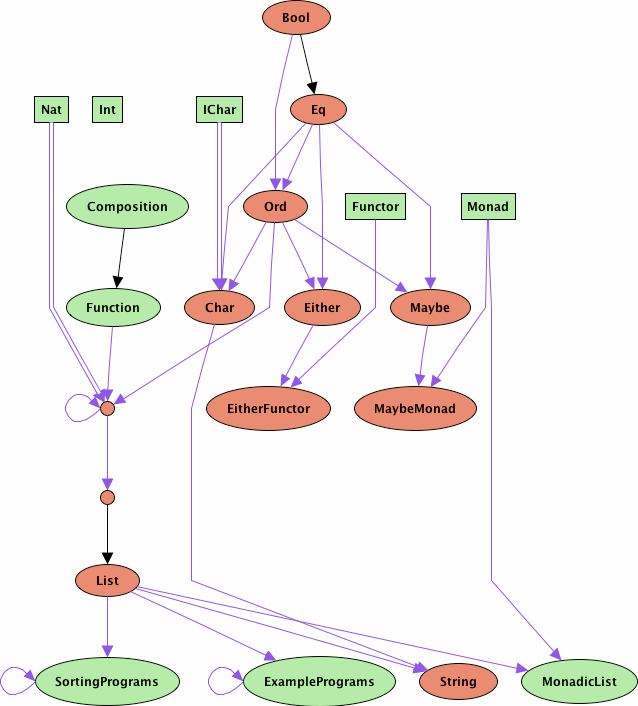
\includegraphics[scale=0.9]{figuras/ProofStart.png}
    \caption{Estado inicial das provas da biblioteca na ferramenta Hets}
    \label{fig:ProofStart}
\end{figure}

Na figura, os nós elípticos representam uma especificação do arquivo que foi analisado.
Os círculos indicam subespecificações, ou seja, trechos de especificações que foram separados pela declaração \Verb.then..
Os retângulos indicam especificações importadas de outras bibliotecas.
No caso deste trabalho, todas foram importadas da biblioteca da linguagem \CASL.
Os nós vermelhos (cinza escuro) indicam especificações que possuem um ou mais teoremas a serem provados.
Os nós verdes (cinza claro) não possuem teoremas ou todos os seus teoremas já estão provados.

A partir do grafo pode-se iniciar o provador de teoremas \Isabelle para verificar os teoremas existentes nos nós. Uma prova típica se inicia pelo método automático de prova sobre a estrutura da especificação. Este método analisa as teorias presentes e as diretivas (\Verb.%mono., \Verb.%implies., etc.), construindo as dependências entre as especificações e revelando os nós ocultos das subespecificações que contêm teoremas a serem provados.

O próximo passo é utilizar o provador \Isabelle para verificar os teoremas existentes nos nós vermelhos. Para tanto, basta escolher um nó e, com o botão direito, escolher a opção \textit{Prove}. A janela seguinte permite escolher um entre vários provadores de teoremas. Para a linguagem \HasCASL, o provador \Isabelle precisa ser usado. Esta opção irá efetuar a tradução da especificação para uma teoria correspondente em \HOL, exibindo a mesma em uma outra janela do editor \textit{emacs}, permitindo com que a prova dos teoremas seja escrita.

Após processar todo o arquivo de provas, pode-se fechar o editor de texto e o estado desta prova será atualizado no grafo. Se a prova foi finalizada com sucesso, o nó correspondente terá sua cor alterada para verde. Caso contrário, sua cor permanecerá vermelha. Quando todos os nós circulares correspondentes a subespecificações de um nó elíptico tiverem a cor alterada para verde, eles novamente se tornarão ocultos, e apenas o nó elíptico correspondente à especificação completa será exibido.

Algumas provas de teoremas da especificação da biblioteca ainda permanecem em aberto, como ilustram os nós vermelhos da \citeFig{fig:ProofEnd}. Os nós amarelos indicam a necessidade de aplicar verificações de consistência em relação ao monomorfismo (indicado na especificação pela diretiva \Verb_%mono_). A maior parte das provas em aberto estão relacionadas à falta de suporte de construtores de classes na linguagem \HOL. Métodos alternativos de tradução para \Isabelle/\HOL estão em investigação pelo grupo responsável pela ferramenta \Hets.

\begin{figure}[hp]
    \centering
        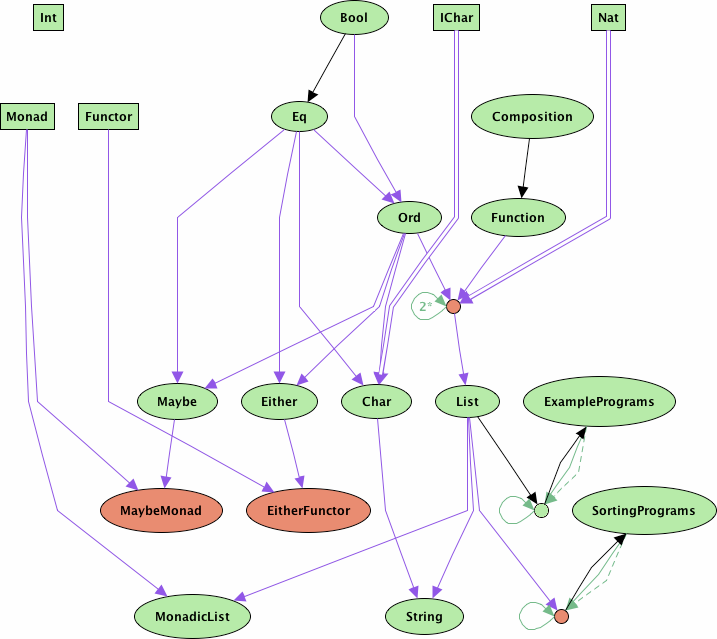
\includegraphics[scale=0.9]{figuras/ProofEnd.png}
    \caption{Estado final das provas da biblioteca na ferramenta Hets}
    \label{fig:ProofEnd}
\end{figure}

\section{Usando o provador de teoremas Isabelle}
A tarefa de verificar os teoremas gerados pela especificação, embora não fosse o foco do trabalho, tornou-se a parte mais complexa. Embora ainda permaneçam teoremas em aberto, a maioria pode ser verificado. A seguir, explica-se como se deu o processo de construção das provas.

A maior parte das provas foi iniciada pelo comando \Verb.apply(auto). porque desejava-se que \Isabelle agisse de forma automática, sempre que possível. Abaixo, ilustra-se a prova de um teorema da especificação \Verb.Bool.:

\begin{Verbatim}
theorem NotFalse1 : "ALL x.
 Not' x = True' = (x = False')"
apply(auto)
apply(case_tac x)
apply(auto)
done
\end{Verbatim}

A seguir, os comandos da prova são explicados:
\begin{itemize}
\item \textit{apply (auto)}:

Este comando simplifica a proposição atual de forma automática, indo o mais longe que conseguir nas reduções.
Neste teorema, o comando apenas conseguiu eliminar o quantificador universal, produzindo o resultado a seguir:

\begin{Verbatim}
goal (1 subgoal):
 1. !!x. Not' x = True' ==> x = False'
\end{Verbatim}

\item \textit{apply (case\_tac x)}:

O método \textit{case\_tac} atribui uma valoração possível para a variável \Verb.x., substituindo-a por cada um dos construtores do tipo a que a variável pertence.
Aqui, como a variável \Verb.x. é do tipo \Verb.Bool., \Verb.x. foi instanciado para os construtores \Verb.True. e \Verb.False.:

\begin{Verbatim}
goal (2 subgoals):
 1. !!x. [| Not' x = True'; x = False' |] ==> x = False'
 2. !!x. [| Not' x = True'; x = True' |] ==> x = False'
\end{Verbatim}

\item \textit{apply (auto)}:

Desta vez, o comando automático foi capaz de terminar a prova automaticamente.

\begin{Verbatim}
goal:
No subgoals!
\end{Verbatim}

\end{itemize}

Um exemplo de prova para um teorema da especificação \Verb.Eq. é mostrado a seguir.
Nesta prova, foi introduzido o comando \Verb.simp add:., que espera uma lista de axiomas ou teoremas previamente provados como parâmetros para serem utilizados em uma tentativa automática de simplificar a proposição corrente.
Este comando faz uso, além dos teoremas passados como parâmetro, dos demais axiomas no escopo da teoria atual.
Se a proposição não pode ser reduzida, o comando produz um erro; caso contrário, uma nova proposição é gerada, caso a prova não tenha sido concluída automaticamente.

\begin{Verbatim}
theorem DiffTDef :
"ALL x. ALL y. x /= y = True' 
= (Not' (x ==' y) = True')"
apply(auto)
apply(simp add: DiffDef)
apply(case_tac "x ==' y")
apply(auto)
apply(simp add: DiffDef)
done
\end{Verbatim}

Os teoremas usados na prova anterior também foram utilizados em várias provas da especificação \Verb.Ord..
A prova do teorema \Verb.%(LeTAssimetry)%. destaca-se das demais por introduzir a necessidade de criar lemas auxiliares.
Em alguns casos, um axioma ou teorema precisa ser reescrito de forma que o \Isabelle consiga utilizá-lo em suas provas automáticas.
Para tanto, cria-se um lema, que apesar do nome, funciona da mesma forma que um teorema.
No caso do teorema \Verb.%(LeTAssimetry)%., utilizou-se o comando \Verb.rule ccontr. para iniciar uma prova por contradição.
Após algumas simplificações, o provador \Isabelle não foi capaz de utilizar o axioma \Verb.%(LeIrreflexivity)%. para simplificar o objetivo e produziu:

\begin{Verbatim}
goal (1 subgoal):
 1. !!x y. [| x <' y = True'; y <' x = True' |] ==> False
\end{Verbatim}

Foi necessário criar o lema auxiliar \Verb.LeIrreflContra., provado automaticamente pelo provador \Isabelle.
O teorema foi interpretado internamente da seguinte forma:

\begin{Verbatim}
?x <' ?x = True' ==> False
\end{Verbatim}

Pode-se, então, induzir a ferramenta \Isabelle a usar o lema anterior forçando a atribuição do valor \Verb.x. para a variável \Verb.?x. através do comando \Verb.rule_tac x="x" in LeIrreflContra..
A mesma tática foi utilizada para forçar o uso do axioma \Verb.%(LeTTransitive)%..
A prova foi finalizada com o comando \Verb.by auto..

\begin{Verbatim}
lemma LeIrreflContra :
  " x <' x = True' ==> False"
by auto

theorem LeTAsymmetry :
"ALL x. ALL y. x <' y = True'
  --> y <' x = False'"
apply(auto)
apply(rule ccontr)
apply(simp add: notNot2 NotTrue1)
apply(rule_tac x="x" in LeIrreflContra)
apply(rule_tac y="y" in LeTTransitive)
by auto
\end{Verbatim}

Alguns usos do comando \Verb.apply(auto). podem entrar em laços infinitos.
Um exemplo ocorreu quando os teoremas das especificações \Verb.Maybe. e \Verb.Either. foram provados.
Para evitar o laço infinito, a regra de eliminação do quantificador universal foi aplicada diretamente, usando o comando \Verb.apply(rule allI)..
O comando \Verb.rule. aplica o teorema ou axioma especificado diretamente, sem usar outras regras na redução.
Para remover mais de um quantificador, pode-se incluir o sinal \Verb.+. após a regra, indicando que a mesma deve ser utilizada repetidamente, até que não seja possível nenhuma outra simplificação.

Após remover os quantificadores, o comando \Verb.simp only:. foi aplicado.
Este comando, ao contrário do comando \Verb.simp add:., utiliza apenas as regras passadas como parâmetros para tentar simplificar o objetivo atual.
Na maior parte das vezes, os dois comandos podem ser usados sem distinção.
Algumas vezes, no entanto, o comando \Verb.simp add:. pode entrar em laços infinitos; nestes casos, o comando \Verb.simp only:. deve ser usado para que a simplificação seja possível.
Abaixo, mostra-se um teorema e sua respectiva prova para exemplificar o procedimento descrito.

\begin{Verbatim}
theorem IMO03 : "ALL x. Nothing >=' Just(x) = False'"
apply(rule allI)
apply(simp only: GeqDef)
apply(simp only: GeDef OrDef)
apply(case_tac "Just(x) <' Nothing")
apply(auto)
done
\end{Verbatim}

A especificação \Verb.ListNoNumbers. possui apenas o teorema \Verb.FoldlDecomp. em aberto.
Já a especificação \Verb.ListWithNumbers., que possui quatro teoremas, tem todos os seus teoremas em aberto.
No primeiro caso, quase todos os teoremas necessitaram de comandos de indução para serem provados.
\Isabelle executa indução sobre uma variável através do comando \Verb.induct_tac..
Este comando espera como parâmetro uma variável ou uma expressão sobre a qual deve executar o processo de indução.
A seguir, é apresentado um exemplo envolvendo indução oriundo da especificação \Verb.ListNoNumbers..

\begin{Verbatim}
theorem FilterProm :
"ALL f. ALL p. ALL xs.
 X_filter p (X_map f xs) = 
   X_map f (X_filter 
     (X__o__X (p, f)) xs)"
apply(auto)
apply(induct_tac xs)
apply(auto)
apply(case_tac "p(f a)")
apply(auto)
apply(simp add: MapCons)
apply(simp add: FilterConsT)
apply(simp add: MapCons)
apply(simp add: FilterConsT)
done
\end{Verbatim}

As especificações \Verb.Char. e \Verb.String. usam combinações de comandos apresentados nos exemplos acima e, dessa forma, não são exemplificadas aqui.

As provas da especificação do exemplo \Verb.ExamplePrograms. embora longas, usaram apenas três comandos, basicamente: \Verb.simp only:., \Verb.case_tac., e \Verb.simp add:..
Como o comando \Verb.simp add:. consegue, geralmente, simplificações maiores, optou-se por tentar usá-lo sempre que possível.
Nos casos em que o comando entrou em laços infinitos, ele foi trocado pelo comando \Verb.simp only:..
Um teorema nesta especificação ainda permanece em aberto.
A seguir, a prova do teorema \Verb.Program02. é mostrada como exemplo.

\begin{Verbatim}
theorem Program02 :
"quickSort(X_Cons True' (X_Cons False' Nil')) =
 X_Cons False' (X_Cons True' Nil')"
apply(simp only: QuickSortCons)
apply(case_tac "(%y. y <' True') False'")
apply(simp only: FilterNil FilterConsT FilterConsF)
apply(simp only: QuickSortNil)
apply(simp only: XPlusXPlusNil)
apply(simp only: XPlusXPlusCons)
apply(simp only: XPlusXPlusNil)
apply(case_tac "(%y. y >=' True') False'")
apply(simp only: FilterNil FilterConsT FilterConsF)
apply(simp only: QuickSortNil)
apply(simp add: LeFGeTEqTRel)
apply(simp only: FilterNil FilterConsT FilterConsF)
apply(simp only: QuickSortCons)
apply(simp only: FilterNil FilterConsT FilterConsF)
apply(simp only: QuickSortNil)
apply(simp only: XPlusXPlusNil)
apply(simp only: XPlusXPlusCons)
apply(simp only: XPlusXPlusNil)
apply(simp only: IBO5)
apply(simp only: FilterNil FilterConsT FilterConsF)
apply(simp only: QuickSortCons)
apply(simp only: FilterNil FilterConsT FilterConsF)
apply(simp only: QuickSortNil)
apply(simp only: XPlusXPlusNil)
apply(simp only: XPlusXPlusCons)
apply(simp only: XPlusXPlusNil)
apply(case_tac "(%y. y >=' True') False'")
apply(simp only: FilterNil FilterConsT FilterConsF)
apply(simp only: QuickSortNil)
apply(simp only: XPlusXPlusCons)
apply(simp only: XPlusXPlusNil)
apply(simp only: FilterNil FilterConsT FilterConsF)
apply(simp only: QuickSortCons)
apply(simp only: FilterNil FilterConsT FilterConsF)
apply(simp only: QuickSortNil)
apply(simp only: XPlusXPlusNil)
apply(simp only: XPlusXPlusCons)
apply(simp only: XPlusXPlusNil)
apply(simp add: LeFGeTEqTRel)
done
\end{Verbatim}

Todos os teoremas da especificação \Verb.SortingPrograms. ainda não tiveram suas provas finalizadas.
Embora, para todos eles, várias proposições intermediárias tenham sido provadas, o caso geral ainda permanece em aberto.
Para mostrar o progresso feito nas provas, um exemplo com alguns comentários é apresentado a seguir.
O comando \Verb.prefer. é utilizado para escolher qual proposição se quer provar ao se utilizar o provador \Isabelle no modo interativo.
O comando \Verb.oops. indica ao provador para desistir da prova e seguir em frente no arquivo de provas.

\begin{Verbatim}
theorem Theorem07 : "ALL xs. isOrdered(insertionSort(xs))"
apply(auto)
apply(case_tac xs)
(* Proof for xs=Nil *)
prefer 2
apply(simp only: InsertionSort)
apply(simp add: GenSortF)
(* Proof for general case *)
apply(simp only: InsertionSort)
apply(case_tac List)
apply(auto)
apply(case_tac "X_splitInsertionSort (X_Cons a (X_Cons aa Lista))")
(* Proof for xs= Cons a Nil *)
prefer 2
apply(simp add: GenSortF)
(* Proof for xs=Cons a as*)
apply(case_tac Lista)
apply(auto)
prefer 2
(* Proof for xs = Cons a (Cons b Nil)*)
oops
\end{Verbatim}

\chapter{Uma Extensão para Inclusão de Suporte à Avaliação Preguiçosa}
\label{chap:laziness}

Na linguagem \HasCASL, assim como no $\lambda$-cálculo parcial, a avaliação de tipos é estrita, ao contrário da linguagem \Haskell, que implementa a avaliação preguiçosa de tipos, permitindo que funções com argumentos indefinidos tenham resultados definidos sempre que os argumentos indefinidos não forem necessários no corpo da função.

O suporte à avaliação preguiçosa pode ser incluído em especificações escritas em \HasCASL em dois níveis.
Em uma abordagem mais simples, pode-se apenas utilizar a avaliação preguiçosa sem o uso de tipos que permitam a execução de especificações e a simulação do comportamento de funções da linguagem \Haskell.
A abordagem mais complexa, por sua vez, exige a alteração do domínio semântico das funções em \HasCASL para um subconjunto de tipos onde a noção de especificação executável pode ser definida, permitindo recursão e não-terminação de programas.
A seguir, discutimos as duas abordagens, detalhando a aplicação da primeira no projeto.

\section{Tipos com avaliação preguiçosa}
Em uma linguagem com avaliação estrita, o suporte à avaliação preguiçosa pode ser emulado substituindo-se um tipo com avaliação estrita \Verb.T. nas declarações de funções e variáveis por um tipo de função \Verb.Unit -> ?T., que na linguagem \HasCASL pode ser abreviado pelo tipo \Verb.?T..
Quando a alteração ocorrer em uma função parcial envolvendo tipos com avaliação estrita, a mesma será alterada para uma função total envolvendo tipos com avaliação preguiçosa, isto é, uma função parcial \Verb. T ->? S., ao incorporar tipos com avaliação preguiçosa, deve ser alterada para a função total \Verb.?T -> ?S..~\cite{SchroderMossakowski08}
Vale notar que a função total \Verb.T1 -> T2 -> ... -> ?S., com imagem no tipo com avaliação preguiçosa \Verb.?S., equivale à função parcial \Verb.T1 -> T2 -> ... ->? S, com imagem no tipo com avaliação estrita \Verb.S., sendo indiferente o posicionamento do sinal de interrogação, neste caso.

Ao declararem-se novos tipos, os construtores de tipos que dependem de variáveis de tipo com avaliação estática devem alterar estas variáveis para suportar avaliação preguiçosa e, também, devem ser alterados para serem construtores parciais, incluindo-se o sinal \Verb.?. depois dos parâmetros do construtor.
Por exemplo, o tipo \Verb.List., declarado como \Verb.free type List a ::= Nil | Cons a (List a). com suporte a avaliação estrita, deve ser alterado, a fim de suportar a avaliação preguiçosa, para:

\begin{minipage}[t]{0.9\linewidth}
\begin{Verbatim}
free type List a ::= Nil | Cons (?a) (?List a)?
\end{Verbatim}
\end{minipage}

Embora a avaliação do tipo tupla seja estrita em \HasCASL, tuplas formadas por tipos com avaliação preguiçosa puderam ser utilizadas como parâmetros de funções na biblioteca deste trabalho.
No entanto, esta abordagem gera problemas na composição de tipos através de tuplas, como como no tipo para listas de tuplas (\Verb.?List (?a,?b).).
Uma solução para este problema seria a criação de um novo tipo com avaliação preguiçosa:

\begin{minipage}[t]{0.9\linewidth}
\begin{Verbatim}
free type Pair a b ::= Pair (?a) (?b)?
\end{Verbatim}
\end{minipage}

e o seu uso ao invés das tuplas, tal como em \Verb.?List (?Pair a b)..

O tipo de dado \Verb.Bool. foi alterado de forma especial, a fim de mapeá-lo para o tipo de valores booleanos presente na linguagem \HasCASL.
Definido anteriormente como \Verb.free type Bool ::= True | False., este tipo foi redefinido como \Verb.type Bool := ?Unit..
Por esta associação, a constante \Verb.true. é associada ao elemento do conjunto unitário \Verb.Unit. e qualquer outro valor ou a ausência de um valor são associados à constante \Verb.false..
Este mesmo comportamento existe para os operadores lógicos de \HasCASL, também definidos sobre o tipo \Verb.?Unit..
Com este mapeamento, as aplicações de funções com tipo de retorno \Verb.Bool. são interpretadas como predicados, tornando possível a remoção da comparação com os construtores \Verb.True. e \Verb.False. nos axiomas e teoremas, uma vez que um axioma passa a determinar um valor verdadeiro e valores que não estão definidos por axiomas passam a ser considerados falsos.
O mapeamento também simplifica as provas realizadas com a ferramenta \Hets, uma vez que o tipo de dado \Verb.?Unit. é mapeado para o tipo de dado \Verb.bool. de \HOL.

\pagebreak

O tipo de dados \Verb.Bool. após o refinamento pode ser visto a seguir:

\begin{Verbatim}
spec Bool = %mono
type Bool := ?Unit 
fun Not__ : ?Bool -> ?Bool
fun __&&__ : ?Bool * ?Bool -> ?Bool
fun __||__ : ?Bool * ?Bool -> ?Bool
fun otherwiseH: ?Bool      
vars x,y: ?Bool
. Not(false)                        %(NotFalse)%
. not Not(true)                     %(NotTrue)%
. not (false && x)                  %(AndFalse)%
. true && x = x                     %(AndTrue)%
. x && y = y && x                   %(AndSym)%
. x || y = Not(Not(x) && Not(y))    %(OrDef)%
. otherwiseH                        %(OtherwiseDef)%
. (Not x) = not x           %(NotFalse1)% %implied
. not (Not x) = x           %(NotTrue1)% %implied
. (not x) = Not x           %(notNot1)% %implied
. (not not x) = not Not x   %(notNot2)% %implied
end
\end{Verbatim}

O suporte à avaliação preguiçosa ainda está em fase de desenvolvimento.
A aplicação deste tipo de avaliação no tipo \Verb.List List a., por exemplo, pode gerar o tipo \Verb.?List List a. ou o tipo \Verb.?List(?List(?a))..
Nenhum destes tipos gera erro sintático na ferramenta \Hets, embora o segundo tipo seja o tipo correto.
A tradução do segundo tipo para a linguagem \HOL, neste momento, ainda não reflete o seu poder de expressão e não permite, também, o desenvolvimento de provas envolvendo este tipo.
Dessa forma, apenas as especificações \Verb.Bool., \Verb.Eq., \Verb.Ord., \Verb.Maybe. e \Verb.Either. tiveram todos os seus teoremas provados.
As demais especificações ou possuem a maior parte dos teoremas em aberto ou não puderam ter as provas iniciadas pela falta de suporte no processo de tradução.

A aplicação destas alterações na biblioteca pode ser conferida no \citeAppendix{appendix:lazySpec}, e as provas para esta versão da biblioteca encontram-se no \citeAppendix{appendix:lazyProofs}.

\section{Recursão e não-terminação de programas}
A aplicação de tipos com avaliação preguiçosa definidos da forma descrita anteriormente não simula o comportamento da linguagem de programação \Haskell, impedindo o uso de recursão e de estruturas de dados infinitas.
Estas estruturas e a possibilidade de não-terminação de programas exigem o uso de um novo domínio semântico, tanto nas especificações escritas em \HasCASL quanto nas provas escritas para a ferramenta \Isabelle.
Este domínio representa um subconjunto de tipos onde a noção de especificação executável é permitida, ou seja, onde as especificações podem ser interpretadas como programas escritos em linguagens de programação funcional.

O domínio de especificações executáveis em \HasCASL pode ser usado através das classes \Verb.Cpo. e \Verb.Cppo., definidas na especificação \Verb.Recursion. da biblioteca \Verb.HasCASL/Metatheory/Recursion. e transcritos a seguir:

\begin{Verbatim}
spec Recursion = Ord with Ord |-> InfOrd, __<=__ |-> __<<=__ and Nat then
class  Cpo < InfOrd {
var    a: Cpo
fun    __<<=__ : Pred (a * a)
op     undefined: ?a
. not def (undefined: ?a)
type   Chain a = {s: Nat ->? a . forall n: Nat . def s n => s n <<= s (n + 1)}
fun    sup: Chain a ->? a
var    x: ?a; c: Chain a
. sup c <<=[?a] x <=> forall n: Nat . c n <<=[?a] x
}

class Cppo < Cpo {
var    a : Cppo
fun    bottom : a
. bottom <<= x
}

class FlatCpo < Cpo {
vars   a : FlatCpo; x, y: a
. x <<= y => x = y
}

vars a, b: Cpo; c: Cppo; x, y: a; z, w: b
type instance __*__ : +Cpo -> +Cpo -> Cpo
type instance __*__ : +Cppo -> +Cppo -> Cppo

type instance Unit : Cppo
type instance Unit : FlatCpo

type a -->? b = { f : a ->? b . forall c: Chain a .
                 sup ((\ n: Nat . f (c n)) as Chain b) = f (sup c) }

type a --> b = { f : a -->? b . f in a -> b }

type instance __-->?__ : -Cpo -> +Cpo -> Cppo
var  f, g: a -->? b
. f <<= g <=> forall x: a . def (f x) => f x <<= g x

type instance __-->__ : -Cpo -> +Cpo -> Cpo
var  f, g: a --> b
. f <<= g <=> forall x: a . f x <<= g x

type instance __-->__ : -Cpo -> +Cppo -> Cppo
. bottom[a --> c] = \ x: a . bottom[c]

then %def

var c: Cppo
fun Y : (c --> c) --> c
var f : c --> c; x: c; P : Pred c
. f(Y f) = Y f
. f x = x => Y f <<= x
. P bottom /\ (forall x : c . P x => P (f x)) => P (Y f) %implied
\end{Verbatim}

Os tipos de dados utilizados em especificações que suportem recursão devem ser instâncias das classes \Verb.Cpo. ou \Verb.Cppo. e, quando polimórficos, devem estar definidos sobre variáveis de tipos que sejam instâncias destas classes.
Um tipo de dado nesta semântica pode ser definido com o uso da palavra-chave \Verb.free domain., como a seguir:

\begin{Verbatim}
var a : Cpo
free domain List a ::= Nil | Cons a (List a)
\end{Verbatim}

O tipo de dado definido acima representa uma lista finita de elementos cujo tipo é instância da classe \Verb.Cpo..
Esta lista pode ser utilizada em funções recursivas, embora ainda não capture as noções de listas com avaliação preguiçosa e nem de listas infinitas.

Para representar listas com avaliação preguiçosa e listas infinitas, deve-se definir o tipo de dado da seguinte forma:

\begin{Verbatim}
var a : Cpo
free domain LList a ::= Nil | Cons a ?(LList a)
\end{Verbatim}

As listas infinitas podem ser criadas através de uma cadeia de listas finitas com avaliação preguiçosa.

\HasCASL permite, dentro deste domínio, que funções recursivas sejam definidas como equações recursivas no estilo de linguagens de programação funcional, tal como \Haskell, bastando defini-las após a palavra-chave \Verb.program..
A tradução destas equações para os termos que façam uso do operador de ponto fixo definido na especificação \Verb.Recursion. é implícita.

Pode-se, como no domínio padrão de \HasCASL, definir funções com avaliação estrita ou preguiçosa de tipos de dados.
A definição de funções com avaliação preguiçosa dentro deste domínio semântico produz especificações com comportamento equivalente ao comportamento encontrado na linguagem \Haskell.

Para escrever provas na ferramenta \Isabelle dentro deste domínio é necessário alterar a lógica utilizada de \HOL para \HOLCF.
O suporte à tradução para a teoria \HOLCF pela ferramenta \Hets ainda está em desenvolvimento e a complexidade do uso desta lógica é muito maior do que a do uso da lógica \HOL.

O uso desta abordagem para avaliação preguiçosa não foi implementado porque exigiria mais tempo do que o disponível para a confecção deste trabalho.
Notadamente, a necessidade de aprender mais uma lógica associada ao provador \Isabelle demandaria um tempo consideravelmente grande.

\bibliography{Dissertacao,cofi}

\newpage
%Apêndices
\appendix

\renewcommand{\appendixpagename}{Apêndices}
\appendixpage

\fvset{fontsize=\relsize{-1}}
\chapter{Listagem das Especificações com Avaliação Estrita Desenvolvidas em HasCASL}
\label{appendix:strictSpec}
Este apêndice contém o código das especificações com avaliação estrita desenvolvidas neste trabalho com o uso da linguagem \HasCASL.
O arquivo-fonte pode ser reconstruído compiando-se todas as especificações aqui descritas, na ordem apresentada, em um arquivo \textit{Prelude.hs}.

\section{Cabeçalhos da Biblioteca \textit{Prelude}}
\label{appendix:strictSpec:header}
\begin{Verbatim}
library Prelude
version 0.1
%authors: Glauber M. Cabral <glauber.sp@gmail.com>
%date: 19 Fev 2008

logic HasCASL 

from Basic/Numbers get Nat, Int, Rat
from HasCASL/Metatheory/Monad get Functor, Monad
from Basic/CharactersAndStrings get Char |-> IChar
\end{Verbatim}

\section{Especificação \textit{Bool}}
\label{appendix:strictSpec:bool}
\begin{Verbatim}
spec Bool = %mono
free type Bool ::= True | False 
fun Not__ : Bool -> Bool
fun __&&__ : Bool * Bool -> Bool
fun __||__ : Bool * Bool -> Bool
fun otherwiseH: Bool      
vars x,y: Bool
. Not(False) = True %(NotFalse)%
. Not(True) = False                 %(NotTrue)%
. False && x = False                %(AndFalse)%
. True && x = x                     %(AndTrue)%
. x && y = y && x                   %(AndSym)%
. x || y = Not(Not(x) && Not(y))    %(OrDef)%
. otherwiseH = True                 %(OtherwiseDef)%
%% 
. Not x = True <=> x = False        %(NotFalse1)% %implied
. Not x = False <=> x = True        %(NotTrue1)% %implied
. not (x = True) <=> Not x = True   %(notNot1)% %implied
. not (x = False) <=> Not x = False %(notNot2)% %implied
end
\end{Verbatim}

\section{Especificação \textit{Eq}}
\label{appendix:strictSpec:eq}
\begin{Verbatim}
spec Eq = Bool then
class Eq {
var a: Eq
fun __==__ : a * a -> Bool
fun __/=__ : a * a -> Bool
vars x,y,z: a
. x = y => (x == y) = True                                %(EqualTDef)%
. x == y = y == x                                         %(EqualSymDef)%
. (x == x) = True                                         %(EqualReflex)%
. (x == y) = True /\ (y == z) = True => (x == z) = True   %(EqualTransT)%
. (x /= y) = Not (x == y)                                 %(DiffDef)%
. (x /= y) = (y /= x)                                     %(DiffSymDef)% %implied
. (x /= y) = True <=> Not (x == y) = True                 %(DiffTDef)% %implied
. (x /= y) = False <=> (x == y) = True                    %(DiffFDef)% %implied
. (x == y) = False => not (x = y)            %(TE1)% %implied
         %% == and Not need to be related!
. Not (x == y) = True <=> (x == y) = False   %(TE2)% %implied
. Not (x == y) = False <=> (x == y) = True   %(TE3)% %implied
. not ((x == y) = True) <=> (x == y) = False %(TE4)% %implied
}
type instance Bool: Eq
. (True == True) = True                %(IBE1)% %implied
. (False == False) = True              %(IBE2)% %implied
. (False == True) = False              %(IBE3)%
. (True == False) = False              %(IBE4)% %implied
. (True /= False) = True               %(IBE5)% %implied
. (False /= True) = True               %(IBE6)% %implied
. Not (True == False) = True           %(IBE7)% %implied
. Not (Not (True == False)) = False    %(IBE8)% %implied
type instance Unit: Eq
. (() == ()) = True  %(IUE1)% %implied
. (() /= ()) = False %(IUE2)% %implied
end
\end{Verbatim}

\section{Especificação \textit{Ord}}
\label{appendix:strictSpec:ord}
\begin{Verbatim}
spec Ord = Eq and Bool then
free type Ordering ::= LT | EQ | GT
type instance Ordering: Eq
. (LT == LT) = True   %(IOE01)% %implied
. (EQ == EQ) = True   %(IOE02)% %implied
. (GT == GT) = True   %(IOE03)% %implied
. (LT == EQ) = False  %(IOE04)%
. (LT == GT) = False  %(IOE05)%
. (EQ == GT) = False  %(IOE06)%
. (LT /= EQ) = True   %(IOE07)% %implied
. (LT /= GT) = True   %(IOE08)% %implied
. (EQ /= GT) = True   %(IOE09)% %implied
class Ord < Eq
{
 var a: Ord
 fun compare: a -> a -> Ordering
 fun __<__ : a * a -> Bool
 fun __>__ : a * a -> Bool
 fun __<=__ : a * a -> Bool
 fun __>=__ : a * a -> Bool
 fun min: a -> a -> a
 fun max: a -> a -> a
 var    x, y, z, w: a
%% Definitions for relational operations.
%% Axioms for <
 . (x == y) = True => (x < y) = False                      %(LeIrreflexivity)%
 . (x < y) = True => y < x = False                         %(LeTAsymmetry)% %implied
 . (x < y) = True /\ (y < z) = True => (x < z) = True      %(LeTTransitive)%
 . (x < y) = True \/ (y < x) = True \/ (x == y) = True     %(LeTTotal)%
%% Axioms for >
 . (x > y) = (y < x)                                    %(GeDef)%
 . (x == y) = True => (x > y) = False                   %(GeIrreflexivity)% %implied
 . (x > y) = True => (y > x) = False                    %(GeTAsymmetry)% %implied
 . ((x > y)  && (y > z)) = True => (x > z) = True       %(GeTTransitive)% %implied
 . (((x > y) || (y > x)) || (x == y)) = True            %(GeTTotal)% %implied 
%% Axioms for <=
 . (x <= y) = (x < y) || (x == y)                         %(LeqDef)%
 . (x <= x) = True                                        %(LeqReflexivity)% %implied
 . ((x <= y) && (y <= z)) = True => (x <= z) = True       %(LeqTTransitive)% %implied
 . (x <= y) && (y <= x) = (x == y)                        %(LeqTTotal)% %implied
%% Axioms for >=
 . (x >= y) = ((x > y) || (x == y))                 %(GeqDef)%
 . (x >= x) = True                                  %(GeqReflexivity)% %implied 
 . ((x >= y) && (y >= z)) = True => (x >= z) = True %(GeqTTransitive)% %implied
 . (x >= y) && (y >= x) = (x == y)                  %(GeqTTotal)% %implied
%% Relates == and ordering
 . (x == y) = True <=> (x < y) = False /\ (x > y) = False  %(EqTSOrdRel)%
 . (x == y) = False <=> (x < y) = True \/ (x > y) = True   %(EqFSOrdRel)%
 . (x == y) = True <=> (x <= y) = True /\ (x >= y) = True  %(EqTOrdRel)%
 . (x == y) = False <=> (x <= y) = True \/ (x >= y) = True %(EqFOrdRel)%
 . (x == y) = True /\ (y < z) = True => (x < z) = True     %(EqTOrdTSubstE)%
 . (x == y) = True /\ (y < z) = False => (x < z) = False   %(EqTOrdFSubstE)%
 . (x == y) = True /\ (z < y) = True => (z < x) = True     %(EqTOrdTSubstD)%
 . (x == y) = True /\ (z < y) = False => (z < x) = False   %(EqTOrdFSubstD)%
 . (x < y) = True <=> (x > y) = False /\ (x == y) = False %(LeTGeFEqFRel)%
 . (x < y) = False <=> (x > y) = True \/ (x == y) = True  %(LeFGeTEqTRel)%
%% Relates all the ordering operators with True as result.
 . (x < y) = True <=> (y > x) = True     %(LeTGeTRel)% %implied
 . (x < y) = False <=> (y > x) = False   %(LeFGeFRel)% %implied
 . (x <= y) = True <=> (y >= x) = True   %(LeqTGetTRel)% %implied
 . (x <= y) = False <=> (y >= x) = False %(LeqFGetFRel)% %implied
 . (x > y) = True <=> (y < x) = True     %(GeTLeTRel)% %implied
 . (x > y) = False <=> (y < x) = False   %(GeFLeFRel)% %implied
 . (x >= y) = True <=> (y <= x) = True   %(GeqTLeqTRel)% %implied
 . (x >= y) = False <=> (y <= x) = False %(GeqFLeqFRel)% %implied
%%
 . (x <= y) = True <=> (x > y) = False                    %(LeqTGeFRel)% %implied
 . (x <= y) = False <=> (x > y) = True                    %(LeqFGeTRel)% %implied
 . (x > y) = True <=> (x < y) = False /\ (x == y) = False %(GeTLeFEqFRel)% %implied
 . (x > y) = False <=> (x < y) = True \/ (x == y) = True  %(GeFLeTEqTRel)% %implied
 . (x >= y) = True <=> (x < y) = False                    %(GeqTLeFRel)% %implied
 . (x >= y) = False <=> (x < y) = True                    %(GeqFLeTRel)% %implied
%%
 . (x <= y) = True <=> (x < y) = True \/ (x == y) = True    %(LeqTLeTEqTRel)% %implied
 . (x <= y) = False <=> (x < y) = False /\ (x == y) = False %(LeqFLeFEqFRel)% %implied
 . (x >= y) = True <=> (x > y) = True \/ (x == y) = True    %(GeqTGeTEqTRel)% %implied
 . (x >= y) = False <=> (x > y) = False /\ (x == y) = False %(GeqFGeFEqFRel)% %implied
%%
%% Implied True - False relations.
 . (x < y) = True <=> (x >= y) = False  %(LeTGeqFRel)% %implied
 . (x > y) = True <=> (x <= y) = False  %(GeTLeqFRel)% %implied
 . (x < y) = (x <= y) && (x /= y)       %(LeLeqDiff)% %implied
%% Definitions with compare 
%% Definitions to compare, max and min using relational operations.
 . (compare x y == LT) = (x < y)                       %(CmpLTDef)%
 . (compare x y == EQ) = (x == y)                      %(CmpEQDef)%
 . (compare x y == GT) = (x > y)                       %(CmpGTDef)%
%% Define min, max
 . (max x y == y) = (x <= y)                          %(MaxYDef)%
 . (max x y == x) = (y <= x)                          %(MaxXDef)%
 . (min x y == x) = (x <= y)                          %(MinXDef)%
 . (min x y == y) = (y <= x)                          %(MinYDef)%
 . (max x y == y) = (max y x == y)                    %(MaxSym)% %implied
 . (min x y == y) = (min y x == y)                    %(MinSym)% %implied
}
%% Theorems
 . (x == y) = True \/ (x < y) = True <=> (x <= y) = True                  %(TO1)% %implied
 . (x == y) = True  => (x < y) = False                                    %(TO2)% %implied
 . Not (Not (x < y)) = True \/ Not (x < y) = True                         %(TO3)% %implied
 . (x < y) = True => Not (x == y) = True                                  %(TO4)% %implied
 . (x < y) = True /\ (y < z) = True /\ (z < w) = True => (x < w) = True   %(TO5)% %implied
 . (z < x) = True => Not (x < z) = True                                   %(TO6)% %implied
 . (x < y) = True <=> (y > x) = True                                      %(TO7)% %implied
 type instance Ordering: Ord
 . (LT < EQ) = True                     %(IOO13)%
 . (EQ < GT) = True                     %(IOO14)%
 . (LT < GT) = True                     %(IOO15)%
 . (LT <= EQ) = True                    %(IOO16)% %implied
 . (EQ <= GT) = True                    %(IOO17)% %implied
 . (LT <= GT) = True                    %(IOO18)% %implied
 . (EQ >= LT) = True                    %(IOO19)% %implied
 . (GT >= EQ) = True                    %(IOO20)% %implied
 . (GT >= LT) = True                    %(IOO21)% %implied
 . (EQ > LT) = True                     %(IOO22)% %implied
 . (GT > EQ) = True                     %(IOO23)% %implied
 . (GT > LT) = True                     %(IOO24)% %implied
 . (max LT EQ == EQ) = True             %(IOO25)% %implied
 . (max EQ GT == GT) = True             %(IOO26)% %implied
 . (max LT GT == GT) = True             %(IOO27)% %implied
 . (min LT EQ == LT) = True             %(IOO28)% %implied
 . (min EQ GT == EQ) = True             %(IOO29)% %implied
 . (min LT GT == LT) = True             %(IOO30)% %implied
 . (compare LT LT == EQ) = True         %(IOO31)% %implied
 . (compare EQ EQ == EQ) = True         %(IOO32)% %implied
 . (compare GT GT == EQ) = True         %(IOO33)% %implied
 type instance Bool: Ord
 . (False < True) = True                %(IBO5)%
 . (False >= True) = False              %(IBO6)% %implied
 . (True >= False) = True               %(IBO7)% %implied
 . (True < False) = False               %(IBO8)% %implied
 . (max False True == True) = True      %(IBO9)% %implied
 . (min False True == False) = True     %(IBO10)% %implied
 . (compare True True == EQ) = True     %(IBO11)% %implied
 . (compare False False == EQ) = True   %(IBO12)% %implied
 type instance Unit: Ord
 . (() <= ()) = True                    %(IUO01)% %implied
 . (() <  ()) = False                   %(IUO02)% %implied
 . (() >= ()) = True                    %(IUO03)% %implied
 . (() > ()) = False                    %(IUO04)% %implied
 . (max () () == ()) = True             %(IUO05)% %implied
 . (min () () == ()) = True             %(IUO06)% %implied
 . (compare () () == EQ) = True         %(IUO07)% %implied
end
\end{Verbatim}

\section{Especificação \textit{Maybe}}
\label{appendix:strictSpec:maybe}
\begin{Verbatim}
spec Maybe = Eq and Ord then
var a,b,c : Type;
    e : Eq;
    o : Ord;
free type Maybe a ::= Just a | Nothing
var x : a;
    y : b;
    ma : Maybe a;
    f : a -> b
fun maybe : b -> (a -> b) -> Maybe a -> b
. maybe y f (Just x: Maybe a) = f x                         %(MaybeJustDef)%
. maybe y f (Nothing: Maybe a) = y                          %(MaybeNothingDef)%
type instance Maybe e: Eq
var x,y : e; 
. (Just x == Just y) = True <=> (x == y) = True        %(IME01)%
. ((Nothing : Maybe e) == (Nothing: Maybe e)) = True   %(IME02)% %implied
. Just x == Nothing = False                            %(IME03)%
type instance Maybe o: Ord
var x,y : o;
. (Nothing < Just x) = True                            %(IMO01)%
. (Just x < Just y) = (x < y)                          %(IMO02)%
. (Nothing >= Just x) = False                          %(IMO03)% %implied
. (Just x >= Nothing) = True                           %(IMO04)% %implied
. (Just x < Nothing) = False                           %(IMO05)% %implied
. (compare Nothing (Just x) == EQ)
     = (Nothing == (Just x))                           %(IMO06)% %implied
. (compare Nothing (Just x) == LT)
     = (Nothing < (Just x))                            %(IMO07)% %implied
. (compare Nothing (Just x) == GT)
     = (Nothing > (Just x))                            %(IMO08)% %implied
. (Nothing <= (Just x))
     = (max Nothing (Just x) == (Just x))              %(IMO09)% %implied
. ((Just x) <= Nothing)
     = (max Nothing (Just x) == Nothing)               %(IMO10)% %implied
. (Nothing <= (Just x))
     = (min Nothing (Just x) == Nothing)               %(IMO11)% %implied
. ((Just x) <= Nothing)
     = (min Nothing (Just x) == (Just x))              %(IMO12)% %implied
end
\end{Verbatim}

\section{Especificação \textit{MaybeMonad}}
\label{appendix:strictSpec:maybeMonad}
\begin{Verbatim}
spec MaybeMonad = Maybe and Monad then
var a,b,c : Type;
         e : Eq;
         o : Ord;
type instance Maybe: Functor
vars  x: Maybe a;
      f: a -> b;
      g: b -> c
. map (\ y: a .! y) x = x                            %(IMF01)% %implied
. map (\ y: a .! g (f y)) x = map g (map f x)        %(IMF02)% %implied
type instance Maybe: Monad
vars  x, y: a;
      p: Maybe a;
      q: a ->? Maybe b;
      r: b ->? Maybe c;
      f: a ->? b
. def q x => ret x >>= q = q x                       %(IMM01)% %implied
. p >>= (\ x: a . ret (f x) >>= r)
     = p >>= \ x: a . r (f x)                        %(IMM02)% %implied
. p >>= ret = p                                      %(IMM03)% %implied
. (p >>= q) >>= r = p >>= \ x: a . q x >>= r         %(IMM04)% %implied
. (ret x : Maybe a) = ret y => x = y                 %(IMM05)% %implied
var x : Maybe a;
    f : a -> b;
. map f x = x >>= (\ y:a . ret (f y))                 %(T01)% %implied
end
\end{Verbatim}

\section{Especificação \textit{Either}}
\label{appendix:strictSpec:either}
\begin{Verbatim}
spec Either = Eq and Ord then
var a, b, c : Type; e, ee : Eq; o, oo : Ord;
free type Either a b ::= Left a | Right b     
var x : a; y : b; z : c; eab : Either a b; f : a -> c; g : b -> c
fun either : (a -> c) -> (b -> c) -> Either a b -> c
. either f g (Left x: Either a b) = f x                  %(EitherLeftDef)%
. either f g (Right y: Either a b) = g y                 %(EitherRightDef)%
type instance Either e ee: Eq
var x,y : e; z,w : ee;
. ((Left x : Either e ee) == 
   (Left y : Either e ee)) = (x == y)                    %(IEE01)%
. ((Right z : Either e ee) ==
   (Right w : Either e ee)) = (z == w)                   %(IEE02)%
. ((Left x : Either e ee) ==
   (Right z : Either e ee)) = False                      %(IEE03)%
type instance Either o oo: Ord
var x,y : o; z,w : oo;
. ((Left x : Either o oo) < (Right z : Either o oo))
     = True                                              %(IEO01)%
. ((Left x : Either o oo) < (Left y : Either o oo))
     = (x < y)                                           %(IEO02)%
. ((Right z : Either o oo) < (Right w : Either o oo))
     = (z < w)                                           %(IEO03)%
. ((Left x : Either o oo) >= (Right z : Either o oo))
     = False                                             %(IEO04)% %implied
. ((Right z : Either o oo) >= (Left x : Either o oo))
     = True                                              %(IEO05)% %implied
. ((Right z : Either o oo) < (Left x : Either o oo))
     = False                                             %(IEO06)% %implied
. (compare (Left x : Either o oo) (Right z : Either o oo) == EQ)
     = ((Left x) == (Right z))                           %(IEO07)% %implied
. (compare (Left x : Either o oo) (Right z : Either o oo) == LT)
     = ((Left x) < (Right z))                            %(IEO08)% %implied
. (compare (Left x : Either o oo) (Right z : Either o oo) == GT)
     = ((Left x) > (Right z))                            %(IEO09)% %implied
. ((Left x : Either o oo) <= (Right z : Either o oo))
     = (max (Left x) (Right z) == (Right z))             %(IEO10)% %implied
. ((Right z : Either o oo) <= (Left x : Either o oo))
     = (max (Left x) (Right z) == (Left x))              %(IEO11)% %implied
. ((Left x : Either o oo) <= (Right z : Either o oo))
     = (min (Left x) (Right z) == (Left x))              %(IEO12)% %implied
. ((Right z : Either o oo) <= (Left x : Either o oo))
     = (min (Left x) (Right z) == (Right z))             %(IEO13)% %implied
end
\end{Verbatim}

\section{Especificação \textit{EitherFunctor}}
\label{appendix:strictSpec:eitherFunctor}
\begin{Verbatim}
spec EitherFunctor = Either and Functor then
var a, b, c : Type;
    e, ee : Eq;
    o, oo : Ord;
type instance Either a: Functor
vars x: Either c a;  
     f: a -> b;
     g: b -> c
. map (\ y: a .! y) x = x                          %(IEF01)% %implied
. map (\ y: a .! g (f y)) x = map g (map f x)      %(IEF02)% %implied
end
\end{Verbatim}

\section{Especificação \textit{Composition}}
\label{appendix:strictSpec:composition}
\begin{Verbatim}
spec Composition =
vars a,b,c : Type
fun __o__ : (b -> c) * (a -> b) -> (a -> c);
vars a,b,c : Type; y:a;
     f : b -> c; 
     g : a -> b
     . ((f o g) y) = f (g y)                 %(Comp1)%
end
\end{Verbatim}

\section{Especificação \textit{Function}}
\label{appendix:strictSpec:function}
\begin{Verbatim}
spec Function = Composition then
var a,b,c: Type;
    x: a;
    y: b;   
    f: a -> b -> c;
    g: (a * b) -> c
fun id: a -> a
fun flip: (a -> b -> c) -> b -> a -> c
fun fst: (a * b) -> a
fun snd: (a * b) -> b
fun curry: ((a * b) -> c) -> a -> b -> c
fun uncurry: (a -> b -> c) -> (a * b) -> c
. id x = x                     %(IdDef)%
. flip f y x = f x y           %(FlipDef)%
. fst (x, y) = x               %(FstDef)%
. snd (x, y) = y               %(SndDef)%
. curry g x y = g (x, y)       %(CurryDef)%
. uncurry f (x,y) = f x y      %(UncurryDef)%
end
\end{Verbatim}

\section{Especificação \textit{ListNoNumbers}}
\label{appendix:strictSpec:listNoNumbers}
\begin{Verbatim}
spec ListNoNumbers = Function and Ord then
var a : Type
free type List a ::= Nil | Cons a (List a)
var a,b : Type
fun head : List a ->? a;
fun tail : List a ->? List a;
fun foldr : (a -> b -> b) -> b -> List a -> b;
fun foldl : (a -> b -> a) -> a -> List b -> a;
fun map : (a -> b) -> List a -> List b;
fun filter : (a -> Bool) -> List a -> List a;
fun __++__ : List a * List a -> List a;
fun zip : List a -> List b -> List (a * b);
fun unzip : List (a * b) -> (List a * List b)
vars a,b : Type; 
     f : a -> b -> b; 
     g : a -> b -> a;
     h : a -> b; 
     p : a -> Bool; 
     x,y,t : a; 
     xs,ys,l : List a; 
     z,s : b; 
     zs : List b; 
     ps : List (a * b)
. not def head (Nil : List a)                               %(NotDefHead)%
. head (Cons x xs) = x                                      %(HeadDef)%
. not def tail (Nil : List a)                               %(NotDefTail)%
. tail (Cons x xs) = xs                                     %(TailDef)%
. foldr f s Nil = s                                         %(FoldrNil)%
. foldr f s (Cons x xs) 
     = f x (foldr f s xs)                                   %(FoldrCons)%
. foldl g t Nil = t                                         %(FoldlNil)%
. foldl g t (Cons z zs) 
     = foldl g (g t z) zs                                   %(FoldlCons)%
. map h Nil = Nil                                           %(MapNil)%
. map h (Cons x xs)       
     = (Cons (h x) (map h xs))                              %(MapCons)%
. Nil ++ l = l                                              %(++Nil)%
. (Cons x xs) ++ l = Cons x (xs ++ l)                       %(++Cons)%
. filter p Nil = Nil                                        %(FilterNil)%
. p x = True 
     => filter p (Cons x xs) = Cons x (filter p xs)         %(FilterConsT)%
. p x = False 
     => filter p (Cons x xs) = filter p xs                  %(FilterConsF)%
. zip (Nil : List a) l = Nil                                %(ZipNil)%
. l = Nil 
     => zip (Cons x xs) l = Nil                             %(ZipConsNil)%
. l = (Cons y ys) 
     => zip (Cons x xs) l = Cons (x,y) (zip xs ys)          %(ZipConsCons)%
. unzip (Nil : List (a * b)) = (Nil, Nil)                   %(UnzipNil)%
. unzip (Cons (x,z) ps) = let (ys, zs) = unzip ps in
     (Cons x ys, Cons z zs)                                 %(UnzipCons)%
then
var a : Eq; x,y: a; xs, ys: List a
type instance List a: Eq
. ((Nil: List a) == (Nil: List a)) = True                    %(ILE01)% %implied
. ((Cons x xs) == (Cons y ys)) = ((x == y) && (xs == ys))    %(ILE02)%
var b : Ord; z,w: b; zs, ws: List b
type instance List b: Ord
. ((Nil: List b) < (Nil: List b)) = False                    %(ILO01)% %implied
. ((Nil: List b) <= (Nil: List b)) = True                    %(ILO02)% %implied
. ((Nil: List b) > (Nil: List b)) = False                    %(ILO03)% %implied
. ((Nil: List b) >= (Nil: List b)) = True                    %(ILO04)% %implied
. (z < w) = True => ((Cons z zs) < (Cons w ws)) = True       %(ILO05)%
. (z == w) = True => ((Cons z zs) < (Cons w ws)) = (zs < ws) %(ILO06)%
. (z < w) = False /\ (z == w) = False
     => ((Cons z zs) < (Cons w ws)) = False                  %(ILO07)%
. ((Cons z zs) <= (Cons w ws))
     = ((Cons z zs) < (Cons w ws)) 
          || ((Cons z zs) == (Cons w ws))                    %(ILO08)% %implied
. ((Cons z zs) > (Cons w ws))
     = ((Cons w ws) < (Cons z zs))                           %(ILO09)% %implied
. ((Cons z zs) >= (Cons w ws))
     = ((Cons z zs) > (Cons w ws)) 
          || ((Cons z zs) == (Cons w ws))                    %(ILO10)% %implied
. (compare (Nil: List b) (Nil: List b) == EQ)
     = ((Nil: List b) == (Nil: List b))                      %(ILO11)% %implied
. (compare (Nil: List b) (Nil: List b) == LT)
     = ((Nil: List b) < (Nil: List b))                       %(ILO12)% %implied
. (compare (Nil: List b) (Nil: List b) == GT)
     = ((Nil: List b) > (Nil: List b))                       %(ILO13)% %implied
. (compare (Cons z zs) (Cons w ws) == EQ)
     = ((Cons z zs) == (Cons w ws))                          %(ILO14)% %implied
. (compare (Cons z zs) (Cons w ws) == LT)
     = ((Cons z zs) < (Cons w ws))                           %(ILO15)% %implied
. (compare (Cons z zs) (Cons w ws) == GT)
     = ((Cons z zs) > (Cons w ws))                           %(ILO16)% %implied
. (max (Nil: List b) (Nil: List b) == (Nil: List b)) 
     = ((Nil: List b) <= (Nil: List b))                      %(ILO17)% %implied
. (min (Nil: List b) (Nil: List b) == (Nil: List b)) 
     = ((Nil: List b) <= (Nil: List b))                      %(ILO18)% %implied
. ((Cons z zs) <= (Cons w ws))
     = (max (Cons z zs) (Cons w ws) == (Cons w ws))          %(ILO19)% %implied
. ((Cons w ws) <= (Cons z zs))
     = (max (Cons z zs) (Cons w ws) == (Cons z zs))          %(ILO20)% %implied
. ((Cons z zs) <= (Cons w ws))
     = (min (Cons z zs) (Cons w ws) == (Cons z zs))          %(ILO21)% %implied
. ((Cons w ws) <= (Cons z zs))
     = (min (Cons z zs) (Cons w ws) == (Cons w ws))          %(ILO22)% %implied
then %implies
vars a,b,c : Ord;
     f : a -> b;
     g : b -> c;
     h : a -> a -> a;
     i : a -> b -> a;
     p : b -> Bool;
     x:a;
     y:b;
     xs,zs : List a;
     ys,ts : List b;
     z,e : a;
     xxs : List (List a)
. foldl i e (ys ++ ts) 
     = foldl i (foldl i e ys) ts                               %(FoldlDecomp)%
. map f (xs ++ zs) 
     = (map f xs) ++ (map f zs)                                %(MapDecomp)%
. map (g o f) xs = map g (map f xs)                            %(MapFunctor)%
. filter p (map f xs) 
     = map f (filter (p o f) xs)                               %(FilterProm)%
then
vars a,b: Type;
     x,q: a;
     xs,qs: List a;
     y,z: b;
     ys,zs: List b;
     f: a -> a -> a;
     g: a -> b -> a;
     h: a -> b -> b;
fun init: List a ->? List a;
fun last: List a ->? a;
fun null: List a -> Bool;
fun reverse: List a -> List a;
fun foldr1: (a -> a -> a) -> List a ->? a;
fun foldl1: (a -> a -> a) -> List a ->? a;
fun scanl: (a -> b -> a) -> a -> List b -> List a
fun scanl1: (a -> a -> a) -> List a -> List a
fun scanr: (a -> b -> b) -> b -> List a -> List b
fun scanr1: (a -> a -> a) -> List a -> List a
. not def init (Nil: List a)                                   %(InitNil)%
. init (Cons x (Nil: List a)) = (Nil:List a)                   %(InitConsNil)%
. init (Cons x xs) = Cons x (init xs)                          %(InitConsCons)%
. not def last (Nil: List a)                                   %(LastNil)%
. last (Cons x (Nil: List a)) = x                              %(LastConsNil)%
. last (Cons x xs) = last xs                                   %(LastConsCons)%
. null (Nil:List a) = True                                     %(NullNil)%
. null (Cons x xs) = False                                     %(NullCons)%
. reverse (Nil: List a) = (Nil: List a)                        %(ReverseNil)%
. reverse (Cons x xs) = (reverse xs) ++ (Cons x (Nil: List a)) %(ReverseCons)%
. not def foldr1 f (Nil: List a)                               %(Foldr1Nil)%
. foldr1 f (Cons x (Nil: List a)) = x                          %(Foldr1ConsNil)%
. foldr1 f (Cons x xs) = f x (foldr1 f xs)                     %(Foldr1ConsCons)%
. not def foldl1 f (Nil: List a)                               %(Foldl1Nil)%
. foldl1 f (Cons x (Nil: List a)) = x                          %(Foldl1ConsNil)%
. foldl1 f (Cons x xs) = f x (foldr1 f xs)                     %(Foldl1ConsCons)%
. ys = Nil => scanl g q ys = Cons q Nil                           %(ScanlNil)%
. ys = (Cons z zs) => scanl g q ys = Cons q (scanl g (g q z) zs)  %(ScanlCons)%
. scanl1 f Nil = Nil                                              %(Scanl1Nil)%
. scanl1 f (Cons x xs) = scanl f x xs                             %(Scanl1Cons)%
. scanr h z Nil = Cons z Nil                                      %(ScanrNil)%
. (Cons y ys) = scanr h z xs
     => scanr h z (Cons x xs) = Cons (h x y)  (Cons y ys)         %(ScanrCons)%
. scanr1 f (Nil:List a) = (Nil:List a)                            %(Scanr1Nil)%
. scanr1 f (Cons x (Nil:List a)) = (Cons x (Nil:List a))          %(Scanr1ConsNil)%
. Cons q qs = scanr1 f xs  
     => scanr1 f (Cons x xs) =  Cons (f x q) (Cons q qs)          %(Scanr1ConsCons)%
. last (scanl g x ys) = foldl g x ys                              %(ScanlProperty)% %implied
. head (scanr h y xs) = foldr h y xs                              %(ScanrProperty)% %implied
then
vars a,b,c : Type;
     b1,b2: Bool;
     d : Ord;
     x, y : a;
     xs, ys, zs : List a;
     xxs : List (List a);
     r, s : d;
     ds : List d;
     bs : List Bool;
     f : a -> a -> a;
     p, q : a -> Bool;
     g : a -> List b;
fun andL : List Bool -> Bool;
fun orL : List Bool -> Bool;
fun any : (a -> Bool) -> List a -> Bool;
fun all : (a -> Bool) -> List a -> Bool;
fun concatMap : (a -> List b) -> List a -> List b;
fun concat : List (List a) -> List a;
fun maximum : List d ->? d;
fun minimum : List d ->? d;
fun takeWhile : (a -> Bool) -> List a -> List a
fun dropWhile  : (a -> Bool) -> List a -> List a
fun span : (a -> Bool) -> List a -> (List a * List a)
fun break : (a -> Bool) -> List a -> (List a * List a)
. andL (Nil: List Bool) = True                             %(AndLNil)%
. andL (Cons b1 bs) = b1 && (andL bs)                      %(AndLCons)%
. orL (Nil: List Bool) = False                             %(OrLNil)%
. orL (Cons b1 bs) = b1 || (orL bs)                        %(OrLCons)%
. any p xs = orL (map p xs)                                %(AnyDef)%
. all p xs = andL (map p xs)                               %(AllDef)%
. concat xxs = foldr (curry __++__) (Nil: List a) xxs      %(ConcatDef)%
. concatMap g xs = concat (map g xs)                       %(ConcatMapDef)%
. not def maximum (Nil: List d)                            %(MaximunNil)%
. maximum ds = foldl1 max ds                               %(MaximumDef)%
. not def minimum (Nil: List d)                            %(MinimunNil)%
. minimum ds = foldl1 min ds                               %(MinimumDef)%
. takeWhile p (Nil: List a) = Nil: List a                  %(TakeWhileNil)%
. p x = True => takeWhile p (Cons x xs) 
     = Cons x (takeWhile p xs)                             %(TakeWhileConsT)%
. p x = False => takeWhile p (Cons x xs) = Nil: List a     %(TakeWhileConsF)%
. dropWhile p (Nil: List a) = Nil: List a                  %(DropWhileNil)%
. p x = True => dropWhile p (Cons x xs) = dropWhile p xs   %(DropWhileConsT)%
. p x = False => dropWhile p (Cons x xs) = Cons x xs       %(DropWhileConsF)%
. span p (Nil: List a) = ((Nil: List a), (Nil: List a))    %(SpanNil)%
. p x = True => span p (Cons x xs) 
     = let (ys, zs) = span p xs in
          ((Cons x ys), zs)                                %(SpanConsT)%
. p x = False => span p (Cons x xs)
     = let (ys, zs) = span p xs in
          ((Nil: List a), (Cons x xs))                     %(SpanConsF)%
. span p xs = (takeWhile p xs, dropWhile p xs)             %(SpanThm)% %implied
. break p xs = let q = (Not__ o p) in span q xs            %(BreakDef)%
. break p xs = span (Not__ o p) xs                         %(BreakThm)% %implied
then
vars a,b,c : Type;
     d : Ord;
     e: Eq;
     x, y : a;
     xs, ys : List a;
     q, r : d;
     qs, rs : List d;
     s,t: e;
     ss,ts: List e;
     p: a -> Bool
fun insert: d -> List d -> List d
fun delete: e -> List e -> List e
fun select: (a -> Bool) -> a -> (List a * List a) -> (List a * List a)
fun partition: (a -> Bool) -> List a -> (List a * List a)
. insert q (Nil: List d) = Cons q Nil                        %(InsertNil)%
. (q <= r) = True => insert q (Cons r rs) 
     = (Cons q (Cons r rs))                                  %(InsertCons1)%
. (q > r) = True => insert q (Cons r rs) 
     = (Cons r (insert q rs))                                %(InsertCons2)%
. delete s (Nil: List e) = Nil                               %(DeleteNil)%
. (s == t) = True => delete s (Cons t ts) = ts               %(DeleteConsT)%
. (s == t) = False => delete s (Cons t ts) 
     = (Cons t (delete s ts))                                %(DeleteConsF)%
. (p x) = True => select p x (xs, ys) = ((Cons x xs), ys)    %(SelectT)%
. (p x) = False => select p x (xs, ys) = (xs, (Cons x ys))   %(SelectF)%
. partition p xs = foldr (select p) ((Nil: List a),(Nil)) xs %(Partition)%
. partition p xs 
    = (filter p xs, filter (Not__ o p) xs)           %(PartitionProp)% %implied
end
\end{Verbatim}

\section{Especificação \textit{NumericClasses}}
\label{appendix:strictSpec:numericClasses}
\begin{Verbatim}
spec NumericClasses = Ord and Nat and Int and Rat then
type instance Pos: Eq
type instance Pos: Ord
type instance Nat: Eq
type instance Nat: Ord
type instance Int: Eq
type instance Int: Ord
type instance Rat: Eq
type instance Rat: Ord

class Num < Eq {
 vars a: Num;
 x,y : a
 fun __+__: a * a -> a
 fun __*__: a * a -> a
 fun __-__: a * a -> a
 fun negate: a -> a
 fun abs: a -> a
 fun signum: a -> a
 fun fromInteger: Int -> a
}
vars a: Num;
     x,y : a
. (abs x) * (signum x) = x                  %(AbsSignumLaw)% %implied

type instance Pos: Num
vars a: Num;
     x,y: Pos;
     z: Int
. x + y = (__+__: Nat * Nat -> Nat) (x,y)    %(IPN01)%
. x * y = (__*__: Nat * Nat -> Nat) (x,y)    %(IPN02)%
. x - y = (__-!__: Nat * Nat -> Nat) (x,y)   %(IPN03)%
. negate x = 0 -! x                          %(IPN04)%
. (fun abs: a -> a) x = x                    %(IPN05)%
. signum x = 1                               %(IPN06)%
. fromInteger z = z as Pos                   %(IPN07)%

type instance Nat: Num
vars a: Num;
     x,y: Nat;
     z: Int
. x + y = (__+__: Nat * Nat -> Nat) (x,y)    %(INN01)%
. x * y = (__*__: Nat * Nat -> Nat) (x,y)    %(INN02)%
. x - y = (__-!__: Nat * Nat -> Nat) (x,y)   %(INN03)%
. negate x = 0 -! x                          %(INN04)%
. (fun abs: a -> a) x = x                    %(INN05)%
. signum x = 1                               %(INN06)%
. fromInteger z = z as Nat                   %(INN07)%

type instance Int: Num
vars a: Num;
     x,y: Int
. x + y = (__+__: Int * Int -> Int) (x,y)             %(IIN01)%
. x * y = (__*__: Int * Int -> Int) (x,y)             %(IIN02)%
. x - y = (__-__: Int * Int -> Int) (x,y)             %(IIN03)%
. negate x = 0 - x                                    %(IIN04)%
. (x >= 0) = True => (fun abs: a -> a) x = x          %(IIN05)%
. (x < 0) = True => (fun abs: a -> a) x = negate x    %(IIN06)%
. (x > 0) = True => signum x = 1                      %(IIN07)%
. (x == 0) = True => signum x = 0                     %(IIN07)%
. (x < 0) = True => signum x = - 1                    %(IIN08)%
. fromInteger x = x                                   %(IIN09)%

type instance Rat: Num
vars a: Num;
     x,y: Rat;
     z: Int
. x + y = (__+__: Rat * Rat -> Rat) (x,y)             %(IRN01)%
. x * y = (__*__: Rat * Rat -> Rat) (x,y)             %(IRN02)%
. x - y = (__-__: Rat * Rat -> Rat) (x,y)             %(IRN03)%
. negate x = 0 - x                                    %(IRN04)%
. (x >= 0) = True => (fun abs: a -> a) x = x          %(IRN05)%
. (x < 0) = True => (fun abs: a -> a) x = negate x    %(IRN06)%
. (x > 0) = True => signum x = 1                      %(IRN07)%
. (x == 0) = True => signum x = 0                     %(IRN07)%
. (x < 0) = True => signum x = - 1                    %(IRN08)%
. fromInteger z = z / 1                               %(IRN09)%

%% Integral should be subclass of Real and Enum that haven't been created yet
class Integral < Num
{
vars a: Integral;
fun __quot__, __rem__, __div__, __mod__: a * a -> a
fun quotRem, divMod: a -> a -> (a * a)
fun toInteger: a -> Int
}

type instance Nat: Integral
type instance Int: Integral
type instance Rat: Integral

%% Why can't I use x,y,z,w,r,s = a ?
vars a: Integral;
     x,y,z,w,r,s: a;
. (z,w) = quotRem x y => x quot y = z                                 %(IRI01)%
. (z,w) = quotRem x y => x rem y = w                                  %(IRI02)%
. (z,w) = divMod x y => x div y = z                                   %(IRI03)%
. (z,w) = divMod x y => x mod y = w                                   %(IRI04)%
. signum w = negate (signum y) /\ (z,w) = quotRem x y
    => divMod x y = (z - (fromInteger (toInteger (1:Nat))) , w + s)   %(IRI05)%
. not (signum w = negate (signum y)) /\ (z,w) = quotRem x y 
    => divMod x y = (z, w)                                            %(IRI06)%

class Fractional < Num
{
vars a: Fractional
fun __/__ : a * a -> a
fun recip: a -> a
}

type instance Int: Fractional
type instance Rat: Fractional

vars a: Fractional;
     x,y: Int
. recip x = (1 / x)                                %(IRI01)%
. x / y = x * (recip y)                            %(IRI02)%

vars a: Fractional;
     x,y: Rat
. recip x = (1 / x)                                %(IRF01)%
. x / y = x * (recip y)                            %(IRF02)%

end
\end{Verbatim}

\section{Especificação \textit{ListWithNumbers}}
\label{appendix:strictSpec:listWithNumbers}
\begin{Verbatim}
spec ListWithNumbers = ListNoNumbers and NumericClasses then {
vars a,b: Type;
     c,d: Num;
     x,y : a;
     xs,ys : List a;
     n,nx : Int;
     z,w: Int;
     zs,ws: List Int
fun length: List a -> Int;
fun take: Int -> List a -> List a
fun drop: Int -> List a -> List a
fun splitAt: Int -> List a -> (List a * List a)
fun sum: List c -> c
fun sum': List c -> c -> c
fun product: List c -> c
fun product': List c -> c -> c
. length (Nil : List a) = 0                                 %(LengthNil)%
. length (Cons x xs) = (length xs) + 1                      %(LengthCons)%
. n <= 0 => take n xs = (Nil:List a)                        %(TakeNegative)%
. take n (Nil:List a) = (Nil:List a)                        %(TakeNil)%
. take n (Cons x xs) = Cons x (take (n-1) xs)               %(TakeCons)%
. n <= 0 => drop n xs = xs                                  %(DropNegative)%
. drop n (Nil:List a) = (Nil:List a)                        %(DropNil)%
. drop n (Cons x xs) =  drop (n-1) xs                       %(DropCons)%
. splitAt n xs =  (take n xs, drop n xs)                    %(SplitAt)%
. sum' (Nil: List Int) z = z                                %(Sum'Nil)%
. sum' (Cons z zs) w
     = sum' zs ((fun __+__: c * c -> c)(w,z))               %(Sum'Cons)%
. sum zs = sum' zs 0                                        %(SumL)%
. product' (Nil: List Int) z = z                            %(Prod'Nil)%
. product' (Cons z zs) w
     = product' zs  ((fun __*__: c * c -> c)(w,z))          %(Prod'Cons)%
. product zs = product' zs 1                                %(ProdL)%
then %implies
vars a,b,c : Ord;
     f : a -> b;
     g : b -> c;
     h : a -> a -> a;
     i : a -> b -> a;
     p : b -> Bool;
     x:a;
     y:b;
     xs,zs : List a;
     ys,ts : List b;
     z,e : a;
     xxs : List (List a)
. length (xs) = 0 <=> xs = Nil                                 %(LengthNil1)%  
. length (Nil : List a) = length ys
     => ys = (Nil : List b)                                    %(LengthEqualNil)%
. length (Cons x xs) = length (Cons y ys)
     => length xs = length ys                                  %(LengthEqualCons)%
. length xs = length ys
     => unzip (zip xs ys) = (xs, ys)                           %(ZipSpec)%
} hide sum', product'
end
\end{Verbatim}

\section{Especificação \textit{NumericFunctions}}
\label{appendix:strictSpec:numericFunctions}
\begin{Verbatim}
spec NumericFunctions = Function and NumericClasses then {
var a,b: Type;
    a: Num;
    b: Integral;
    c: Fractional
fun subtract: a -> a -> a
fun even: b -> Bool
fun odd: b -> Bool
fun gcd: b -> b ->? b
fun lcm: b -> b -> b
fun gcd': b -> b -> b
fun __^__: a * b -> a
fun f: a -> b -> a
fun g: a -> b -> a -> a
fun __^^__: c * b -> c
vars a: Num;
     b: Integral;
     c: Fractional;
     x,y: Int;
     z,w: Int;
     r,s: Rat
. subtract x y = y - x                                      %(Subtract)%
. even z = (z rem (fromInteger 2)) == 0                     %(Even)%
. odd z = Not even z                                        %(Odd)%
. not def gcd 0 0                                           %(GgdUndef)%
. gcd z w = gcd' ((fun abs: a -> a) z)
     ((fun abs: a -> a) w)                                  %(Gcd)%
. gcd' z 0 = z                                              %(Gcd'Zero)%
. gcd' z w = gcd' w (z rem w)                               %(Gcd')%
. lcm z 0 = 0                                               %(LcmVarZero)%
. lcm (toInteger 0) z = 0                                   %(LcmZeroVar)%
. lcm z w = (fun abs: a -> a)
     ((z quot ((fun gcd: b -> b ->? b) z w)) * w)           %(Lcm)%
. (z < 0) = True => not def(x ^ z)                          %(ExpUndef)%
. (z == 0) = True => x ^ z = 1                              %(ExpOne)%
. (even y) = True => f x z = f (x * x) (z quot 2);          %(AuxF1)%
. (z == 1) = True => f x z = x;                             %(AuxF2)%
. (even y) = False /\ (z == 1) = False
     => f x z = g (x * x) ((y - 1) quot 2) x;               %(AuxF3)%
. (even y) = True => g x z w = g (x * x) (z quot 2) w;      %(AuxG1)%
. (y == 1) = True => g x z w = x * w;                       %(AuxG2)%
. (even y) = False /\ (y == 1) = False
     => g x z w = g (x * x) ((z - 1) quot 2) (x * w)        %(AuxG3)%
. (z < 0) = False /\ (z == 0) = False => x ^ z = f x z      %(Exp)%
} hide f,g
end
\end{Verbatim}

\section{Especificação \textit{Char}}
\label{appendix:strictSpec:char}
\begin{Verbatim}
spec Char = IChar and Ord and NumericClasses then
vars x, y: Char
type instance Char: Eq
. (ord(x) == ord(y)) = (x == y)                             %(ICE01)%
. Not(ord(x) == ord(y)) = (x /= y)                          %(ICE02)% %implied
type instance Char: Ord
%% Instance definition of <, <=, >, >=
. (ord(x) < ord(y)) = (x < y)                               %(ICO04)%
. (ord(x) <= ord(y)) = (x <= y)                             %(ICO05)% %implied
. (ord(x) > ord(y)) = (x > y)                               %(ICO06)% %implied
. (ord(x) >= ord(y)) = (x >= y)                             %(ICO07)% %implied
%% Instance definition of compare
. (compare x y == EQ) = (ord(x) == ord(y))                  %(ICO01)% %implied
. (compare x y == LT) = (ord(x) < ord(y))                   %(ICO02)% %implied
. (compare x y == GT) = (ord(x) > ord(y))                   %(ICO03)% %implied
%% Instance defintion of min, max
. (ord(x) <= ord(y)) = (max x y == y)                       %(ICO08)% %implied
. (ord(y) <= ord(x)) = (max x y == x)                       %(ICO09)% %implied
. (ord(x) <= ord(y)) = (min x y == x)                       %(ICO10)% %implied
. (ord(y) <= ord(x)) = (min x y == y)                       %(ICO11)% %implied
end
\end{Verbatim}

\section{Especificação \textit{String}}
\label{appendix:strictSpec:string}
\begin{Verbatim}
spec String = %mono
     ListNoNumbers and Char then
type String := List Char
vars a,b: String; x,y,z: Char; xs, ys: String
. x == y = True => ((Cons x xs) == (Cons y xs)) = True    %(StringT1)% %implied
. xs /= ys = True => ((Cons x ys) == (Cons y xs)) = False %(StringT2)% %implied
. (a /= b) = True =>  (a == b) = False                    %(StringT3)% %implied
. (x < y) = True =>  ((Cons x xs) < (Cons y xs)) = True   %(StringT4)% %implied
. (x < y) = True /\ (y < z) = True => ((Cons x (Cons z Nil)) 
         < (Cons x (Cons y Nil))) = False                 %(StringT5)% %implied
end
\end{Verbatim}

\section{Especificação \textit{MonadicList}}
\label{appendix:strictSpec:monadicList}
\begin{Verbatim}
spec MonadicList = Monad and ListNoNumbers then
vars a,b: Type;
     m: Monad;
     f: a -> m b;
     ms: List (m a);
     k: m a -> m (List a) -> m (List a);
     n: m a;
     nn: m (List a);
     x: a;
     xs: List a;
fun sequence: List (m a) -> m (List a)
fun sequenceUnit: List (m a) -> m Unit
fun mapM: (a -> m b) -> List a -> m (List b)
fun mapMUnit: (a -> m b) -> List a -> m (List Unit)
. sequence ms = let
  k n nn = n >>= \ x:a. (nn >>= \ xs: List a . (ret (Cons x xs))) in
    foldr k (ret (Nil: List a)) ms                          %(SequenceListDef)%
end
\end{Verbatim}

\section{Especificação \textit{ExamplePrograms}}
\label{appendix:strictSpec:examplePrograms}
\begin{Verbatim}
spec ExamplePrograms = ListNoNumbers then
var a: Ord;
    x,y: a;
    xs,ys: List a
fun quickSort: List a -> List a
fun insertionSort: List a -> List a
. quickSort (Nil: List a) = Nil                                %(QuickSortNil)%
. quickSort (Cons x xs) 
     = ((quickSort (filter (\ y:a .! y < x) xs)) 
        ++ (Cons x Nil))
          ++ (quickSort (filter (\ y:a .! y >= x) xs))        %(QuickSortCons)%
. insertionSort (Nil: List a) = Nil                        %(InsertionSortNil)%
. insertionSort (Cons x xs) =
    insert x (insertionSort xs)                       %(InsertionSortConsCons)%
then %implies
var a: Ord;
    x,y: a;
    xs,ys: List a
. andL (Cons True (Cons True (Cons True Nil))) = True             %(Program01)%
. quickSort (Cons True (Cons False (Nil: List Bool))) 
     = Cons False (Cons True Nil)                                 %(Program02)%
. insertionSort (Cons True (Cons False (Nil: List Bool))) 
     = Cons False (Cons True Nil)                                 %(Program03)%
. insertionSort xs = quickSort xs                                 %(Program04)%
end
\end{Verbatim}

\section{Especificação \textit{SortingPrograms}}
\label{appendix:strictSpec:sortingPrograms}
\begin{Verbatim}
spec SortingPrograms = ListWithNumbers then
var a,b : Ord;
free type Split a b ::= Split b (List (List a))
var x,y,z,v,w: a;
    r,t: b;
    xs,ys,zs,vs,ws: List a;
    rs,ts: List b;
    xxs: List (List a);
    split: List a -> Split a b;
    join: Split a b -> List a;
    n: Nat
fun genSort: (List a -> Split a b) -> (Split a b -> List a) -> List a -> List a
fun splitInsertionSort: List b -> Split b b
fun joinInsertionSort: Split a a -> List a
fun insertionSort: List a -> List a
fun splitQuickSort: List a -> Split a a
fun joinQuickSort: Split b b -> List b
fun quickSort: List a -> List a
fun splitSelectionSort: List a -> Split a a
fun joinSelectionSort: Split b b -> List b
fun selectionSort: List a -> List a
fun splitMergeSort: List b -> Split b Unit
fun joinMergeSort: Split a Unit -> List a
fun merge: List a -> List a -> List a
fun mergeSort: List a -> List a
. xs = (Cons x (Cons y ys)) /\ split xs = Split r xxs 
     => genSort split join xs
          = join (Split r (map (genSort split join) xxs))         %(GenSortT1)%
. xs = (Cons x (Cons y Nil)) /\ split xs = Split r xxs 
     => genSort split join xs 
          = join (Split r (map (genSort split join) xxs))         %(GenSortT2)%
. xs = (Cons x Nil) \/ xs = Nil
     => genSort split join xs = xs                                 %(GenSortF)%
. splitInsertionSort (Cons x xs) 
     = Split x (Cons xs (Nil: List (List a)))            %(SplitInsertionSort)%
. joinInsertionSort (Split x (Cons xs (Nil: List (List a)))) 
     = insert x xs                                        %(JoinInsertionSort)%
. insertionSort xs 
     = genSort splitInsertionSort joinInsertionSort xs        %(InsertionSort)%
. splitQuickSort (Cons x xs) 
     = let (ys, zs) = partition (\t:a .! x < t) xs
       in Split x (Cons ys (Cons zs Nil))                    %(SplitQuickSort)%
. joinQuickSort (Split x (Cons ys (Cons zs Nil))) 
     = ys ++ (Cons x zs)                                      %(JoinQuickSort)%
. quickSort xs = genSort splitQuickSort joinQuickSort xs          %(QuickSort)%
. splitSelectionSort xs = let x = minimum xs
  in Split x (Cons (delete x xs) (Nil: List(List a)))    %(SplitSelectionSort)%
. joinSelectionSort (Split x (Cons xs Nil)) = (Cons x xs) %(JoinSelectionSort)%
. selectionSort xs
     = genSort splitSelectionSort joinSelectionSort xs        %(SelectionSort)%
. def((length xs) div 2) /\ n = ((length xs) div 2) 
     => splitMergeSort xs = let (ys,zs) = splitAt n xs
        in Split () (Cons ys (Cons zs Nil))                  %(SplitMergeSort)%
. xs = (Nil: List a) => merge xs ys = ys                           %(MergeNil)%
. xs = (Cons v vs) /\ ys = (Nil: List a) 
     => merge xs ys = xs                                       %(MergeConsNil)%
. xs = (Cons v vs) /\ ys = (Cons w ws) /\ (v < w) = True 
     => merge xs ys = Cons v (merge vs ys)                   %(MergeConsConsT)%
. xs = (Cons v vs) /\ ys = (Cons w ws) /\ (v < w) = False 
     => merge xs ys = Cons w (merge xs ws)                   %(MergeConsConsF)%
. joinMergeSort (Split () (Cons ys (Cons zs Nil))) 
     = merge ys zs                                            %(JoinMergeSort)%
. mergeSort xs = genSort splitMergeSort joinMergeSort xs          %(MergeSort)%
then
vars a: Ord;
     x,y: a;
     xs,ys: List a
preds __elem__ : a * List a;
      isOrdered: List a;
      permutation: List a * List a
. not x elem (Nil: List a)                                          %(ElemNil)%
. x elem (Cons y ys) <=> x = y \/ x elem ys                        %(ElemCons)%
. isOrdered (Nil: List a)                                      %(IsOrderedNil)%
. isOrdered (Cons x (Nil: List a))                            %(IsOrderedCons)%
. isOrdered (Cons x (Cons y ys)) 
     <=> (x <= y) = True /\ isOrdered(Cons y ys)          %(IsOrderedConsCons)%
. permutation ((Nil: List a), Nil)                           %(PermutationNil)%
. permutation (Cons x (Nil: List a), Cons y (Nil: List a))
     <=> x=y                                                %(PermutationCons)%
. permutation (Cons x xs, Cons y ys) <=>
     (x=y /\ permutation (xs, ys)) \/ (x elem ys
          /\ permutation(xs, Cons y (delete x ys)))     %(PermutationConsCons)%
then %implies
var a,b : Ord;
    xs, ys : List a;
. insertionSort xs = quickSort xs                                 %(Theorem01)%
. insertionSort xs = mergeSort xs                                 %(Theorem02)%
. insertionSort xs = selectionSort xs                             %(Theorem03)%
. quickSort xs = mergeSort xs                                     %(Theorem04)%
. quickSort xs = selectionSort xs                                 %(Theorem05)%
. mergeSort xs = selectionSort xs                                 %(Theorem06)%
. isOrdered(insertionSort xs)                                     %(Theorem07)%
. isOrdered(quickSort xs)                                         %(Theorem08)%
. isOrdered(mergeSort xs)                                         %(Theorem09)%
. isOrdered(selectionSort xs)                                     %(Theorem10)%
. permutation(xs, insertionSort xs)                               %(Theorem11)%
. permutation(xs, quickSort xs)                                   %(Theorem12)%
. permutation(xs, mergeSort xs)                                   %(Theorem13)%
. permutation(xs, selectionSort xs)                               %(Theorem14)%
end
\end{Verbatim}
\fvset{fontsize=\relsize{1}}
\chapter{Listagem das Provas para Especificações com Avaliação Estrita Desenvolvidas em Isabelle/HOL}
\label{appendix:strictProofs}
Este apêndice contém o código das provas para especificações com avaliação estrita desenvolvidas neste trabalho com o uso da linguagem \HOL e verificadas com o provador de teorema \Isabelle.
Cada seção apresenta apenas os teoremas e o seus respectivos códigos de prova.

\section{Prelude\_Bool.thy}
\label{appendix:strictProofs:Bool}
\begin{multicols}{2}
\tiny
\begin{Verbatim}
theorem NotFalse1 : "ALL x. Not' x = True' 
  = (x = False')"
apply auto
apply(case_tac x)
apply auto
done
ML "Header.record \"NotFalse1\""

theorem NotTrue1 : "ALL x. Not' x = False' 
  = (x = True')"
apply auto
apply(case_tac x)
apply auto
done
ML "Header.record \"NotTrue1\""

theorem notNot1 : "ALL x. (~ x = True') 
  = (Not' x = True')"
apply(auto)
apply(case_tac x)
apply(auto)
done
ML "Header.record \"notNot1\""

theorem notNot2 : "ALL x. (~ x = False') 
  = (Not' x = False')"
apply(auto)
apply(case_tac x)
apply(auto)
done
ML "Header.record \"notNot2\""

end
\end{Verbatim}
\end{multicols}

\section{Prelude\_Eq.thy}
\label{appendix:strictProofs:Eq}
\begin{multicols}{2}
\tiny
\begin{Verbatim}
theorem DiffSymDef : "ALL x. ALL y. x /= y = y /= x"
apply(auto)
apply(simp add: DiffDef)
apply(simp add: EqualSymDef)
done
ML "Header.record \"DiffSymDef\""

theorem DiffTDef :
"ALL x. ALL y. x /= y = True' =
 (Not' (x ==' y) = True')"
apply(auto)
apply(simp add: DiffDef)
apply(case_tac "x ==' y")
apply(auto)
apply(simp add: DiffDef)
done
ML "Header.record \"DiffTDef\""

theorem DiffFDef :
"ALL x. ALL y. x /= y = False' = (x ==' y = True')"
apply(auto)
apply(simp add: DiffDef)
apply(case_tac "x ==' y")
apply(auto)
apply(simp add: DiffDef)
done
ML "Header.record \"DiffFDef\""

theorem TE1 : "ALL x. ALL y. x ==' y = False' -->
 ~ x = y"
by auto
ML "Header.record \"TE1\""

theorem TE2 :
"ALL x. ALL y. Not' (x ==' y) = True' =
 (x ==' y = False')"
apply auto
apply(case_tac "x ==' y")
apply auto
done
ML "Header.record \"TE2\""

theorem TE3 :
"ALL x. ALL y. Not' (x ==' y) = False' =
 (x ==' y = True')"
apply(auto)
apply(case_tac "x ==' y")
apply auto
done
ML "Header.record \"TE3\""

theorem TE4 :
"ALL x. ALL y. (~ x ==' y = True') = (x ==' y = False')"
apply auto
apply(case_tac "x ==' y")
apply auto
done

ML "Header.record \"TE4\""

theorem IBE1 : "True' ==' True' = True'"
by auto
ML "Header.record \"IBE1\""

theorem IBE2 : "False' ==' False' = True'"
by auto
ML "Header.record \"IBE2\""

theorem IBE4 : "True' ==' False' = False'"
apply(simp add: EqualSymDef)
done
ML "Header.record \"IBE4\""

theorem IBE5 : "True' /= False' = True'"
apply(simp add: DiffDef)
apply(simp add: IBE4)
done
ML "Header.record \"IBE5\""

theorem IBE6 : "False' /= True' = True'"
apply(simp add: DiffDef)
done
ML "Header.record \"IBE6\""

theorem IBE7 : "Not' (True' ==' False') = True'"
apply(simp add: IBE4)
done
ML "Header.record \"IBE7\""

theorem IBE8 : "Not' Not' (True' ==' False') = False'"
apply(simp add: IBE4)
done
ML "Header.record \"IBE8\""

theorem IUE1 : "() ==' () = True'"
by auto
ML "Header.record \"IUE1\""

theorem IUE2 : "() /= () = False'"
apply(simp add: DiffDef)
done
ML "Header.record \"IUE2\""

end
\end{Verbatim}
\end{multicols}

\section{Prelude\_Ord.thy}
\label{appendix:strictProofs:Ord}
\begin{multicols}{2}
\tiny
\begin{Verbatim}
theorem IOE01 : "LT ==' LT = True'"
by auto
ML "Header.record \"IOE01\""

theorem IOE02 : "EQ ==' EQ = True'"
by auto
ML "Header.record \"IOE02\""

theorem IOE03 : "GT ==' GT = True'"
by auto
ML "Header.record \"IOE03\""

theorem IOE07 : "LT /= EQ = True'"
apply(simp add: DiffDef)
done
ML "Header.record \"IOE07\""

theorem IOE08 : "LT /= GT = True'"
apply(simp add: DiffDef)
done
ML "Header.record \"IOE08\""

theorem IOE09 : "EQ /= GT = True'"
apply(simp add: DiffDef)
done
ML "Header.record \"IOE09\""

lemma LeIrreflContra : " x <' x = True' ==> False"
by auto

theorem LeTAsymmetry :
"ALL x. ALL y. x <' y = True' --> y <' x = False'"
apply(auto)
apply(rule ccontr)
apply(simp add: notNot2 NotTrue1)
thm LeIrreflContra
apply(rule_tac x="x" in LeIrreflContra)
apply(rule_tac y = "y" in LeTTransitive)
by auto
ML "Header.record \"LeTAsymmetry\""

theorem GeIrreflexivity :
"ALL x. ALL y. x ==' y = True' --> x >' y = False'"
apply(auto)
apply(simp add: GeDef)
apply(simp add: EqualSymDef LeIrreflexivity)
done
ML "Header.record \"GeIrreflexivity\""

theorem GeTAsymmetry :
"ALL x. ALL y. x >' y = True' --> y >' x = False'"
apply(auto)
apply(simp add: GeDef)
apply(simp add: LeTAsymmetry)
done
ML "Header.record \"GeTAsymmetry\""

theorem GeTTransitive :
"ALL x.
 ALL y. ALL z. (x >' y) && (y >' z) = True' 
--> x >' z = True'"
apply(auto)
apply(simp add: GeDef)
apply(rule_tac x="z" and y="y" and z="x"
 in  LeTTransitive)
apply(auto)
apply(case_tac  "z <' y")
apply(auto)
apply(case_tac  "y <' x")
apply(auto)
apply(case_tac  "y <' x")
apply(auto)
done
ML "Header.record \"GeTTransitive\""

theorem GeTTotal :
"ALL x. ALL y. ((x >' y) || (y >' x))
  || (x ==' y) = True'"
apply(auto)
apply(simp add: OrDef)
apply(case_tac "x >' y")
apply(auto)
apply(case_tac "y >' x")
apply(auto)
apply(case_tac "x ==' y")
apply(auto)
apply(simp add: GeDef)
apply(simp add: LeFGeTEqTRel)
apply(auto)
apply(simp add: GeDef)
apply(simp add: LeTAsymmetry)
apply(simp add: EqualSymDef)
done
ML "Header.record \"GeTTotal\""

theorem LeqReflexivity : "ALL x. x <=' x = True'"
apply(auto)
apply(simp add: LeqDef)
apply(simp add: OrDef)
done
ML "Header.record \"LeqReflexivity\""

lemma EqualL1 [rule_format]:
"ALL x z.
 ((x ==' z) = True') & ((x ==' z) = False')
 \<longrightarrow> False"
by auto

lemma EqualL2 [rule_format]:
"ALL x. ALL y. ALL z.
((x ==' y) = True') & ((y ==' z) = True')
 \<longrightarrow> ((x ==' z) = False')
 \<longrightarrow> False"
apply(simp add: EqualL1)
apply(simp add: notNot2 NotTrue1)
apply(auto)
apply(rule EqualTransT)
apply(auto)
done

lemma Le1E [rule_format]:
"ALL x y z.
(y ==' x) = True' & (x <' z) = True'
 \<longrightarrow> (y <' z) = True'"
apply (auto)
apply(rule EqTOrdTSubstE)
apply(auto)
done

lemma Le2 [rule_format]:
"ALL x y.
(x <' y) = True' \<longrightarrow> (x <' y) = False'
\<longrightarrow> False"
by auto

lemma Le3E [rule_format]:
"ALL x y z.
(y ==' x) = True' & (x <' z) = True' 
\<longrightarrow> (y <' z) = False'
\<longrightarrow> False"
apply (auto)
apply(rule Le2)
apply(rule EqTOrdTSubstE)
apply(auto)
done

lemma Le3D [rule_format]:
"ALL x y z.
(y ==' x) = True' & (z <' x) = True'
 \<longrightarrow> (z <' y) = False'
\<longrightarrow> False"
apply (auto)
apply(rule Le2)
apply(rule EqTOrdTSubstD)
apply(auto)
done

lemma Le4E [rule_format]:
"ALL x y z.
(y ==' x) = True' & (x <' z) = False'
 \<longrightarrow> (y <' z) = False'"
apply (auto)
apply(rule EqTOrdFSubstE)
apply(auto)
done

lemma Le4D [rule_format]:
"ALL x y z.
(y ==' x) = True' & (z <' x) = False'
 \<longrightarrow> (z <' y) = False'"
apply (auto)
apply(rule EqTOrdFSubstD)
apply(auto)
done

lemma Le5 [rule_format]:
"ALL x y.
(x <' y) = False' \<longrightarrow> (x <' y) = True'
\<longrightarrow> False"
by auto

lemma Le6E [rule_format]:
"ALL x y z.
(y ==' x) = True' & (x <' z) = False'
 \<longrightarrow> (y <' z) = True'
\<longrightarrow> False"
apply (auto)
apply(rule Le5)
apply(rule EqTOrdFSubstE)
apply(auto)
done

lemma Le7 [rule_format]:
"ALL x y.
x <' y = True' & x <' y = False' \<longrightarrow>
 False"
by auto

theorem LeqTTransitive :
"ALL x.
 ALL y. ALL z. (x <=' y) && (y <=' z) = True'
 --> x <=' z = True'"
apply(auto)
apply(simp add: LeqDef)
apply(simp add: OrDef)
apply(case_tac "x <' y")
apply(auto)
apply(case_tac "x ==' y")
apply(auto)
apply(case_tac "y <' z")
apply(auto)
apply(case_tac "y ==' z")
apply(auto)
apply(case_tac "x <' z")
apply(auto)
apply(case_tac "x ==' z")
apply(auto)
apply(rule EqualL2)
apply(auto)
apply(simp add: NotFalse1 NotTrue1)
apply(case_tac "Not' (x <' z)")
apply(simp add: AndFalse)
apply(simp add: NotFalse1 NotTrue1)
apply(rule ccontr)
apply(simp add: notNot1 NotFalse1)
apply(erule Le2)
apply(rule Le4E)
apply(auto)
apply(simp add: EqualSymDef)
apply(case_tac "y <' z")
apply(auto)
apply(case_tac "y ==' z")
apply(auto)
apply(case_tac "x <' z")
apply(auto)
apply(case_tac "x ==' z")
apply(auto)
apply(simp add: LeTGeFEqFRel)
apply(auto)
apply(simp add: LeFGeTEqTRel)
apply(simp add: EqTSOrdRel)
apply(simp add: EqFSOrdRel)
apply(auto)
apply(simp add: GeDef)
apply(simp add: LeTGeFEqFRel LeFGeTEqTRel)
apply(auto)
apply(simp add: GeDef)
apply(simp add: LeTAsymmetry LeIrreflexivity LeTTotal)
apply(simp add: GeDef)+
(*
apply(simp add: GeDef)
apply(simp add: GeDef)
*)
apply(simp add: EqualSymDef LeTGeFEqFRel LeFGeTEqTRel )
apply(simp add: GeDef)
(*The real proof seems to be in the next 3 lines.*)
apply(rule Le3E)
apply(auto)
apply(simp add: EqualSymDef)+
(*
apply(simp add: EqualSymDef)
apply(simp add: EqualSymDef)
apply(simp add: EqualSymDef)
*)
(*Verify until here.*)
(*The proof for the last goal.*)
apply(case_tac "x <' y")
apply(auto)
apply(case_tac "x <' z")
apply(auto)
apply(case_tac "x ==' z")
apply(auto)
apply(drule Le5)
apply(rule LeTTransitive)
apply(auto)
done
ML "Header.record \"LeqTTransitive\""

theorem LeqTTotal :
"ALL x. ALL y. (x <=' y) && (y <=' x) = x ==' y"
apply(auto)
apply(simp add: LeqDef)
apply(simp add: OrDef)
apply(case_tac "x <' y")
apply(auto)
apply(case_tac "x ==' y")
apply(auto)
apply(case_tac "x ==' y")
apply(auto)
apply(case_tac "y <' x")
apply(auto)
apply(case_tac "y ==' x")
apply(auto)
apply(case_tac "y ==' x")
apply(auto)
apply(case_tac "y <' x")
apply(auto)
apply(case_tac "y ==' x")
apply(auto)
apply(simp add: EqualSymDef)
apply(simp add: EqualSymDef)
apply(case_tac "x ==' y")
apply(auto)
apply(case_tac "y <' x")
apply(auto)
apply(case_tac "y ==' x")
apply(auto)
apply(simp add: LeTAsymmetry)
done
ML "Header.record \"LeqTTotal\""

theorem GeqReflexivity : "ALL x. x >=' x = True'"
apply(auto)
apply(simp add: GeqDef)
apply(simp add: GeDef)
apply(simp add: OrDef)
done
ML "Header.record \"GeqReflexivity\""

theorem GeqTTransitive :
"ALL x.
 ALL y. ALL z. (x >=' y) && (y >=' z) = True'
 --> x >=' z = True'"
apply(auto)
apply(simp add: GeqDef)
apply(simp add: OrDef GeDef)
apply(case_tac "y <' x")
apply(auto)
apply(case_tac "x ==' y")
apply(auto)
apply(case_tac "z <' y")
apply(auto)
apply(case_tac "y ==' z")
apply(auto)
apply(case_tac "z <' x")
apply(auto)
apply(case_tac "x ==' z")
apply(auto)
apply(rule EqualL2)
apply(auto)
apply(simp add: NotFalse1 NotTrue1)
apply(case_tac "Not' (z <' x)")
apply(simp add: AndFalse)
apply(simp add: NotFalse1 NotTrue1)
apply(rule ccontr)
apply(simp add: notNot1 NotFalse1)
apply(erule Le2)
apply(rule EqTOrdFSubstD)
apply(auto)
apply(simp add: EqualSymDef)
apply(case_tac "z <' y")
apply(auto)
apply(case_tac "y ==' z")
apply(auto)
apply(case_tac "z <' x")
apply(auto)
apply(case_tac "x ==' z")
apply(auto)
apply(simp add: LeTGeFEqFRel)
apply(auto)
apply(simp add: LeFGeTEqTRel)
apply(simp add: EqTSOrdRel)
apply(simp add: EqFSOrdRel)
apply(auto)
apply(simp add: GeDef)+
apply(simp add: LeFGeTEqTRel LeTGeFEqFRel)
apply(auto)
apply(simp add: GeDef)
apply(simp add: LeTAsymmetry LeIrreflexivity LeTTotal)
apply(simp add: GeDef)+
apply(simp add: EqualSymDef LeTGeFEqFRel LeFGeTEqTRel)
apply(simp add: GeDef)
apply(rule Le3D)
apply(auto)
apply(simp add: EqualSymDef)+
apply(simp add: GeDef)+
apply(simp add: LeTAsymmetry)
apply(simp add: GeDef)+
apply(case_tac "z <' x")
apply(auto)
apply(case_tac "x ==' z")
apply(auto)
apply(drule Le5)
apply(rule LeTTransitive)
apply(auto)
done
ML "Header.record \"GeqTTransitive\""

theorem GeqTTotal :
"ALL x. ALL y. (x >=' y) && (y >=' x) = x ==' y"
apply(auto)
apply(simp add: GeqDef)
apply(simp add: OrDef)
apply(case_tac "x >' y")
apply(auto)
apply(case_tac "x ==' y")
apply(auto)
apply(case_tac "y >' x")
apply(auto)
apply(case_tac "y ==' x")
apply(auto)
apply(case_tac "y ==' x")
apply(auto)
apply(case_tac "y >' x")
apply(auto)
apply(case_tac "y ==' x")
apply(auto)
apply(simp add: EqualSymDef)
apply(simp add: EqualSymDef)
apply(case_tac "x ==' y")
apply(auto)
apply(case_tac "y >' x")
apply(auto)
apply(case_tac "y ==' x")
apply(simp add: GeDef)
apply(simp add: LeTAsymmetry)
apply(simp add: EqualSymDef)
apply(case_tac "y >' x")
apply(auto)
done
ML "Header.record \"GeqTTotal\""

theorem LeTGeTRel :
"ALL x. ALL y. x <' y = True' = (y >' x = True')"
apply(auto)
apply(simp add: GeDef)
apply(simp add: GeDef)
done
ML "Header.record \"LeTGeTRel\""

theorem LeFGeFRel :
"ALL x. ALL y. x <' y = False' = (y >' x = False')"
apply(auto)
apply(simp add: GeDef)
apply(simp add: GeDef)
done
ML "Header.record \"LeFGeFRel\""

theorem LeqTGetTRel :
"ALL x. ALL y. x <=' y = True' = (y >=' x = True')"
apply(auto)
apply(simp add: GeqDef LeqDef)
apply(simp add: OrDef)
apply(case_tac "y >' x")
apply(auto)
apply(case_tac "y ==' x")
apply(auto)
apply(case_tac "x <' y")
apply(auto)
apply(case_tac "x ==' y")
apply(auto)
apply(simp add: EqualSymDef)
apply(simp add: GeDef)
apply(simp add: GeqDef LeqDef)
apply(simp add: OrDef)
apply(case_tac "y >' x")
apply(auto)
apply(case_tac "y ==' x")
apply(auto)
apply(case_tac "x <' y")
apply(auto)
apply(case_tac "x ==' y")
apply(auto)
apply(simp add: EqualSymDef)
apply(case_tac "x <' y")
apply(auto)
apply(case_tac "x ==' y")
apply(auto)
apply(simp add: GeDef)
done
ML "Header.record \"LeqTGetTRel\""

theorem LeqFGetFRel :
"ALL x. ALL y. x <=' y = False' = (y >=' x = False')"
apply(auto)
apply(simp add: GeqDef LeqDef)
apply(simp add: OrDef)
apply(case_tac "x <' y")
apply(auto)
apply(case_tac "x ==' y")
apply(auto)
apply(case_tac "y >' x")
apply(auto)
apply(case_tac "y ==' x")
apply(auto)
apply(simp add: EqualSymDef)
apply(simp add: GeDef)
apply(simp add: GeqDef LeqDef)
apply(simp add: OrDef)
apply(case_tac "y >' x")
apply(auto)
apply(case_tac "y ==' x")
apply(auto)
apply(case_tac "x <' y")
apply(auto)
apply(case_tac "x ==' y")
apply(auto)
apply(simp add: EqualSymDef)
apply(simp add: GeDef)
done
ML "Header.record \"LeqFGetFRel\""

theorem GeTLeTRel :
"ALL x. ALL y. x >' y = True' = (y <' x = True')"
apply(auto)
apply(simp add: GeDef)
apply(simp add: GeDef)
done
ML "Header.record \"GeTLeTRel\""

theorem GeFLeFRel :
"ALL x. ALL y. x >' y = False' = (y <' x = False')"
apply(auto)
apply(simp add: GeDef)
apply(simp add: GeDef)
done
ML "Header.record \"GeFLeFRel\""

theorem GeqTLeqTRel :
"ALL x. ALL y. x >=' y = True' = (y <=' x = True')"
apply(auto)
apply(simp add: GeqDef LeqDef)
apply(simp add: OrDef)
apply(case_tac "x >' y")
apply(auto)
apply(case_tac "x ==' y")
apply(auto)
apply(case_tac "y <' x")
apply(auto)
apply(case_tac "y ==' x")
apply(auto)
apply(simp add: EqualSymDef)
apply(case_tac "y <' x")
apply(auto)
apply(case_tac "y ==' x")
apply(auto)
apply(simp add: GeDef)
apply(simp add: GeqDef LeqDef)
apply(simp add: OrDef)
apply(case_tac "y <' x")
apply(auto)
apply(case_tac "y ==' x")
apply(auto)
apply(case_tac "x >' y")
apply(auto)
apply(case_tac "x ==' y")
apply(auto)
apply(simp add: EqualSymDef)
apply(case_tac "x >' y")
apply(auto)
apply(case_tac "x ==' y")
apply(auto)
apply(simp add: GeDef)
done
ML "Header.record \"GeqTLeqTRel\""

theorem GeqFLeqFRel :
"ALL x. ALL y. x >=' y = False' = (y <=' x = False')"
apply(auto)
apply(simp add: GeqDef LeqDef)
apply(simp add: OrDef)
apply(case_tac "x >' y")
apply(auto)
apply(case_tac "x ==' y")
apply(auto)
apply(case_tac "y <' x")
apply(auto)
apply(case_tac "y ==' x")
apply(auto)
apply(simp add: EqualSymDef)
apply(simp add: GeDef)
apply(simp add: GeqDef LeqDef)
apply(simp add: OrDef)
apply(case_tac "y <' x")
apply(auto)
apply(case_tac "y ==' x")
apply(auto)
apply(case_tac "x >' y")
apply(auto)
apply(case_tac "x ==' y")
apply(auto)
apply(simp add: EqualSymDef)
apply(simp add: GeDef)
done
ML "Header.record \"GeqFLeqFRel\""

theorem LeqTGeFRel :
"ALL x. ALL y. x <=' y = True' = (x >' y = False')"
apply(auto)
apply(simp add: GeDef LeqDef OrDef)
apply(case_tac "x <' y")
apply(auto)
apply(case_tac "x ==' y")
apply(auto)
apply(simp add: EqualSymDef LeIrreflexivity)
apply(simp add: LeTAsymmetry)
apply(simp add: LeqDef OrDef)
apply(case_tac "x <' y")
apply(auto)
apply(case_tac "x ==' y")
apply(auto)
apply(simp add: EqFSOrdRel)
done
ML "Header.record \"LeqTGeFRel\""

theorem LeqFGeTRel :
"ALL x. ALL y. x <=' y = False' = (x >' y = True')"
apply(auto)
apply(simp add: GeDef LeqDef OrDef)
apply(case_tac "x <' y")
apply(auto)
apply(case_tac "x ==' y")
apply(auto)
apply(simp add: EqFSOrdRel)
apply(simp add: GeDef)
apply(simp add: LeqDef OrDef)
apply(case_tac "x <' y")
apply(auto)
apply(case_tac "x ==' y")
apply(auto)
apply(simp add: EqTSOrdRel)
apply(simp add: GeDef LeTAsymmetry)
done
ML "Header.record \"LeqFGeTRel\""

theorem GeTLeFEqFRel :
"ALL x.
 ALL y. x >' y = True' 
  = (x <' y = False' & x ==' y = False')"
apply(auto)
apply(simp add: GeDef LeTAsymmetry)
apply(simp add: GeDef)
apply(simp add: EqFSOrdRel)
apply(auto)
apply(simp add: GeDef)
apply(simp add: EqFSOrdRel)
done
ML "Header.record \"GeTLeFEqFRel\""

theorem GeFLeTEqTRel :
"ALL x.
 ALL y. x >' y = False' 
  = (x <' y = True' | x ==' y = True')"
apply(auto)
apply(simp add: LeTGeFEqFRel)
apply(simp add: notNot1)
apply(case_tac "x ==' y")
apply(auto)
apply(simp add: GeDef)
apply(simp add: LeTAsymmetry)
apply(simp add: GeDef)
apply(simp add: EqualSymDef LeIrreflexivity)
done
ML "Header.record \"GeFLeTEqTRel\""

theorem GeqTLeFRel :
"ALL x. ALL y. x >=' y = True' 
  = (x <' y = False')"
apply(auto)
apply(simp add: GeqDef OrDef)
apply(case_tac "x >' y")
apply(auto)
apply(case_tac "x ==' y")
apply(auto)
apply(simp add: GeDef)
apply(simp add: LeTAsymmetry)
apply(simp add: GeqDef OrDef)
apply(case_tac "x >' y")
apply(auto)
apply(case_tac "x ==' y")
apply(auto)
apply(simp add: GeDef)
apply(simp add: EqFSOrdRel)
apply(simp add: GeDef)
done
ML "Header.record \"GeqTLeFRel\""

theorem GeqFLeTRel :
"ALL x. ALL y. x >=' y = False' 
  = (x <' y = True')"
apply(auto)
apply(simp add: GeqDef OrDef)
apply(case_tac "x >' y")
apply(auto)
apply(case_tac "x ==' y")
apply(auto)
apply(simp add: GeDef)
apply(simp add: EqFSOrdRel)
apply(simp add: GeDef)
apply(simp add: GeqDef OrDef)
apply(case_tac "x >' y")
apply(auto)
apply(case_tac "x ==' y")
apply(auto)
apply(simp add: GeDef)
apply(simp add: LeTAsymmetry)
done
ML "Header.record \"GeqFLeTRel\""

theorem LeqTLeTEqTRel :
"ALL x.
 ALL y. x <=' y = True' 
= (x <' y = True' | x ==' y = True')"
apply(auto)
apply(simp add: LeqDef OrDef)
apply(case_tac "x <' y")
apply(auto)
apply(case_tac "x ==' y")
apply(auto)
apply(simp add: LeqDef OrDef)
apply(simp add: LeqDef OrDef)
done
ML "Header.record \"LeqTLeTEqTRel\""

theorem LeqFLeFEqFRel :
"ALL x.
 ALL y. x <=' y = False' 
= (x <' y = False' & x ==' y = False')"
apply(auto)
apply(simp add: LeqDef OrDef)
apply(case_tac "x <' y")
apply(auto)
apply(simp add: LeqDef OrDef)
apply(case_tac "x <' y")
apply(auto)
apply(case_tac "x ==' y")
apply(auto)
apply(simp add: LeqDef OrDef)
done
ML "Header.record \"LeqFLeFEqFRel\""

theorem GeqTGeTEqTRel :
"ALL x.
 ALL y. x >=' y = True' 
= (x >' y = True' | x ==' y = True')"
apply(auto)
apply(simp add: GeqDef OrDef)
apply(case_tac "x >' y")
apply(auto)
apply(case_tac "x ==' y")
apply(auto)
apply(simp add: GeqDef OrDef)
apply(simp add: GeqDef OrDef)
apply(case_tac "x >' y")
apply(auto)
done
ML "Header.record \"GeqTGeTEqTRel\""

theorem GeqFGeFEqFRel :
"ALL x.
 ALL y. x >=' y = False' 
= (x >' y = False' & x ==' y = False')"
apply(auto)
apply(simp add: GeqDef OrDef)
apply(case_tac "x >' y")
apply(auto)
apply(simp add: GeqDef OrDef)
apply(case_tac "x >' y")
apply(auto)
apply(case_tac "x ==' y")
apply(auto)
apply(simp add: GeqDef OrDef)
done
ML "Header.record \"GeqFGeFEqFRel\""

theorem LeTGeqFRel :
"ALL x. ALL y. x <' y = True' = (x >=' y = False')"
apply(auto)
apply(simp add: LeTGeFEqFRel)
apply(simp add: GeqDef)
apply(simp add: OrDef)
apply(simp add: GeqFGeFEqFRel)
apply(simp add: LeTGeFEqFRel)
done
ML "Header.record \"LeTGeqFRel\""

theorem GeTLeqFRel :
"ALL x. ALL y. x >' y = True' = (x <=' y = False')"
apply(auto)
apply(simp add: GeTLeFEqFRel)
apply(simp add: LeqDef)
apply(simp add: OrDef)
apply(simp add: LeqFLeFEqFRel)
apply(simp add: GeTLeFEqFRel)
done
ML "Header.record \"GeTLeqFRel\""

theorem LeLeqDiff : "ALL x. ALL y. x <' y 
= (x <=' y) && (x /= y)"
apply(auto)
apply(simp add: LeqDef OrDef)
apply(case_tac "x <' y")
apply(auto)
apply(case_tac "x ==' y")
apply(auto)
apply(case_tac "x /= y")
apply(auto)
apply(simp add: DiffDef)
apply(simp add: LeTGeFEqFRel)
apply(simp add: DiffDef)
done
ML "Header.record \"LeLeqDiff\""

theorem MaxSym : "ALL x. ALL y. X_max x y ==' y 
= X_max y x ==' y"
by auto
ML "Header.record \"MaxSym\""

theorem MinSym : "ALL x. ALL y. X_min x y ==' y 
= X_min y x ==' y"
by auto
ML "Header.record \"MinSym\""

theorem TO1 :
"ALL x.
 ALL y. (x ==' y = True' | x <' y = True') 
= (x <=' y = True')"
apply(auto)
apply(simp add: LeqDef)
apply(simp add: OrDef)
apply(case_tac "x <' y")
apply(auto)
apply(simp add: LeqDef)
apply(simp add: OrDef)
apply(case_tac "x ==' y")
apply(auto)
apply(simp add: LeqDef)
apply(simp add: OrDef)
apply(case_tac "x <' y")
apply(auto)
done
ML "Header.record \"TO1\""

theorem TO2 : "ALL x. ALL y. x ==' y = True' 
--> x <' y = False'"
by auto
ML "Header.record \"TO2\""

theorem TO3 :
"ALL x. ALL y. Not' Not' (x <' y) 
= True' | Not' (x <' y) = True'"
apply(auto)
apply(case_tac "x <' y")
apply(auto)
done
ML "Header.record \"TO3\""

theorem TO4 :
"ALL x. ALL y. x <' y = True' -->
 Not' (x ==' y) = True'"
apply(auto)
apply(case_tac "x ==' y")
apply(auto)
done
ML "Header.record \"TO4\""

theorem TO5 :
"ALL w.
 ALL x.
 ALL y.
 ALL z.
 (x <' y = True' & y <' z = True') & z <' w = True'
 --> x <' w = True'"
apply auto
apply(rule_tac y="y" in LeTTransitive)
apply auto
apply(rule_tac y="z" in LeTTransitive)
by auto
ML "Header.record \"TO5\""

theorem TO6 :
"ALL x. ALL z. z <' x = True' -->
 Not' (x <' z) = True'"
apply auto
apply(case_tac "x <' z")
apply auto
apply (simp add: LeTAsymmetry)
done
ML "Header.record \"TO6\""

theorem TO7 : "ALL x. ALL y. x <' y = True' =
 (y >' x = True')"
apply auto
apply(simp add: GeDef)+
done
ML "Header.record \"TO7\""

theorem IOO16 : "LT <=' EQ = True'"
apply(simp add: LeqDef OrDef)
done
ML "Header.record \"IOO16\""

theorem IOO17 : "EQ <=' GT = True'"
apply(simp add: LeqDef OrDef)
done
ML "Header.record \"IOO17\""

theorem IOO18 : "LT <=' GT = True'"
apply(simp add: LeqDef OrDef)
done
ML "Header.record \"IOO18\""

theorem IOO19 : "EQ >=' LT = True'"
apply(simp add: GeqDef OrDef GeDef)
done
ML "Header.record \"IOO19\""

theorem IOO20 : "GT >=' EQ = True'"
apply(simp add: GeqDef OrDef GeDef)
done
ML "Header.record \"IOO20\""

theorem IOO21 : "GT >=' LT = True'"
apply(simp add: GeqDef OrDef GeDef)
done
ML "Header.record \"IOO21\""

theorem IOO22 : "EQ >' LT = True'"
apply(simp add: GeDef OrDef)
done
ML "Header.record \"IOO22\""

theorem IOO23 : "GT >' EQ = True'"
apply(simp add: GeDef OrDef)
done
ML "Header.record \"IOO23\""

theorem IOO24 : "GT >' LT = True'"
apply(simp add: GeDef OrDef)
done
ML "Header.record \"IOO24\""

theorem IOO25 : "X_max LT EQ ==' EQ = True'"
apply(simp add: MaxYDef)
apply(simp add: LeqDef OrDef)
done
ML "Header.record \"IOO25\""

theorem IOO26 : "X_max EQ GT ==' GT = True'"
apply(simp add: MaxYDef)
apply(simp add: LeqDef OrDef)
done
ML "Header.record \"IOO26\""

theorem IOO27 : "X_max LT GT ==' GT = True'"
apply(simp add: MaxYDef)
apply(simp add: LeqDef OrDef)
done
ML "Header.record \"IOO27\""

theorem IOO28 : "X_min LT EQ ==' LT = True'"
apply(simp add: MaxYDef)
apply(simp add: LeqDef OrDef)
done
ML "Header.record \"IOO28\""

theorem IOO29 : "X_min EQ GT ==' EQ = True'"
apply(simp add: MinXDef)
apply(simp add: LeqDef OrDef)
done

ML "Header.record \"IOO29\""

theorem IOO30 : "X_min LT GT ==' LT = True'"
apply(simp add: MaxYDef)
apply(simp add: LeqDef OrDef)
done
ML "Header.record \"IOO30\""

theorem IOO31 : "compare LT LT ==' EQ = True'"
by auto
ML "Header.record \"IOO31\""

theorem IOO32 : "compare EQ EQ ==' EQ = True'"
by auto
ML "Header.record \"IOO32\""

theorem IOO33 : "compare GT GT ==' EQ = True'"
by auto
ML "Header.record \"IOO33\""

theorem IBO6 : "False' >=' True' = False'"
apply(simp add: GeqDef OrDef GeDef)
apply (case_tac "True' <' False'")
apply(auto)
apply(simp add: LeTGeFEqFRel)
apply(simp add: GeDef)
done
ML "Header.record \"IBO6\""

theorem IBO7 : "True' >=' False' = True'"
apply(simp add: GeqDef OrDef GeDef)
done
ML "Header.record \"IBO7\""

theorem IBO8 : "True' <' False' = False'"
apply(simp add: LeFGeTEqTRel)
apply(simp add: GeDef)
done
ML "Header.record \"IBO8\""

theorem IBO9 : "X_max False' True' ==' True' = True'"
apply(simp add: MaxYDef)
apply(simp add: LeqDef OrDef)
done
ML "Header.record \"IBO9\""

theorem IBO10 : "X_min False' True' ==' False' = True'"
apply(simp add: MaxYDef)
apply(simp add: LeqDef OrDef)
done
ML "Header.record \"IBO10\""

theorem IBO11 : "compare True' True' ==' EQ = True'"
by auto
ML "Header.record \"IBO11\""

theorem IBO12 : "compare False' False' ==' EQ = True'"
by auto
ML "Header.record \"IBO12\""

theorem IUO01 : "() <=' () = True'"
apply (simp add: LeqDef OrDef)
done
ML "Header.record \"IUO01\""

theorem IUO02 : "() <' () = False'"
by auto
ML "Header.record \"IUO02\""

theorem IUO03 : "() >=' () = True'"
apply(simp add: GeqDef GeDef OrDef)
done
ML "Header.record \"IUO03\""

theorem IUO04 : "() >' () = False'"
apply(simp add: GeDef)
done
ML "Header.record \"IUO04\""

theorem IUO05 : "X_max () () ==' () = True'"
by auto
ML "Header.record \"IUO05\""

theorem IUO06 : "X_min () () ==' () = True'"
by auto
ML "Header.record \"IUO06\""

theorem IUO07 : "compare () () ==' EQ = True'"
by auto
ML "Header.record \"IUO07\""

end
\end{Verbatim}
\end{multicols}

\section{Prelude\_Maybe.thy}
\label{appendix:strictProofs:Maybe}
\begin{multicols}{2}
\tiny
\begin{Verbatim}
theorem IME02 : "Nothing ==' Nothing = True'"
by auto
ML "Header.record \"IME02\""

theorem IMO03 : "ALL x. Nothing >=' Just(x) = False'"
apply(rule allI)
apply(simp only: GeqDef)
apply(simp only: GeDef OrDef)
apply(case_tac "Just(x) <' Nothing")
apply(auto)
done
ML "Header.record \"IMO03\""

theorem IMO04 : "ALL x. Just(x) >=' Nothing = True'"
apply(rule allI)
apply(simp only: GeqDef)
apply(simp only: GeDef OrDef)
apply(case_tac "Nothing <' Just(x)")
apply(auto)
done
ML "Header.record \"IMO04\""

theorem IMO05 : "ALL x. Just(x) <' Nothing = False'"
apply(rule allI)
apply(case_tac "Just(x) <' Nothing")
apply(auto)
done
ML "Header.record \"IMO05\""

theorem IMO06 :
"ALL x. compare Nothing (Just(x)) ==' EQ 
= Nothing ==' Just(x)"
by auto
ML "Header.record \"IMO06\""

theorem IMO07 :
"ALL x. compare Nothing (Just(x)) ==' LT 
= Nothing <' Just(x)"
by auto
ML "Header.record \"IMO07\""

theorem IMO08 :
"ALL x. compare Nothing (Just(x)) ==' GT 
= Nothing >' Just(x)"
apply(rule allI)+
apply(simp add: GeDef)
done
ML "Header.record \"IMO08\""

theorem IMO09 :
"ALL x. Nothing <=' Just(x) 
= X_max Nothing (Just(x)) ==' Just(x)"
apply(rule allI)+
apply(simp add: LeqDef)
done
ML "Header.record \"IMO09\""

theorem IMO10 :
"ALL x. Just(x) <=' Nothing 
= X_max Nothing (Just(x)) ==' Nothing"
apply(rule allI)+
apply(simp add: LeqDef)
done
ML "Header.record \"IMO10\""

theorem IMO11 :
"ALL x. Nothing <=' Just(x) 
= X_min Nothing (Just(x)) ==' Nothing"
apply(rule allI)+
apply(simp add: LeqDef)
done
ML "Header.record \"IMO11\""

theorem IMO12 :
"ALL x. Just(x) <=' Nothing 
= X_min Nothing (Just(x)) ==' Just(x)"
apply(rule allI)+
apply(simp add: LeqDef)
done
ML "Header.record \"IMO12\""

end
\end{Verbatim}
\end{multicols}

\section{Prelude\_Either.thy}
\label{appendix:strictProofs:Either}
\begin{multicols}{2}
\tiny
\begin{Verbatim}
theorem IEO04 : "ALL x. ALL z. Left'(x) >=' Right'(z)
 = False'"
apply(rule allI)
apply(simp only: GeqDef)
apply(simp only: GeDef OrDef)
apply(case_tac "Right'(y) <' Left'(x)")
apply(auto)
done
ML "Header.record \"IEO04\""

theorem IEO05 : "ALL x. ALL z. Right'(z) >=' Left'(x)
 = True'"
apply(rule allI)
apply(simp only: GeqDef)
apply(simp only: GeDef OrDef)
apply(case_tac "Left'(x) <' Right'(y)")
apply(auto)
done
ML "Header.record \"IEO05\""

theorem IEO06 : "ALL x. ALL z. Right'(z) <' Left'(x)
 = False'"
apply(rule allI)
apply(case_tac "Right'(y) <' Left'(x)")
apply(auto)
done
ML "Header.record \"IEO06\""

theorem IEO07 :
"ALL x.
 ALL z.
 compare (Left'(x)) (Right'(z)) ==' EQ 
= Left'(x) ==' Right'(z)"
apply(rule allI)+
apply(simp add: LeqDef)
done
ML "Header.record \"IEO07\""

theorem IEO08 :
"ALL x.
 ALL z.
 compare (Left'(x)) (Right'(z)) ==' LT
 = Left'(x) <' Right'(z)"
apply(rule allI)+
apply(simp add: LeqDef)
done
ML "Header.record \"IEO08\""

theorem IEO09 :
"ALL x.
 ALL z.
 compare (Left'(x)) (Right'(z)) ==' GT 
= Left'(x) >' Right'(z)"
apply(rule allI)+
apply(simp add: GeDef)
done
ML "Header.record \"IEO09\""

theorem IEO10 :
"ALL x.
 ALL z.
 Left'(x) <=' Right'(z) =
 X_max (Left'(x)) (Right'(z)) ==' Right'(z)"
apply(rule allI)+
apply(simp add: LeqDef)
done
ML "Header.record \"IEO10\""

theorem IEO11 :
"ALL x.
 ALL z.
 Right'(z) <=' Left'(x) 
= X_max (Left'(x)) (Right'(z)) ==' Left'(x)"
apply(rule allI)+
apply(simp add: LeqDef)
done
ML "Header.record \"IEO11\""

theorem IEO12 :
"ALL x.
 ALL z.
 Left'(x) <=' Right'(z) 
= X_min (Left'(x)) (Right'(z)) ==' Left'(x)"
apply(rule allI)+
apply(simp add: LeqDef)
done
ML "Header.record \"IEO12\""

theorem IEO13 :
"ALL x.
 ALL z.
 Right'(z) <=' Left'(x) =
 X_min (Left'(x)) (Right'(z)) ==' Right'(z)"
apply(rule allI)+
apply(simp add: LeqDef)
done
ML "Header.record \"IEO13\""

end
\end{Verbatim}
\end{multicols}

\section{Prelude\_ListNoNumbers.thy}
\label{appendix:strictProofs:List}
\begin{multicols}{2}
\tiny
\begin{Verbatim}
theorem PartitionProp :
"ALL p.
 ALL xs.
 partition p xs =
 (X_filter p xs, X_filter (X__o__X (Not__X, p)) xs)"
apply(auto)
apply(simp only: Partition)
apply(induct_tac xs)
apply(case_tac "p a")
apply(simp only: FoldrCons)
apply(simp only: FilterConsF)
apply(auto)
apply(simp add: FilterConsT)
apply(simp add: FoldrCons)
apply(simp only: FilterConsT)
done
ML "Header.record \"PartitionProp\""

end
\end{Verbatim}
\end{multicols}

\section{Prelude\_ListNoNumbers\_ E1.thy}
\label{appendix:strictProofs:ListE1}
\begin{multicols}{2}
\tiny
\begin{Verbatim}
theorem SpanThm :
"ALL p. ALL xs. span p xs
 = (X_takeWhile p xs, X_dropWhile p xs)"
apply(auto)
apply(case_tac xs)
apply(auto)
apply(induct_tac List)
apply(case_tac "p a")
apply(simp add: TakeWhileConsF DropWhileConsF
 SpanConsF)
apply(case_tac "p aa")
apply(simp add: TakeWhileConsT DropWhileConsT
 SpanConsT TakeWhileConsF DropWhileConsF
 SpanConsF TakeWhileNil DropWhileNil SpanNil)+
apply(simp only: Let_def)
apply(simp add: split_def)
apply(case_tac "p a")
apply(simp add: TakeWhileConsT DropWhileConsT
 SpanConsT TakeWhileConsF
DropWhileConsF SpanConsF TakeWhileNil
 DropWhileNil SpanNil)+
done
ML "Header.record \"SpanThm\""

theorem BreakThm :
"ALL p. ALL xs. break p xs 
= span (X__o__X (Not__X, p)) xs"
apply(auto)
apply(case_tac xs)
apply(auto)
apply(simp add: BreakDef)
apply(simp add: Let_def)
apply(simp add: BreakDef)
done
ML "Header.record \"BreakThm\""

end
\end{Verbatim}
\end{multicols}

\section{Prelude\_ListNoNumbers\_ E4.thy}
\label{appendix:strictProofs:ListE4}
\begin{multicols}{2}
\tiny
\begin{Verbatim}
theorem ILE01 : "Nil' ==' Nil' = True'"
by auto
ML "Header.record \"ILE01\""

theorem ILO01 : "Nil' <'' Nil' = False'"
by auto
ML "Header.record \"ILO01\""

theorem ILO02 : "Nil' <='' Nil' = True'"
by auto
ML "Header.record \"ILO02\""

theorem ILO03 : "Nil' >'' Nil' = False'"
by auto
ML "Header.record \"ILO03\""

theorem ILO04 : "Nil' >='' Nil' = True'"
by auto
ML "Header.record \"ILO04\""

theorem ILO08 :
"ALL w.
 ALL ws.
 ALL z.
 ALL zs.
 X_Cons z zs <='' X_Cons w ws =
 (X_Cons z zs <'' X_Cons w ws) 
|| (X_Cons z zs ==' X_Cons w ws)"
apply(rule allI)+
apply(simp only: LeqDef)
done
ML "Header.record \"ILO08\""

theorem ILO09 :
"ALL w.
 ALL ws.
 ALL z.
 ALL zs. X_Cons z zs >'' X_Cons w ws 
= X_Cons w ws <'' X_Cons z zs"
apply(rule allI)+
apply(case_tac "X_Cons z zs >'' X_Cons w ws")
apply(simp only: GeFLeFRel)
apply(simp only: GeTLeTRel)
done
ML "Header.record \"ILO09\""

theorem ILO10 :
"ALL w.
 ALL ws.
 ALL z.
 ALL zs.
 X_Cons z zs >='' X_Cons w ws =
 (X_Cons z zs >'' X_Cons w ws) 
|| (X_Cons z zs ==' X_Cons w ws)"
apply(rule allI)+
apply(simp only: GeqDef)
done
ML "Header.record \"ILO10\""

theorem ILO11 : "compare Nil' Nil' ==' EQ
 = Nil' ==' Nil'"
by auto
ML "Header.record \"ILO11\""

theorem ILO12 : "compare Nil' Nil' ==' LT
 = Nil' <'' Nil'"
by auto
ML "Header.record \"ILO12\""

theorem ILO13 : "compare Nil' Nil' ==' GT
 = Nil' >'' Nil'"
by auto
ML "Header.record \"ILO13\""

theorem ILO14 :
"ALL w.
 ALL ws.
 ALL z.
 ALL zs.
 compare (X_Cons z zs) (X_Cons w ws) ==' EQ =
 X_Cons z zs ==' X_Cons w ws"
apply(rule allI)+
apply(simp only: CmpEQDef)
done
ML "Header.record \"ILO14\""

theorem ILO15 :
"ALL w.
 ALL ws.
 ALL z.
 ALL zs.
 compare (X_Cons z zs) (X_Cons w ws) ==' LT =
 X_Cons z zs <'' X_Cons w ws"
apply(rule allI)+
apply(simp only: CmpLTDef)
done

ML "Header.record \"ILO15\""

theorem ILO16 :
"ALL w.
 ALL ws.
 ALL z.
 ALL zs.
 compare (X_Cons z zs) (X_Cons w ws) ==' GT =
 X_Cons z zs >'' X_Cons w ws"
apply(rule allI)+
apply(simp only: CmpGTDef)
done
ML "Header.record \"ILO16\""

theorem ILO17 : "X_maxX2 Nil' Nil' ==' Nil'
 = Nil' <='' Nil'"
by auto
ML "Header.record \"ILO17\""

theorem ILO18 : "X_minX2 Nil' Nil' ==' Nil'
 = Nil' <='' Nil'"
by auto
ML "Header.record \"ILO18\""

theorem ILO19 :
"ALL w.
 ALL ws.
 ALL z.
 ALL zs.
 X_Cons z zs <='' X_Cons w ws =
 X_maxX2 (X_Cons z zs) (X_Cons w ws) ==' X_Cons w ws"
apply(rule allI)+
apply(simp add: LeqDef)
done
ML "Header.record \"ILO19\""

theorem ILO20 :
"ALL w.
 ALL ws.
 ALL z.
 ALL zs.
 X_Cons w ws <='' X_Cons z zs =
 X_maxX2 (X_Cons z zs) (X_Cons w ws) ==' X_Cons z zs"
apply(rule allI)+
apply(simp add: LeqDef)
done
ML "Header.record \"ILO20\""

theorem ILO21 :
"ALL w.
 ALL ws.
 ALL z.
 ALL zs.
 X_Cons z zs <='' X_Cons w ws =
 X_minX2 (X_Cons z zs) (X_Cons w ws) ==' X_Cons z zs"
apply(rule allI)+
apply(simp add: LeqDef)
done
ML "Header.record \"ILO21\""

theorem ILO22 :
"ALL w.
 ALL ws.
 ALL z.
 ALL zs.
 X_Cons w ws <='' X_Cons z zs =
 X_minX2 (X_Cons z zs) (X_Cons w ws) ==' X_Cons w ws"
apply(rule allI)+
apply(simp add: LeqDef)
done
ML "Header.record \"ILO22\""

theorem FoldlDecomp :
"ALL e.
 ALL i.
 ALL ts.
 ALL ys. X_foldl i e (ys ++' ts) 
= X_foldl i (X_foldl i e ys) ts"
oops
ML "Header.record \"FoldlDecomp\""

theorem MapDecomp :
"ALL f.
 ALL xs. ALL zs. X_map f (xs ++' zs) 
= X_map f xs ++' X_map f zs"
apply(auto)
apply(induct_tac xs)
apply(auto)
apply(simp add: MapCons XPlusXPlusCons)
done
ML "Header.record \"MapDecomp\""

theorem MapFunctor :
"ALL f.
 ALL g. ALL xs. X_map (X__o__X (g, f)) xs
 = X_map g (X_map f xs)"
apply(auto)
apply(induct_tac xs)
apply(auto)
apply(simp add: MapNil MapCons Comp1)
done
ML "Header.record \"MapFunctor\""

theorem FilterProm :
"ALL f.
 ALL p.
 ALL xs.
 X_filter p (X_map f xs) 
= X_map f (X_filter (X__o__X (p, f)) xs)"
apply(auto)
apply(induct_tac xs)
apply(auto)
apply(case_tac "p(f a)")
apply(auto)
apply(simp add: MapCons)
apply(simp add: FilterConsT)
apply(simp add: MapCons)
apply(simp add: FilterConsT)
done
ML "Header.record \"FilterProm\""

theorem LengthNil1 : "ALL xs. length'(xs) 
= 0' = (xs = Nil')"
apply(auto)
apply(case_tac xs)
apply(auto)
done
ML "Header.record \"LengthNil1\""

theorem LengthEqualNil :
"ALL ys. length'(Nil') = length'(ys) --> ys = Nil'"
apply(auto)
apply(case_tac ys)
apply(auto)
done
ML "Header.record \"LengthEqualNil\""

theorem LengthEqualCons :
"ALL x.
 ALL xs.
 ALL y.
 ALL ys.
 length'(X_Cons x xs) = length'(X_Cons y ys) -->
 length'(xs) = length'(ys)"
by auto
ML "Header.record \"LengthEqualCons\""

theorem ZipSpec :
"ALL xs.
 ALL ys.
 length'(xs) = length'(ys) --> unzip(X_zip xs ys) = (xs, ys)"
oops
ML "Header.record \"ZipSpec\""

end
\end{Verbatim}
\end{multicols}

\section{Prelude\_Char.thy}
\label{appendix:strictProofs:Char}
\begin{multicols}{2}
\tiny
\begin{Verbatim}
theorem ICE02 : "ALL x. ALL y. Not' (ord'(x) ==' ord'(y))
 = x /= y"
apply(auto)
apply(simp add: DiffDef)
done
ML "Header.record \"ICE02\""

theorem ICO05 : "ALL x. ALL y. ord'(x) <='' ord'(y)
 = x <='' y"
apply(rule allI)+
apply(simp add: LeqDef)
done 
ML "Header.record \"ICO05\""

theorem ICO06 : "ALL x. ALL y. ord'(x) >'' ord'(y)
 = x >'' y"
apply(rule allI)+
apply(simp add: GeDef)
done 
ML "Header.record \"ICO06\""

theorem ICO07 : "ALL x. ALL y. ord'(x) >='' ord'(y)
 = x >='' y"
apply(rule allI)+
apply(simp only: GeqDef)
apply(simp add: GeDef)
done 
ML "Header.record \"ICO07\""

theorem ICO01 :
"ALL x. ALL y. compare x y ==' EQ =
 ord'(x) ==' ord'(y)"
by auto
ML "Header.record \"ICO01\""

theorem ICO02 :
"ALL x. ALL y. compare x y ==' LT =
 ord'(x) <'' ord'(y)"
by auto
ML "Header.record \"ICO02\""

theorem ICO03 :
"ALL x. ALL y. compare x y ==' GT =
 ord'(x) >'' ord'(y)"
apply(rule allI)+
apply(simp add: GeDef)
done
ML "Header.record \"ICO03\""

theorem ICO08 :
"ALL x. ALL y. ord'(x) <='' ord'(y) = X_maxX2 x y ==' y"
apply(rule allI)+
apply(simp add: LeqDef)
done
ML "Header.record \"ICO08\""

theorem ICO09 :
"ALL x. ALL y. ord'(y) <='' ord'(x) = X_maxX2 x y ==' x"
apply(rule allI)+
apply(simp add: LeqDef)
done
ML "Header.record \"ICO09\""

theorem ICO10 :
"ALL x. ALL y. ord'(x) <='' ord'(y) = X_minX2 x y ==' x"
apply(rule allI)+
apply(simp add: LeqDef)
done 
ML "Header.record \"ICO10\""

theorem ICO11 :
"ALL x. ALL y. ord'(y) <='' ord'(x) = X_minX2 x y ==' y"
apply(rule allI)+
apply(simp add: LeqDef)
done 
ML "Header.record \"ICO11\""

end
\end{Verbatim}
\end{multicols}

\section{Prelude\_String.thy}
\label{appendix:strictProofs:String}
\begin{multicols}{2}
\tiny
\begin{Verbatim}
theorem StringT1 :
"ALL x.
 ALL xs.
 ALL y. x ==' y = True'
 --> X_Cons x xs ==' X_Cons y xs = True'"
apply(auto)
apply(simp add: ILE02)
done
ML "Header.record \"StringT1\""

theorem StringT2 :
"ALL x.
 ALL xs.
 ALL y.
 ALL ys. xs /= ys = True' 
--> X_Cons x ys ==' X_Cons y xs = False'"
apply(auto)
apply(simp add: ILE02)
apply(case_tac "x ==' y")
apply(auto)
apply(simp add: EqualSymDef)
apply(simp add: DiffDef)
apply(simp add: NotFalse1)
done
ML "Header.record \"StringT2\""

theorem StringT3 :
"ALL a. ALL b. a /= b = True' 
--> a ==' b = False'"
apply(auto)
apply(simp add: DiffDef)
apply(simp add: NotFalse1)
done
ML "Header.record \"StringT3\""

theorem StringT4 :
"ALL x.
 ALL xs.
 ALL y. x <'' y = True'
 --> X_Cons x xs <'' X_Cons y xs = True'"
by auto
ML "Header.record \"StringT4\""

theorem StringT5 :
"ALL x.
 ALL y.
 ALL z.
 x <'' y = True' & y <'' z = True' -->
 X_Cons x (X_Cons z Nil') <'' X_Cons x (X_Cons y Nil')
 = False'"
by auto
ML "Header.record \"StringT5\""

end
\end{Verbatim}
\end{multicols}

\section{Prelude\_ExamplePrograms\_E1.thy}
\label{appendix:strictProofs:ExampleProgramsE1}
\begin{multicols}{2}
\tiny
\begin{Verbatim}
theorem Program01 :
"andL(X_Cons True' (X_Cons True' (X_Cons True' Nil'))) 
= True'"
apply(simp only: AndLDef)
apply(simp only: FoldrCons)
apply(simp only: FoldrNil)
apply(simp add: AndPrefixDef)
done
ML "Header.record \"Program01\""

theorem Program02 :
"quickSort(X_Cons True' (X_Cons False' Nil')) =
 X_Cons False' (X_Cons True' Nil')"
apply(simp only: QuickSortCons)
apply(case_tac "(%y. y <'' True') False'")
apply(simp only: FilterNil FilterConsT FilterConsF)
apply(simp only: QuickSortNil)
apply(simp only: XPlusXPlusNil)
apply(simp only: XPlusXPlusCons)
apply(simp only: XPlusXPlusNil)
apply(case_tac "(%y. y >='' True') False'")
apply(simp only: FilterNil FilterConsT FilterConsF)
apply(simp only: QuickSortNil)
apply(simp add: LeFGeTEqTRel)
apply(simp only: FilterNil FilterConsT FilterConsF)
apply(simp only: QuickSortCons)
apply(simp only: FilterNil FilterConsT FilterConsF)
apply(simp only: QuickSortNil)
apply(simp only: XPlusXPlusNil)
apply(simp only: XPlusXPlusCons)
apply(simp only: XPlusXPlusNil)
apply(simp only: IBO5)
apply(simp only: FilterNil FilterConsT FilterConsF)
apply(simp only: QuickSortCons)
apply(simp only: FilterNil FilterConsT FilterConsF)
apply(simp only: QuickSortNil)
apply(simp only: XPlusXPlusNil)
apply(simp only: XPlusXPlusCons)
apply(simp only: XPlusXPlusNil)
apply(case_tac "(%y. y >='' True') False'")
apply(simp only: FilterNil FilterConsT FilterConsF)
apply(simp only: QuickSortNil)
apply(simp only: XPlusXPlusCons)
apply(simp only: XPlusXPlusNil)
apply(simp only: FilterNil FilterConsT FilterConsF)
apply(simp only: QuickSortCons)
apply(simp only: FilterNil FilterConsT FilterConsF)
apply(simp only: QuickSortNil)
apply(simp only: XPlusXPlusNil)
apply(simp only: XPlusXPlusCons)
apply(simp only: XPlusXPlusNil)
apply(simp add: LeFGeTEqTRel)
done
ML "Header.record \"Program02\""

theorem Program03 :
"insertionSort(X_Cons True' (X_Cons False' Nil')) =
 X_Cons False' (X_Cons True' Nil')"
apply(simp only: InsertionSortConsCons)
apply(simp only: InsertionSortNil)
apply(simp only: InsertNil)
apply(case_tac "True' >'' False'")
apply(simp only: GeFLeTEqTRel)
apply(simp add: LeqTLeTEqTRel)
apply(simp only: InsertCons2)
apply(simp only: InsertNil)
done
ML "Header.record \"Program03\""

theorem Program04 : "ALL xs. insertionSort(xs)
 = quickSort(xs)"
oops
ML "Header.record \"Program04\""
end
\end{Verbatim}
\end{multicols}

\fvset{fontsize=\relsize{-1}}
\chapter{Listagem das Especificações com Avaliação Preguiçosa Desenvolvidas em HasCASL}
\label{appendix:lazySpec}
Este apêndice contém o código das especificações com avaliação preguiçosa desenvolvidas neste trabalho com o uso da linguagem \HasCASL.
O arquivo-fonte pode ser reconstruído compiando-se todas as especificações aqui descritas, na ordem apresentada, em um arquivo \textit{Prelude.hs}.

\section{Cabeçalhos da Biblioteca \textit{Prelude}}
\label{appendix:lazySpec:header}
\begin{Verbatim}
library LazyPrelude
version 0.1
%authors: Glauber M. Cabral <glauber.sp@gmail.com>
%date: 01 Jun 2009

logic HasCASL 

from Basic/Numbers get Nat, Int, Rat
from HasCASL/Metatheory/Monad get Functor, Monad
from Basic/CharactersAndStrings get Char |-> IChar
\end{Verbatim}

\section{Especificação \textit{Bool}}
\label{appendix:lazySpec:bool}
\begin{Verbatim}
spec Bool = %mono
type Bool := ?Unit 
fun Not__ : ?Bool -> ?Bool
fun __&&__ : ?Bool * ?Bool -> ?Bool
fun __||__ : ?Bool * ?Bool -> ?Bool
fun otherwiseH: ?Bool      
vars x,y: ?Bool
. Not(false)                        %(NotFalse)%
. not Not(true)                     %(NotTrue)%
. not (false && x)                  %(AndFalse)%
. true && x = x                     %(AndTrue)%
. x && y = y && x                   %(AndSym)%
. x || y = Not(Not(x) && Not(y))    %(OrDef)%
. otherwiseH                        %(OtherwiseDef)%
. (Not x) = not x           %(NotFalse1)% %implied
. not (Not x) = x           %(NotTrue1)% %implied
. (not x) = Not x           %(notNot1)% %implied
. (not not x) = not Not x   %(notNot2)% %implied
end
\end{Verbatim}

\section{Especificação \textit{Eq}}
\label{appendix:lazySpec:eq}
\begin{Verbatim}
spec Eq = Bool then
class Eq {
var a: Eq
fun __==__ : ?a * ?a -> ?Bool
fun __/=__ : ?a * ?a -> ?Bool
vars x,y,z: ?a
. x = y => (x == y)                                       %(EqualTDef)%
. (x == y) = (y == x)                                     %(EqualSymDef)%
. x == x                                                  %(EqualReflex)%
. (x == y) /\ (y == z) => (x == z)                        %(EqualTransT)%
. (x /= y) = Not (x == y)                                 %(DiffDef)%
. (x /= y) = (y /= x)                                     %(DiffSymDef)% %implied
. (x /= y) <=> Not (x == y)                               %(DiffTDef)% %implied
. not (x /= y) <=> (x == y)                               %(DiffFDef)% %implied
. not (x == y) => not (x = y)                %(TE1)% %implied
. Not (x == y) <=> not (x == y)              %(TE2)% %implied
. not (Not (x == y)) <=> (x == y)            %(TE3)% %implied
. not (x == y) <=> not (x == y)              %(TE4)% %implied
}
type instance Unit: Eq
. (() == ())                                 %(IUE1)% %implied
. not (() /= ())                             %(IUE2)% %implied
type instance Bool: Eq
. (true == true)                             %(IBE1)% %implied
. (false == false)                           %(IBE2)% %implied
. not (false == true)                        %(IBE3)%
. not (true == false)                        %(IBE4)% %implied
. (true /= false)                            %(IBE5)% %implied
. (false /= true)                            %(IBE6)% %implied
. Not (true == false)                        %(IBE7)% %implied
. not (Not (Not (true == false)))            %(IBE8)% %implied
end
\end{Verbatim}

\section{Especificação \textit{Ord}}
\label{appendix:lazySpec:ord}
\begin{Verbatim}
spec Ord = Eq and Bool then
free type Ordering ::= LT | EQ | GT
type instance Ordering: Eq
. (LT == LT)          %(IOE01)% %implied
. (EQ == EQ)          %(IOE02)% %implied
. (GT == GT)          %(IOE03)% %implied
. not (LT == EQ)      %(IOE04)%
. not (LT == GT)      %(IOE05)%
. not (EQ == GT)      %(IOE06)%
. (LT /= EQ)          %(IOE07)% %implied
. (LT /= GT)          %(IOE08)% %implied
. (EQ /= GT)          %(IOE09)% %implied
class Ord < Eq
{
 var a: Ord
 fun compare: ?a -> ?a -> ?Ordering
 fun __<__ : ?a * ?a -> ?Bool
 fun __>__ : ?a * ?a -> ?Bool
 fun __<=__ : ?a * ?a -> ?Bool
 fun __>=__ : ?a * ?a -> ?Bool
 fun min: ?a -> ?a -> ?a
 fun max: ?a -> ?a -> ?a
 var    x, y, z, w: ?a
%% Definitions for relational operations.
%% Axioms for <
 . (x == y) => not (x < y)                        %(LeIrreflexivity)%
%% . not (x < x)                                    %(LeIrreflexivity)%
 . (x < y) => not (y < x)                         %(LeTAsymmetry)% %implied
 . (x < y) /\ (y < z) => (x < z)                  %(LeTTransitive)%
 . (x < y) \/ (y < x) \/ (x == y)                 %(LeTTotal)%
%% Axioms for >
 . (x > y) = (y < x)                              %(GeDef)%
 . (x == y)  => not (x > y)                       %(GeIrreflexivity)% %implied
 . (x > y)  => not (y > x)                        %(GeTAsymmetry)% %implied
 . ((x > y)  && (y > z))  => (x > z)              %(GeTTransitive)% %implied
 . (((x > y) || (y > x)) || (x == y))             %(GeTTotal)% %implied 
%% Axioms for <=
 . (x <= y) = (x < y) || (x == y)                 %(LeqDef)%
 . (x <= x)                                       %(LeqReflexivity)% %implied
 . ((x <= y) && (y <= z))  => (x <= z)            %(LeqTTransitive)% %implied
 . (x <= y) && (y <= x) = (x == y)                %(LeqTTotal)% %implied
%% Axioms for >=
 . (x >= y) = ((x > y) || (x == y))               %(GeqDef)%
 . (x >= x)                                       %(GeqReflexivity)% %implied 
 . ((x >= y) && (y >= z))  => (x >= z)            %(GeqTTransitive)% %implied
 . (x >= y) && (y >= x) = (x == y)                %(GeqTTotal)% %implied
%% Relates == and ordering
 . (x == y)  <=> not (x < y) /\ not (x > y)       %(EqTSOrdRel)%
 . not (x == y) <=> (x < y)  \/ (x > y)           %(EqFSOrdRel)%
 . (x == y)  <=> (x <= y)  /\ (x >= y)            %(EqTOrdRel)%
 . not (x == y) <=> (x <= y)  \/ (x >= y)         %(EqFOrdRel)%
 . (x == y)  /\ (y < z)  => (x < z)               %(EqTOrdTSubstE)%
 . (x == y)  /\ not (y < z) => not (x < z)        %(EqTOrdFSubstE)%
 . (x == y)  /\ (z < y)  => (z < x)               %(EqTOrdTSubstD)%
 . (x == y)  /\ not (z < y) => not (z < x)        %(EqTOrdFSubstD)%
 . (x < y)  <=> not (x > y) /\ not (x == y)       %(LeTGeFEqFRel)%
 . not (x < y) <=> (x > y)  \/ (x == y)           %(LeFGeTEqTRel)%
%% Relates all the ordering operators with true as result.
 . (x < y) <=> (y > x)                            %(LeTGeTRel)% %implied
 . not (x < y) <=> not (y > x)                    %(LeFGeFRel)% %implied
 . (x <= y) <=> (y >= x)                          %(LeqTGetTRel)% %implied
 . not (x <= y) <=> not (y >= x)                  %(LeqFGetFRel)% %implied
 . (x > y)  <=> (y < x)                           %(GeTLeTRel)% %implied
 . not (x > y) <=> not (y < x)                    %(GeFLeFRel)% %implied
 . (x >= y) <=> (y <= x)                          %(GeqTLeqTRel)% %implied
 . not (x >= y) <=> not (y <= x)                  %(GeqFLeqFRel)% %implied
%%
 . (x <= y) <=> not (x > y)                       %(LeqTGeFRel)% %implied
 . not (x <= y) <=> (x > y)                       %(LeqFGeTRel)% %implied
 . (x > y) <=> not (x < y) /\ not (x == y)        %(GeTLeFEqFRel)% %implied
 . not (x > y) <=> (x < y)  \/ (x == y)           %(GeFLeTEqTRel)% %implied
 . (x >= y) <=> not (x < y)                       %(GeqTLeFRel)% %implied
 . not (x >= y) <=> (x < y)                       %(GeqFLeTRel)% %implied
%%
 . (x <= y) <=> (x < y)  \/ (x == y)              %(LeqTLeTEqTRel)% %implied
 . not (x <= y) <=> not (x < y) /\ not (x == y)   %(LeqFLeFEqFRel)% %implied
 . (x >= y) <=> (x > y)  \/ (x == y)              %(GeqTGeTEqTRel)% %implied
 . not (x >= y) <=> not (x > y) /\ not (x == y)   %(GeqFGeFEqFRel)% %implied
%% Implied true - false relations.
 . (x < y)  <=> not (x >= y)                      %(LeTGeqFRel)% %implied
 . (x > y)  <=> not (x <= y)                      %(GeTLeqFRel)% %implied
 . (x < y) = (x <= y) && (x /= y)                 %(LeLeqDiff)% %implied
%% Definitions to compare, max and min using relational operations.
 . (compare x y == LT) = (x < y)                      %(CmpLTDef)%
 . (compare x y == EQ) = (x == y)                     %(CmpEQDef)%
 . (compare x y == GT) = (x > y)                      %(CmpGTDef)%
%% Define min, max
 . (max x y == y) = (x <= y)                          %(MaxYDef)%
 . (max x y == x) = (y <= x)                          %(MaxXDef)%
 . (min x y == x) = (x <= y)                          %(MinXDef)%
 . (min x y == y) = (y <= x)                          %(MinYDef)%
 . (max x y == y) = (max y x == y)                    %(MaxSym)% %implied
 . (min x y == y) = (min y x == y)                    %(MinSym)% %implied
}
 . (x == y) \/ (x < y) <=> (x <= y)                   %(TO1)% %implied
 . (x == y) => not (x < y)                            %(TO2)% %implied
 . Not (Not (x < y))  \/ Not (x < y)                  %(TO3)% %implied
 . (x < y)  => Not (x == y)                           %(TO4)% %implied
 . (x < y)  /\ (y < z)  /\ (z < w)  => (x < w)        %(TO5)% %implied
 . (z < x)  => Not (x < z)                            %(TO6)% %implied
 . (x < y)  <=> (y > x)                               %(TO7)% %implied
 type instance Unit: Ord
 . (() <= ())                     %(IUO01)% %implied
 . not (() <  ())                 %(IUO02)% %implied
 . (() >= ())                     %(IUO03)% %implied
 . not (() > ())                  %(IUO04)% %implied
 . (max () () == ())              %(IUO05)% %implied
 . (min () () == ())              %(IUO06)% %implied
 . (compare () () == EQ)          %(IUO07)% %implied
 type instance Ordering: Ord
 . (LT < EQ)                      %(IOO13)%
 . (EQ < GT)                      %(IOO14)%
 . (LT < GT)                      %(IOO15)%
 . (LT <= EQ)                     %(IOO16)% %implied
 . (EQ <= GT)                     %(IOO17)% %implied
 . (LT <= GT)                     %(IOO18)% %implied
 . (EQ >= LT)                     %(IOO19)% %implied
 . (GT >= EQ)                     %(IOO20)% %implied
 . (GT >= LT)                     %(IOO21)% %implied
 . (EQ > LT)                      %(IOO22)% %implied
 . (GT > EQ)                      %(IOO23)% %implied
 . (GT > LT)                      %(IOO24)% %implied
 . (max LT EQ == EQ)              %(IOO25)% %implied
 . (max EQ GT == GT)              %(IOO26)% %implied
 . (max LT GT == GT)              %(IOO27)% %implied
 . (min LT EQ == LT)              %(IOO28)% %implied
 . (min EQ GT == EQ)              %(IOO29)% %implied
 . (min LT GT == LT)              %(IOO30)% %implied
 . (compare LT LT == EQ)          %(IOO31)% %implied
 . (compare EQ EQ == EQ)          %(IOO32)% %implied
 . (compare GT GT == EQ)          %(IOO33)% %implied
 type instance Bool: Ord
 . (false < true)                 %(IBO5)%
 . not (false >= true)            %(IBO6)% %implied
 . (true >= false)                %(IBO7)% %implied
 . not (true < false)             %(IBO8)% %implied
 . (max false true == true)       %(IBO9)% %implied
 . (min false true == false)      %(IBO10)% %implied
 . (compare true true == EQ)      %(IBO11)% %implied
 . (compare false false == EQ)    %(IBO12)% %implied
 type instance Nat: Ord
end
\end{Verbatim}

\section{Especificação \textit{Maybe}}
\label{appendix:lazySpec:maybe}
\begin{Verbatim}
spec Maybe = Eq and Ord then
var a,b,c : Type;
    e : Eq;
    o : Ord;
free type Maybe a ::= Just (?a)? | Nothing
var x : ?a;
    y : ?b;
    ma : ?Maybe a;
    f : ?a -> ?b
fun maybe : ?b -> (?a -> ?b) -> ?Maybe a -> ?b
. maybe y f (Just x: ?Maybe a) = f x                   %(MaybeJustDef)%
. maybe y f (Nothing: Maybe a) = y                     %(MaybeNothingDef)%
type instance Maybe e: Eq
var x,y : ?e; 
. (Just x == Just y)  <=> (x == y)                     %(IME01)%
. ((Nothing : Maybe e) == (Nothing: Maybe e))          %(IME02)% %implied
. not Just x == Nothing                                %(IME03)%
type instance Maybe o: Ord
var x,y : ?o;
. (Nothing < Just x)                                   %(IMO01)%
. (Just x < Just y) = (x < y)                          %(IMO02)%
. not (Nothing >= Just x)                              %(IMO03)% %implied
. (Just x >= Nothing)                                  %(IMO04)% %implied
. not (Just x < Nothing)                               %(IMO05)% %implied
. (compare Nothing (Just x) == EQ)
     = (Nothing == (Just x))                           %(IMO06)% %implied
. (compare Nothing (Just x) == LT)
     = (Nothing < (Just x))                            %(IMO07)% %implied
. (compare Nothing (Just x) == GT)
     = (Nothing > (Just x))                            %(IMO08)% %implied
. (Nothing <= (Just x))
     = (max Nothing (Just x) == (Just x))              %(IMO09)% %implied
. ((Just x) <= Nothing)
     = (max Nothing (Just x) == Nothing)               %(IMO10)% %implied
. (Nothing <= (Just x))
     = (min Nothing (Just x) == Nothing)               %(IMO11)% %implied
. ((Just x) <= Nothing)
     = (min Nothing (Just x) == (Just x))              %(IMO12)% %implied
end
\end{Verbatim}

\section{Especificação \textit{MaybeMonad}}
\label{appendix:lazySpec:maybeMonad}
\begin{Verbatim}
spec MaybeMonad = Maybe and Monad then
var a,b,c : Type;
type instance Maybe: Functor
vars  x: ?Maybe a;
      f: ?a -> ?b;
      g: ?b -> ?c
. map (\ y: a .! y) x = x                            %(IMF01)% %implied
. map (\ y: a .! g (f y)) x = map g (map f x)        %(IMF02)% %implied
type instance Maybe: Monad
vars  x, y: ?a;
      p: ?Maybe a;
      q: ?a -> ?Maybe b;
      r: ?b -> ?Maybe c;
      f: ?a -> ?b
. def q x => ret x >>= q = q x                       %(IMM01)% %implied
. p >>= (\ x: a . ret (f x) >>= r)
     = p >>= \ x: a . r (f x)                        %(IMM02)% %implied
. p >>= ret = p                                      %(IMM03)% %implied
. (p >>= q) >>= r = p >>= \ x: a . q x >>= r         %(IMM04)% %implied
. (ret x : Maybe a) = ret y => x = y                 %(IMM05)% %implied
var x : ?Maybe a;
    f : ?a -> ?b;
. map f x = x >>= (\ y:a . ret (f y))                 %(T01)% %implied
end
\end{Verbatim}

\section{Especificação \textit{Either}}
\label{appendix:lazySpec:either}
\begin{Verbatim}
spec Either = Eq and Ord then
var a, b, c : Type; e, ee : Eq; o, oo : Ord;
free type Either a b ::= Left (?a)? | Right (?b)?     
var x : ?a; y : ?b; z : ?c; eab : ?Either a b; f : ?a -> ?c; g : ?b -> ?c
fun either : (?a -> ?c) -> (?b -> ?c) -> ?Either a b -> ?c
. either f g (Left x: ?Either a b) = f x                  %(EitherLeftDef)%
. either f g (Right y: ?Either a b) = g y                 %(EitherRightDef)%
type instance Either e ee: Eq
var x,y : ?e; z,w : ?ee;
. ((Left x : ?Either e ee) == 
   (Left y : ?Either e ee)) = (x == y)                    %(IEE01)%
. ((Right z : ?Either e ee) ==
   (Right w : ?Either e ee)) = (z == w)                   %(IEE02)%
. not ((Left x : ?Either e ee) ==
   (Right z : ?Either e ee))                              %(IEE03)%
type instance Either o oo: Ord
var x,y : ?o; z,w : ?oo;
. ((Left x : ?Either o oo) < (Right z : ?Either o oo))
                                                          %(IEO01)%
. ((Left x : ?Either o oo) < (Left y : ?Either o oo))
     = (x < y)                                            %(IEO02)%
. ((Right z : ?Either o oo) < (Right w : ?Either o oo))
     = (z < w)                                            %(IEO03)%
. not ((Left x : ?Either o oo) >= (Right z : ?Either o oo)) %(IEO04)% %implied
. ((Right z : ?Either o oo) >= (Left x : ?Either o oo))     %(IEO05)% %implied
. not ((Right z : ?Either o oo) < (Left x : ?Either o oo))  %(IEO06)% %implied
. (compare (Left x : ?Either o oo) (Right z : ?Either o oo) == EQ)
     = ((Left x) == (Right z))                            %(IEO07)% %implied
. (compare (Left x : ?Either o oo) (Right z : ?Either o oo) == LT)
     = ((Left x) < (Right z))                             %(IEO08)% %implied
. (compare (Left x : ?Either o oo) (Right z : ?Either o oo) == GT)
     = ((Left x) > (Right z))                             %(IEO09)% %implied
. ((Left x : ?Either o oo) <= (Right z : ?Either o oo))
     = (max (Left x) (Right z) == (Right z))              %(IEO10)% %implied
. ((Right z : ?Either o oo) <= (Left x : ?Either o oo))
     = (max (Left x) (Right z) == (Left x))               %(IEO11)% %implied
. ((Left x : ?Either o oo) <= (Right z : ?Either o oo))
     = (min (Left x) (Right z) == (Left x))               %(IEO12)% %implied
. ((Right z : ?Either o oo) <= (Left x : ?Either o oo))
     = (min (Left x) (Right z) == (Right z))              %(IEO13)% %implied
end
\end{Verbatim}

\section{Especificação \textit{EitherFunctor}}
\label{appendix:lazySpec:eitherFunctor}
\begin{Verbatim}
spec EitherFunctor = Either and Functor then
var a, b, c : Type;
type instance Either a: Functor
vars x: Either c a;  
     f: a -> b;
     g: b -> c
. map (\ y: a .! y) x = x                          %(IEF01)% %implied
. map (\ y: a .! g (f y)) x = map g (map f x)      %(IEF02)% %implied
end
\end{Verbatim}

\section{Especificação \textit{Composition}}
\label{appendix:lazySpec:composition}
\begin{Verbatim}
spec Composition =
vars a,b,c : Type
fun __o__ : (?b -> ?c) * (?a -> ?b) -> (?a -> ?c);
vars a,b,c : Type; y: ?a;
     f : ?b -> ?c; 
     g : ?a -> ?b
. ((f o g) y) = f (g y)                 %(Comp1)%
end
\end{Verbatim}

\section{Especificação \textit{Function}}
\label{appendix:lazySpec:function}
\begin{Verbatim}
spec Function = Composition then
var a,b,c: Type;
    x: ?a;
    y: ?b;   
    f: ?a -> ?b -> ?c;
    g: (?a * ?b) -> ?c
fun id: ?a -> ?a
fun flip: (?a -> ?b -> ?c) -> ?b -> ?a -> ?c
fun fst: (?a * ?b) -> ?a
fun snd: (?a * ?b) -> ?b
fun curry: ((?a * ?b) -> ?c) -> ?a -> ?b -> ?c
fun uncurry: (?a -> ?b -> ?c) -> (?a * ?b) -> ?c
. id x = x                     %(IdDef)%
. flip f y x = f x y           %(FlipDef)%
. fst (x, y) = x               %(FstDef)%
. snd (x, y) = y               %(SndDef)%
. curry g x y = g (x, y)       %(CurryDef)%
. uncurry f (x,y) = f x y      %(UncurryDef)%
end
\end{Verbatim}

\section{Especificação \textit{ListNoNumbers}}
\label{appendix:lazySpec:listNoNumbers}
\begin{Verbatim}
spec ListNoNumbers = Function and Ord then
var a : Type
free type List a ::= Nil | Cons (?a) (?List a)?
fun Cons: forall a: Type. (?a) --> (?List a) --> (?List a)
type DList a := List (List a)
var a,b : Type
fun head : ?List a -> ?a;
fun tail : ?List a -> ?List a;
fun foldr : (?a -> ?b -> ?b) -> ?b -> ?List a -> ?b;
fun foldl : (?a -> ?b -> ?a) -> ?a -> ?List b -> ?a;
fun map : (?a -> ?b) -> ?List a -> ?List b;
fun filter : (?a -> ?Bool) -> ?List a -> ?List a;
fun __++__ : ?List a * ?List a -> ?List a;
fun zip : ?List a -> ?List b -> ?List (?a * ?b);
fun unzip : ?List (?a * ?b) -> ?(?List a * ?List b)
vars a,b : Type; 
     f : ?a -> ?b -> ?b; 
     g : ?a -> ?b -> ?a;
     h : ?a -> ?b; 
     p : ?a -> ?Bool; 
     x,y,t : ?a; 
     xs,ys,l : ?List a; 
     z,s : ?b; 
     zs : ?List b; 
     ps : ?List (?a * ?b)
. not def head (Nil : List a)                               %(NotDefHead)%
. head (Cons x xs) = x                                      %(HeadDef)%
. not def tail (Nil : List a)                               %(NotDefTail)%
. tail (Cons x xs) = xs                                     %(TailDef)%
. foldr f s Nil = s                                         %(FoldrNil)%
. foldr f s (Cons x xs) 
     = f x (foldr f s xs)                                   %(FoldrCons)%
. foldl g t Nil = t                                         %(FoldlNil)%
. foldl g t (Cons z zs) 
     = foldl g (g t z) zs                                   %(FoldlCons)%
. map h Nil = Nil                                           %(MapNil)%
. map h (Cons x xs)       
     = (Cons (h x) (map h xs))                              %(MapCons)%
. Nil ++ l = l                                              %(++Nil)%
. (Cons x xs) ++ l = Cons x (xs ++ l)                       %(++Cons)%
. filter p Nil = Nil                                        %(FilterNil)%
. p x  
     => filter p (Cons x xs) = Cons x (filter p xs)         %(FilterConsT)%
. not p x 
     => filter p (Cons x xs) = filter p xs                  %(FilterConsF)%
. zip (Nil : List ?a) l = Nil                               %(ZipNil)%
. l = Nil 
     => zip (Cons x xs) l = Nil                             %(ZipConsNil)%
. l = (Cons y ys) 
     => zip (Cons x xs) l = Cons (x,y) (zip xs ys)          %(ZipConsCons)%
	. unzip (Nil : ?List (?a * ?b)) 
	     = ((Nil: ?List (?a)), (Nil: ?List (?b)))           %(UnzipNil)%
	. (ys, zs) = unzip ps 
	     => unzip (Cons (x,z) ps) 
	          = (Cons x ys, Cons z zs)                      %(UnzipCons)%

then
var a : Eq; x,y: ?a; xs, ys: ?List a
type instance List a: Eq
. ((Nil: List a) == (Nil: List a))                           %(ILE01)% %implied
. ((Cons x xs) == (Cons y ys)) = ((x == y) && (xs == ys))    %(ILE02)%
var b : Ord; z,w: ?b; zs, ws: ?List b
type instance List b: Ord
. not ((Nil: List b) < (Nil: List b))                        %(ILO01)% %implied
. ((Nil: List b) <= (Nil: List b))                           %(ILO02)% %implied
. not ((Nil: List b) > (Nil: List b))                        %(ILO03)% %implied
. ((Nil: List b) >= (Nil: List b))                           %(ILO04)% %implied
. (z < w)  => ((Cons z zs) < (Cons w ws))                    %(ILO05)%
. (z == w)  => ((Cons z zs) < (Cons w ws)) = (zs < ws)       %(ILO06)%
. not (z < w) /\ not (z == w)                                
     => not ((Cons z zs) < (Cons w ws))                      %(ILO07)%
. ((Cons z zs) <= (Cons w ws))
     = ((Cons z zs) < (Cons w ws)) 
          || ((Cons z zs) == (Cons w ws))                    %(ILO08)% %implied
. ((Cons z zs) > (Cons w ws))
     = ((Cons w ws) < (Cons z zs))                           %(ILO09)% %implied
. ((Cons z zs) >= (Cons w ws))
     = ((Cons z zs) > (Cons w ws)) 
          || ((Cons z zs) == (Cons w ws))                    %(ILO10)% %implied
. (compare (Nil: List b) (Nil: List b) == EQ)
     = ((Nil: List b) == (Nil: List b))                      %(ILO11)% %implied
. (compare (Nil: List b) (Nil: List b) == LT)
     = ((Nil: List b) < (Nil: List b))                       %(ILO12)% %implied
. (compare (Nil: List b) (Nil: List b) == GT)
     = ((Nil: List b) > (Nil: List b))                       %(ILO13)% %implied
. (compare (Cons z zs) (Cons w ws) == EQ)
     = ((Cons z zs) == (Cons w ws))                          %(ILO14)% %implied
. (compare (Cons z zs) (Cons w ws) == LT)
     = ((Cons z zs) < (Cons w ws))                           %(ILO15)% %implied
. (compare (Cons z zs) (Cons w ws) == GT)
     = ((Cons z zs) > (Cons w ws))                           %(ILO16)% %implied
. (max (Nil: List b) (Nil: List b) == (Nil: List b)) 
     = ((Nil: List b) <= (Nil: List b))                      %(ILO17)% %implied
. (min (Nil: List b) (Nil: List b) == (Nil: List b)) 
     = ((Nil: List b) <= (Nil: List b))                      %(ILO18)% %implied
. ((Cons z zs) <= (Cons w ws))
     = (max (Cons z zs) (Cons w ws) == (Cons w ws))          %(ILO19)% %implied
. ((Cons w ws) <= (Cons z zs))
     = (max (Cons z zs) (Cons w ws) == (Cons z zs))          %(ILO20)% %implied
. ((Cons z zs) <= (Cons w ws))
     = (min (Cons z zs) (Cons w ws) == (Cons z zs))          %(ILO21)% %implied
. ((Cons w ws) <= (Cons z zs))
     = (min (Cons z zs) (Cons w ws) == (Cons w ws))          %(ILO22)% %implied
then %implies
vars a,b,c : Ord;
     f : ?a -> ?b;
     g : ?b -> ?c;
     h : ?a -> ?a -> ?a;
     i : ?a -> ?b -> ?a;
     p : ?b -> ?Bool;
     x: ?a;
     y: ?b;
     xs,zs : ?List a;
     ys,ts : ?List b;
     z,e : ?a;
     xxs : ?List (List a)
. foldl i e (ys ++ ts) 
     = foldl i (foldl i e ys) ts                               %(FoldlDecomp)%
. map f (xs ++ zs) 
     = (map f xs) ++ (map f zs)                                %(MapDecomp)%
. map (g o f) xs = map g (map f xs)                            %(MapFunctor)%
. filter p (map f xs) 
     = map f (filter (p o f) xs)                               %(FilterProm)%
then
vars a,b: Type;
     x,q,r: ?a;
     xs,qs,rs: ?List a;
     y,z: ?b;
     ys,zs: ?List b;
     f: ?a -> ?a -> ?a;
     g: ?a -> ?a -> ?a;
     h: ?a -> ?a -> ?a;
fun init: ?List a -> ?List a;
fun last: ?List a -> ?a;
fun null: ?List a -> ?Bool;
fun reverse: ?List a -> ?List a;
fun foldr1: (?a -> ?a -> ?a) -> ?List a -> ?a;
fun foldl1: (?a -> ?a -> ?a) -> ?List a -> ?a;
fun scanl: (?a -> ?b -> ?a) -> ?a -> ?List b -> ?List a
fun scanl1: (?a -> ?a -> ?a) -> ?List a -> ?List a
fun scanr: (?a -> ?b -> ?b) -> ?b -> ?List a -> ?List b
fun scanr1: (?a -> ?a -> ?a) -> ?List a -> ?List a
. not def init (Nil: List a)                                   %(InitNil)%
. init (Cons x (Nil: List a)) = (Nil:List a)                   %(InitConsNil)%
. init (Cons x xs) = Cons x (init xs)                          %(InitConsCons)%
. not def last (Nil: List a)                                   %(LastNil)%
. last (Cons x (Nil: List a)) = x                              %(LastConsNil)%
. last (Cons x xs) = last xs                                   %(LastConsCons)%
. null (Nil:List a)                                            %(NullNil)%
. not null (Cons x xs)                                         %(NullCons)%
. reverse (Nil: List a) = (Nil: List a)                        %(ReverseNil)%
. reverse (Cons x xs) = (reverse xs) ++ (Cons x (Nil: List a)) %(ReverseCons)%
. not def foldr1 f (Nil: List a)                               %(Foldr1Nil)%
. foldr1 f (Cons x (Nil: List a)) = x                          %(Foldr1ConsNil)%
. foldr1 f (Cons x xs) = f x (foldr1 f xs)                     %(Foldr1ConsCons)%
. not def foldl1 f (Nil: List a)                               %(Foldl1Nil)%
. foldl1 f (Cons x (Nil: List a)) = x                          %(Foldl1ConsNil)%
. foldl1 f (Cons x xs) = f x (foldr1 f xs)                     %(Foldl1ConsCons)%
. xs = (Nil: List a) => scanl g q xs = Cons q (Nil: List a)       %(ScanlNil)%
. xs = (Cons r rs) => scanl g q xs = Cons q (scanl g (g q r) rs)  %(ScanlCons)%
. scanl1 f Nil = Nil                                              %(Scanl1Nil)%
. scanl1 f (Cons x xs) = scanl f x xs                             %(Scanl1Cons)%
. scanr h q (Nil: List a) = Cons q (Nil: List a)                  %(ScanrNil)%
. (Cons r rs) = scanr h q xs
     => scanr h q (Cons x xs) = Cons (h x r)  (Cons r rs)         %(ScanrCons)%
. scanr1 f (Nil:List a) = (Nil:List a)                            %(Scanr1Nil)%
. scanr1 f (Cons x (Nil:List a)) = (Cons x (Nil:List a))          %(Scanr1ConsNil)%
. Cons q qs = scanr1 f xs  
     => scanr1 f (Cons x xs) =  Cons (f x q) (Cons q qs)          %(Scanr1ConsCons)%
. last (scanl g x xs) = foldl g x xs                              %(ScanlProperty)% %implied
. head (scanr h x xs) = foldr h x xs                              %(ScanrProperty)% %implied
then
vars a,b,c : Type;
     d : Ord;
     b1,b2: ?Bool;
     x, y : ?a;
     xs, ys, zs : ?List a;
     xxs : ?List (List a);
     r, s : ?d;
     ds : ?List d;
     bs : ?List Bool;
     f : ?a -> ?a -> ?a;
     p, q : ?a -> ?Bool;
     g : ?a -> ?List b;
     n,nx: Nat;
fun concatMap : (?a -> ?List b) -> ?List a -> ?List b;
fun concat : ?List (List a) -> ?List a;
fun maximum : ?List d -> ?d;
fun minimum : ?List d -> ?d;
fun takeWhile : (?a -> ?Bool) -> ?List a -> ?List a
fun dropWhile  : (?a -> ?Bool) -> ?List a -> ?List a
fun span : (?a -> ?Bool) -> ?List a -> (?List a * ?List a)
fun break : (?a -> ?Bool) -> ?List a -> (?List a * ?List a)
. concat xxs = foldr (curry __++__) (Nil: List a) xxs      %(ConcatDef)%
. concatMap g xs = concat (map g xs)                       %(ConcatMapDef)%
. not def maximum (Nil: List d)                            %(MaximunNil)%
. maximum ds = foldl1 max ds                               %(MaximumDef)%
. not def minimum (Nil: List d)                            %(MinimunNil)%
. minimum ds = foldl1 min ds                               %(MinimumDef)%
. takeWhile p (Nil: List a) = Nil: List a                  %(TakeWhileNil)%
. p x  => takeWhile p (Cons x xs) 
     = Cons x (takeWhile p xs)                             %(TakeWhileConsT)%
. not p x => takeWhile p (Cons x xs) = Nil: List a         %(TakeWhileConsF)%
. dropWhile p (Nil: List a) = Nil: List a                  %(DropWhileNil)%
. p x  => dropWhile p (Cons x xs) = dropWhile p xs         %(DropWhileConsT)%
. not p x => dropWhile p (Cons x xs) = Cons x xs           %(DropWhileConsF)%
. span p (Nil: List a) = ((Nil: List a), (Nil: List a))    %(SpanNil)%
. p x  => span p (Cons x xs) 
     = let (ys, zs) = span p xs in
          ((Cons x ys), zs)                                %(SpanConsT)%
. not p x => span p (Cons x xs)
     = let (ys, zs) = span p xs in
          ((Nil: List a), (Cons x xs))                     %(SpanConsF)%
. span p xs = (takeWhile p xs, dropWhile p xs)             %(SpanThm)% %implied
. break p xs = let q = (Not__ o p) in span q xs            %(BreakDef)%
. break p xs = span (Not__ o p) xs                         %(BreakThm)% %implied
then
vars a,b,c : Type;
     d : Ord;
     e: Eq;
     x, y : ?a;
     xs, ys : ?List a;
     q, r : ?d;
     qs, rs : ?List d;
     s,t: ?e;
     ss,ts: ?List e;
     p: ?a -> ?Bool
fun insert: ?d -> ?List d -> ?List d
fun delete: ?e -> ?List e -> ?List e
fun select: (?a -> ?Bool) -> ?a -> (?List a * ?List a) -> (?List a * ?List a)
fun partition: (?a -> ?Bool) -> ?List a -> (?List a * ?List a)
. insert q (Nil: List d) = Cons q Nil                        %(InsertNil)%
. (q <= r)  => insert q (Cons r rs) 
     = (Cons q (Cons r rs))                                  %(InsertCons1)%
. (q > r)  => insert q (Cons r rs) 
     = (Cons r (insert q rs))                                %(InsertCons2)%
. delete s (Nil: List e) = Nil                               %(DeleteNil)%
. (s == t)  => delete s (Cons t ts) = ts                     %(DeleteConsT)%
. not (s == t) => delete s (Cons t ts) 
     = (Cons t (delete s ts))                                %(DeleteConsF)%
. (p x)  => select p x (xs, ys) = ((Cons x xs), ys)          %(SelectT)%
. not (p x) => select p x (xs, ys) = (xs, (Cons x ys))       %(SelectF)%
. partition p xs = foldr (select p) ((Nil: List a),(Nil)) xs %(Partition)%
. partition p xs 
    = (filter p xs, filter (Not__ o p) xs)                   %(PartitionProp)% %implied
end
\end{Verbatim}

\section{Especificação \textit{NumericClasses}}
\label{appendix:lazySpec:numericClasses}
\begin{Verbatim}
spec NumericClasses = Ord and Nat and Int and Rat then
type instance Pos: Eq
type instance Pos: Ord
type instance Nat: Eq
type instance Nat: Ord
type instance Int: Eq
type instance Int: Ord
type instance Rat: Eq
type instance Rat: Ord
class Num < Eq {
 vars a: Num;
 fun __+__: ?a * ?a -> ?a
 fun __*__: ?a * ?a -> ?a
 fun __-__: ?a * ?a -> ?a
 fun negate: ?a -> ?a
 fun abs: ?a -> ?a
 fun signum: ?a -> ?a
 fun fromInteger: Int -> ?a
}
vars a: Num;
     x,y : ?a
. (abs x) * (signum x) = x                  %(AbsSignumLaw)% %implied
type instance Pos: Num
vars a: Num;
     x,y: Pos;
     z: Int
. x + y = (__+__: Nat * Nat -> Nat) (x,y)    %(IPN01)%
. x * y = (__*__: Nat * Nat -> Nat) (x,y)    %(IPN02)%
. x - y = (__-!__: Nat * Nat -> Nat) (x,y)   %(IPN03)%
. negate x = 0 -! x                          %(IPN04)%
. (fun abs: ?a -> ?a) x = x                  %(IPN05)%
. signum x = 1                               %(IPN06)%
. fromInteger z = z as Pos                   %(IPN07)%
type instance Nat: Num
vars a: Num;
     x,y: Nat;
     z: Int
. x + y = (__+__: Nat * Nat -> Nat) (x,y)    %(INN01)%
. x * y = (__*__: Nat * Nat -> Nat) (x,y)    %(INN02)%
. x - y = (__-!__: Nat * Nat -> Nat) (x,y)   %(INN03)%
. negate x = 0 -! x                          %(INN04)%
. (fun abs: ?a -> ?a) x = x                  %(INN05)%
. signum x = 1                               %(INN06)%
. fromInteger z = z as Nat                   %(INN07)%
type instance Int: Num
vars a: Num;
     x,y: Int
. x + y = (__+__: Int * Int -> Int) (x,y)             %(IIN01)%
. x * y = (__*__: Int * Int -> Int) (x,y)             %(IIN02)%
. x - y = (__-__: Int * Int -> Int) (x,y)             %(IIN03)%
. negate x = 0 - x                                    %(IIN04)%
. (x >= 0) => (fun abs: ?a -> ?a) x = x               %(IIN05)%
. (x < 0) => (fun abs: ?a -> ?a) x = negate x         %(IIN06)%
. (x > 0) => signum x = 1                             %(IIN07)%
. (x == 0) => signum x = 0                            %(IIN07)%
. (x < 0) => signum x = - 1                           %(IIN08)%
. fromInteger x = x                                   %(IIN09)%
type instance Rat: Num
vars a: Num;
     x,y: Rat;
     z: Int
. x + y = (__+__: Rat * Rat -> Rat) (x,y)             %(IRN01)%
. x * y = (__*__: Rat * Rat -> Rat) (x,y)             %(IRN02)%
. x - y = (__-__: Rat * Rat -> Rat) (x,y)             %(IRN03)%
. negate x = 0 - x                                    %(IRN04)%
. (x >= 0) => (fun abs: ?a -> ?a) x = x               %(IRN05)%
. (x < 0) => (fun abs: ?a -> ?a) x = negate x         %(IRN06)%
. (x > 0) => signum x = 1                             %(IRN07)%
. (x == 0) => signum x = 0                            %(IRN07)%
. (x < 0) => signum x = - 1                           %(IRN08)%
. fromInteger z = z / 1                               %(IRN09)%
%% Integral should be subclass of Real and Enum that we haven't created yet
class Integral < Num
{
vars a: Integral;
fun __quot__, __rem__, __div__, __mod__: ?a * ?a -> ?a
fun quotRem, divMod: ?a -> ?a -> (?a * ?a)
fun toInteger: ?a -> Int
}
type instance Nat: Integral
type instance Int: Integral
type instance Rat: Integral
vars a: Integral;
     x,y,z,w,r,s: ?a;
. (z,w) = quotRem x y => x quot y = z                                    %(IRI01)%
. (z,w) = quotRem x y => x rem y = w                                     %(IRI02)%
. (z,w) = divMod x y => x div y = z                                      %(IRI03)%
. (z,w) = divMod x y => x mod y = w                                      %(IRI04)%
. signum w = negate (signum y) /\ (z,w) = quotRem x y                    
	=> divMod x y = (z - (fromInteger (toInteger (1:Nat))) , w + s)      %(IRI05)%
. not (signum w = negate (signum y)) /\ (z,w) = quotRem x y              
	=> divMod x y = (z, w)                                               %(IRI06)%
class Fractional < Num
{
vars a: Fractional
fun __/__ : ?a * ?a -> ?a
fun recip: ?a -> ?a
}
type instance Int: Fractional
type instance Rat: Fractional
vars a: Fractional;
     x,y: Int
. recip x = (1 / x)                                %(IRI01)%
. x / y = x * (recip y)                            %(IRI02)%
vars a: Fractional;
     x,y: Rat
. recip x = (1 / x)                                %(IRF01)%
. x / y = x * (recip y)                            %(IRF02)%
end
\end{Verbatim}

\section{Especificação \textit{ListWithNumbers}}
\label{appendix:lazySpec:listWithNumbers}
\begin{Verbatim}
spec ListWithNumbers = ListNoNumbers and NumericClasses then {
vars a,b: Type;
     c,d: Num;
     x,y : ?a;
     xs,ys : ?List a;
     n,nx : ?Int;
     z,w: ?Int;
     zs,ws: ?List Int
fun length: ?List a -> Int;
fun take: ?Int -> ?List a -> ?List a
fun drop: ?Int -> ?List a -> ?List a
fun splitAt: ?Int -> ?List a -> (?List a * ?List a)
fun sum: ?List c -> ?c
fun sum': ?List c -> ?c -> ?c
fun product: ?List c -> ?c
fun product': ?List c -> ?c -> ?c
. length (Nil : List a) = 0                                 %(LengthNil)%
. length (Cons x xs) = (length xs) + 1                      %(LengthCons)%
. n <= 0 => take n xs = (Nil:List a)                        %(TakeNegative)%
. take n (Nil:List a) = (Nil:List a)                        %(TakeNil)%
. take n (Cons x xs) = Cons x (take (n-1) xs)               %(TakeCons)%
. n <= 0 => drop n xs = xs                                  %(DropNegative)%
. drop n (Nil:List a) = (Nil:List a)                        %(DropNil)%
. drop n (Cons x xs) =  drop (n-1) xs                       %(DropCons)%
. splitAt n xs =  (take n xs, drop n xs)                    %(SplitAt)%
. sum' (Nil: List Int) z = z                                %(Sum'Nil)%
. sum' (Cons z zs) w
     = sum' zs ((fun __+__: ?c * ?c -> ?c)(w,z))            %(Sum'Cons)%
. sum zs = sum' zs 0                                        %(SumL)%
. product' (Nil: List Int) z = z                            %(Prod'Nil)%
. product' (Cons z zs) w
     = product' zs  ((fun __*__: ?c * ?c -> ?c)(w,z))       %(Prod'Cons)%
. product zs = product' zs 1                                %(ProdL)%
then %implies
     vars a,b,c : Ord;
          f : ?a -> ?b;
          g : ?b -> ?c;
          h : ?a -> ?a -> ?a;
          i : ?a -> ?b -> ?a;
          p : ?b -> ?Bool;
          x: ?a;
          y: ?b;
          xs,zs : ?List a;
          ys,ts : ?List b;
          z,e : ?a;
          xxs : ?List (List a)
     . length (xs) = 0 <=> xs = Nil                                 %(LengthNil1)%  
     . length (Nil : List a) = length ys
          => ys = (Nil : List b)                                    %(LengthEqualNil)%
     . length (Cons x xs) = length (Cons y ys)
          => length xs = length ys                                  %(LengthEqualCons)%
     . length xs = length ys
          => unzip (zip xs ys) = (xs, ys)                           %(ZipSpec)%
} hide sum', product'
end
\end{Verbatim}

\section{Especificação \textit{NumericFunctions}}
\label{appendix:lazySpec:numericFunctions}
\begin{Verbatim}
spec NumericFunctions = Function and NumericClasses then {
var a: Num;
    b: Integral;
    c: Fractional
fun subtract: ?a -> ?a -> ?a
fun even: ?b -> ?Bool
fun odd: ?b -> Bool
fun gcd: ?b -> ?b -> ?b
fun lcm: ?b -> ?b -> ?b
fun gcd': ?b -> ?b -> ?b
fun __^__: ?a * ?b -> ?a
fun f: ?a -> ?b -> ?a
fun g: ?a -> ?b -> ?a -> ?a
fun __^^__: ?c * ?b -> ?c
vars a: Num;
     b: Integral;
     c: Fractional;
     x,y: Int;
     z,w: Int;
     r,s: Rat
. subtract x y = y - x                                      %(Subtract)%
. even z = (z rem (fromInteger 2)) == 0                     %(Even)%
. odd z = Not even z                                        %(Odd)%
. not def gcd 0 0                                           %(GgdUndef)%
. gcd z w = gcd' ((fun abs: ?a -> ?a) z)
     ((fun abs: ?a -> ?a) w)                                %(Gcd)%
. gcd' z 0 = z                                              %(Gcd'Zero)%
. gcd' z w = gcd' w (z rem w)                               %(Gcd')%
. lcm z 0 = 0                                               %(LcmVarZero)%
. lcm (toInteger 0) z = 0                                   %(LcmZeroVar)%
. lcm z w = (fun abs: ?a -> ?a)
     ((z quot ((fun gcd: ?b -> ?b -> ?b) z w)) * w)         %(Lcm)%
. (z < 0) => not def(x ^ z)                                 %(ExpUndef)%
. (z == 0) => x ^ z = 1                                     %(ExpOne)%
. (even y) => f x z = f (x * x) (z quot 2);                 %(AuxF1)%
. (z == 1) => f x z = x;                                    %(AuxF2)%
. not (even y) /\ not (z == 1)
     => f x z = g (x * x) ((y - 1) quot 2) x;               %(AuxF3)%
. (even y) => g x z w = g (x * x) (z quot 2) w;             %(AuxG1)%
. (y == 1) => g x z w = x * w;                              %(AuxG2)%
. not (even y) /\ not (y == 1)
     => g x z w = g (x * x) ((z - 1) quot 2) (x * w)        %(AuxG3)%
. not (z < 0) /\ not (z == 0) => x ^ z = f x z              %(Exp)%
} hide f,g
end
\end{Verbatim}

\section{Especificação \textit{Char}}
\label{appendix:lazySpec:char}
\begin{Verbatim}
spec Char = IChar and Ord and NumericClasses then
vars x, y: ?Char
type instance Char: Eq
. (ord(x) == ord(y)) = (x == y)                             %(ICE01)%
. Not(ord(x) == ord(y)) = (x /= y)                          %(ICE02)% %implied
type instance Char: Ord
%% Instance definition of <, <=, >, >=
. (ord(x) < ord(y)) = (x < y)                               %(ICO04)%
. (ord(x) <= ord(y)) = (x <= y)                             %(ICO05)% %implied
. (ord(x) > ord(y)) = (x > y)                               %(ICO06)% %implied
. (ord(x) >= ord(y)) = (x >= y)                             %(ICO07)% %implied
%% Instance definition of compare
. (compare x y == EQ) = (ord(x) == ord(y))                  %(ICO01)% %implied
. (compare x y == LT) = (ord(x) < ord(y))                   %(ICO02)% %implied
. (compare x y == GT) = (ord(x) > ord(y))                   %(ICO03)% %implied
%% Instance defintion of min, max
. (ord(x) <= ord(y)) = (max x y == y)                       %(ICO08)% %implied
. (ord(y) <= ord(x)) = (max x y == x)                       %(ICO09)% %implied
. (ord(x) <= ord(y)) = (min x y == x)                       %(ICO10)% %implied
. (ord(y) <= ord(x)) = (min x y == y)                       %(ICO11)% %implied
end
\end{Verbatim}

\section{Especificação \textit{String}}
\label{appendix:lazySpec:string}
\begin{Verbatim}
spec String = %mono
     ListNoNumbers and Char then
type String := List Char
vars a,b: ?String; x,y,z: ?Char; xs, ys: ?String
. x == y  => ((Cons x xs) == (Cons y xs))           %(StringT1)% %implied
. xs /= ys  => not ((Cons x ys) == (Cons y xs))     %(StringT2)% %implied
. (a /= b)  =>  not (a == b)                        %(StringT3)% %implied
. (x < y)  =>  ((Cons x xs) < (Cons y xs))          %(StringT4)% %implied
. (x < y)  /\ (y < z)  => not ((Cons x (Cons z Nil)) 
         < (Cons x (Cons y Nil)))                   %(StringT5)% %implied
end
\end{Verbatim}

\section{Especificação \textit{MonadicList}}
\label{appendix:lazySpec:monadicList}
\begin{Verbatim}
spec MonadicList = Monad and ListNoNumbers then
vars a,b: Type;
     m: Monad;
     f: ?a -> ?m b;
     ms: ?List (?m a);
     k: ?m a -> ?m (List a) -> ?m (List a);
     n: ?m a;
     nn: ?m (List a);
     x: ?a;
     xs: ?List a;
fun sequence: ?List (m a) -> ?m (List a)
fun sequenceUnit: ?List (m a) -> ?m Unit
fun mapM: (?a -> ?m b) -> ?List a -> ?m (List b)
fun mapMUnit: (?a -> ?m b) -> ?List a -> ?m (List Unit)
. sequence ms = let
  k n nn = n >>= \ x:a. (nn >>= \ xs: List a . (ret (Cons x xs))) in
    foldr k (ret (Nil: List a)) ms                         %(SequenceListDef)%
end
\end{Verbatim}

\section{Especificação \textit{ExamplePrograms}}
\label{appendix:lazySpec:examplePrograms}
\begin{Verbatim}
spec ExamplePrograms = ListNoNumbers then
var a: Ord;
    x,y: ?a;
    xs,ys: ?List a
fun quickSort: ?List (?a) -> ?List (?a)
fun insertionSort: ?List (?a) -> ?List (?a)
. quickSort (Nil: ?List (?a)) = Nil                        %(QuickSortNil)%
. quickSort (Cons x xs) 
     = ((quickSort (filter (\ y:?a .! y < x) xs)) 
        ++ (Cons x Nil))
          ++ (quickSort (filter (\ y:?a .! y >= x) xs))    %(QuickSortCons)%
. insertionSort (Nil: ?List (?a)) = Nil                    %(InsertionSortNil)%
. insertionSort (Cons x xs) = insert x (insertionSort xs)  %(InsertionSortConsCons)%
then %implies
var a: Ord;
    x,y: ?a;
    xs,ys: ?List a
. quickSort (Cons true (Cons false (Nil: List Bool))) 
     = Cons false (Cons true Nil)                          %(Program02)%
. insertionSort (Cons true (Cons false (Nil: List Bool))) 
     = Cons false (Cons true Nil)                          %(Program03)%
. insertionSort xs = quickSort xs                          %(Program04)%
end
\end{Verbatim}

\section{Especificação \textit{SortingPrograms}}
\label{appendix:lazySpec:sortingPrograms}
\begin{Verbatim}
spec SortingPrograms = ListWithNumbers then
var a,b : Ord;
free type Split a b ::= Split (?b) (?List (?List (?a)))
var x,y,z,v,w: ?a;
    r,t: ?b;
    xs,ys,zs,vs,ws: ?List a;
    rs,ts: ?List b;
    xxs: ?List (List a);
    split: ?List a -> ?Split a b;
    join: ?Split a b -> ?List a;
    n: Nat
fun genSort: (?List a -> ?Split a b) -> (?Split a b -> ?List a) -> ?List a -> ?List a
fun splitInsertionSort: ?List b -> ?Split b b
fun joinInsertionSort: ?Split a a -> ?List a
fun insertionSort: ?List a -> ?List a
fun splitQuickSort: ?List a -> ?Split a a
fun joinQuickSort: ?Split b b -> ?List b
fun quickSort: ?List a -> ?List a
fun splitSelectionSort: ?List a -> ?Split a a
fun joinSelectionSort: ?Split b b -> ?List b
fun selectionSort: ?List a -> ?List a
fun splitMergeSort: ?List b -> ?Split b Unit
fun joinMergeSort: ?Split a Unit -> ?List a
fun merge: ?List a -> ?List a -> ?List a
fun mergeSort: ?List a -> ?List a
. xs = (Cons x (Cons y ys)) /\ split xs = Split r xxs 
     => genSort split join xs
          = join (Split r (map (genSort split join) xxs))  %(GenSortT1)%
. xs = (Cons x (Cons y Nil)) /\ split xs = Split r xxs 
     => genSort split join xs 
          = join (Split r (map (genSort split join) xxs))  %(GenSortT2)%
. xs = (Cons x Nil) \/ xs = Nil
     => genSort split join xs = xs                         %(GenSortF)%
. splitInsertionSort (Cons x xs) 
     = Split x (Cons xs (Nil: List (List a)))              %(SplitInsertionSort)%
. joinInsertionSort (Split x (Cons xs (Nil: List (List a)))) 
     = insert x xs                                         %(JoinInsertionSort)%
. insertionSort xs 
     = genSort splitInsertionSort joinInsertionSort xs     %(InsertionSort)%
. splitQuickSort (Cons x xs) 
     = let (ys, zs) = partition (\t: ?a .! x < t) xs
       in Split x (Cons ys (Cons zs Nil))                  %(SplitQuickSort)%
. joinQuickSort (Split x (Cons ys (Cons zs Nil))) 
     = ys ++ (Cons x zs)                                   %(JoinQuickSort)%
. quickSort xs = genSort splitQuickSort joinQuickSort xs   %(QuickSort)%
. splitSelectionSort xs = let x = minimum xs
  in Split x (Cons (delete x xs) (Nil: List(List a)))      %(SplitSelectionSort)%
. joinSelectionSort (Split x (Cons xs Nil)) = (Cons x xs)  %(JoinSelectionSort)%
. selectionSort xs
     = genSort splitSelectionSort joinSelectionSort xs     %(SelectionSort)%
. def((length xs) div 2) /\ n = ((length xs) div 2) 
     => splitMergeSort xs = let (ys,zs) = splitAt n xs
        in Split () (Cons ys (Cons zs Nil))                %(SplitMergeSort)%
. xs = (Nil: List a) => merge xs ys = ys                   %(MergeNil)%
. xs = (Cons v vs) /\ ys = (Nil: List a) 
     => merge xs ys = xs                                   %(MergeConsNil)%
. xs = (Cons v vs) /\ ys = (Cons w ws) /\ (v < w)  
     => merge xs ys = Cons v (merge vs ys)                 %(MergeConsConsT)%
. xs = (Cons v vs) /\ ys = (Cons w ws) /\ not (v < w) 
     => merge xs ys = Cons w (merge xs ws)                 %(MergeConsConsF)%
. joinMergeSort (Split () (Cons ys (Cons zs Nil))) 
     = merge ys zs                                         %(JoinMergeSort)%
. mergeSort xs = genSort splitMergeSort joinMergeSort xs   %(MergeSort)%
then
vars a: Ord;
     x,y: ?a;
     xs,ys: ?List a
preds __elem__ : ?a * ?List a;
      isOrdered: ?List a;
      permutation: ?List a * ?List a
. not x elem (Nil: List a)                                 %(ElemNil)%
. x elem (Cons y ys) <=> x = y \/ x elem ys                %(ElemCons)%
. isOrdered (Nil: List a)                                  %(IsOrderedNil)%
. isOrdered (Cons x (Nil: List a))                         %(IsOrderedCons)%
. isOrdered (Cons x (Cons y ys)) 
     <=> (x <= y)  /\ isOrdered(Cons y ys)           %(IsOrderedConsCons)%
. permutation ((Nil: List a), Nil)                         %(PermutationNil)%
. permutation (Cons x (Nil: List a), Cons y (Nil: List a))
     <=> x=y                                               %(PermutationCons)%
. permutation (Cons x xs, Cons y ys) <=>
     (x=y /\ permutation (xs, ys)) \/ (x elem ys
          /\ permutation(xs, Cons y (delete x ys)))        %(PermutationConsCons)%
then %implies
var a,b : Ord;
    xs, ys : ?List a;
. insertionSort xs = quickSort xs                          %(Theorem01)%
. insertionSort xs = mergeSort xs                          %(Theorem02)%
. insertionSort xs = selectionSort xs                      %(Theorem03)%
. quickSort xs = mergeSort xs                              %(Theorem04)%
. quickSort xs = selectionSort xs                          %(Theorem05)%
. mergeSort xs = selectionSort xs                          %(Theorem06)%
. isOrdered(insertionSort xs)                              %(Theorem07)%
. isOrdered(quickSort xs)                                  %(Theorem08)%
. isOrdered(mergeSort xs)                                  %(Theorem09)%
. isOrdered(selectionSort xs)                              %(Theorem10)%
. permutation(xs, insertionSort xs)                        %(Theorem11)%
. permutation(xs, quickSort xs)                            %(Theorem12)%
. permutation(xs, mergeSort xs)                            %(Theorem13)%
. permutation(xs, selectionSort xs)                        %(Theorem14)%
end
\end{Verbatim}
\fvset{fontsize=\relsize{1}}
\chapter{Listagem das Provas para Especificações com Avaliação Preguiçosa}
\label{appendix:lazyProofs}
Este apêndice contém o código das provas para especificações com avaliação estrita desenvolvidas neste trabalho com o uso da linguagem \HOL e verificadas com o provador de teorema \Isabelle.
Cada seção apresenta apenas os teoremas e o seus respectivos códigos de prova.

\section{LazyPrelude\_Bool.thy}
\label{appendix:lazyProofs:Bool}
\begin{multicols}{2}
\tiny
\begin{Verbatim}

theorem NotFalse1 : "ALL (x :: bool). Not' x = (~ x)"
by (auto)
ML "Header.record \"NotFalse1\""

theorem NotTrue1 : "ALL (x :: bool). ~ Not' x = x"
by (auto)
ML "Header.record \"NotTrue1\""

theorem notNot1 : "ALL (x :: bool). (~ x) = Not' x"
by (auto)
ML "Header.record \"notNot1\""


theorem notNot2 : "ALL (x :: bool). (~ ~ x) = (~ Not' x)"
apply(auto)
apply(case_tac x)
apply(auto)
done
ML "Header.record \"notNot2\""
end
\end{Verbatim}
\end{multicols}

\section{LazyPrelude\_Eq.thy}
\label{appendix:lazyProofs:Eq}
\begin{multicols}{2}
\tiny
\begin{Verbatim}

theorem DiffSymDef :
"ALL (x :: 'a partial). ALL (y :: 'a partial).
  x /= y = y /= x"
apply(auto)
apply(simp add: DiffDef)
apply(simp add: EqualSymDef)
apply(simp add: DiffDef)
apply(simp add: EqualSymDef)
done
ML "Header.record \"DiffSymDef\""

theorem DiffTDef :
"ALL (x :: 'a partial).
 ALL (y :: 'a partial). x /= y = Not' (x ==' y)"
apply(auto)
apply(simp add: DiffDef)
apply(simp add: DiffDef)
done
ML "Header.record \"DiffTDef\""

theorem DiffFDef :
"ALL (x :: 'a partial).
 ALL (y :: 'a partial). (~ x /= y) = x ==' y"
apply(auto)
apply(simp add: DiffDef)
apply(simp add: NotFalse1)
apply(simp add: DiffDef)
done
ML "Header.record \"DiffFDef\""

theorem TE1 :
"ALL (x :: 'a partial).
 ALL (y :: 'a partial). ~ x ==' y --> ~ x = y"
by (auto)
ML "Header.record \"TE1\""

theorem TE2 :
"ALL (x :: 'a partial).
 ALL (y :: 'a partial). Not' (x ==' y) = (~ x ==' y)"
by (auto)
ML "Header.record \"TE2\""

theorem TE3 :
"ALL (x :: 'a partial).
 ALL (y :: 'a partial). (~ Not' (x ==' y)) = x ==' y"
apply(auto)
apply(case_tac "x ==' y")
by (auto)
ML "Header.record \"TE3\""

theorem TE4 :
"ALL (x :: 'a partial).
 ALL (y :: 'a partial). (~ x ==' y) = (~ x ==' y)"
by (auto)
ML "Header.record \"TE4\""

theorem IUE1 : "makePartial () ==' makePartial ()"
by (auto)
ML "Header.record \"IUE1\""

theorem IUE2 : "~ makePartial () /= makePartial ()"
apply(simp add: DiffDef)
done
ML "Header.record \"IUE2\""

theorem IBE1 : "makePartial () ==' makePartial ()"
by (auto)
ML "Header.record \"IBE1\""

theorem IBE2 : "undefinedOp ==' undefinedOp"
by (auto)
ML "Header.record \"IBE2\""

theorem IBE4 : "~ makePartial () ==' undefinedOp"
apply (auto)
apply(simp add: EqualSymDef)
done
ML "Header.record \"IBE4\""

theorem IBE5 : "makePartial () /= undefinedOp"
apply(simp add: DiffDef)
apply(simp add: NotFalse1)
apply(simp add: EqualSymDef)
done
ML "Header.record \"IBE5\""

theorem IBE6 : "undefinedOp /= makePartial ()"
apply(simp add: DiffDef)
done
ML "Header.record \"IBE6\""

theorem IBE7 : "Not' (makePartial () ==' undefinedOp)"
apply(simp add: NotFalse1)
apply(simp add: EqualSymDef)
done
ML "Header.record \"IBE7\""

theorem IBE8 : "~ Not' Not' (makePartial () ==' undefinedOp)"
apply(simp add: EqualSymDef)
done
ML "Header.record \"IBE8\""
end
\end{Verbatim}
\end{multicols}

\section{LazyPrelude\_Ord.thy}
\label{appendix:lazyProofs:Ord}
\begin{multicols}{2}
\tiny
\begin{Verbatim}

theorem IOE01 : "makePartial LT ==' makePartial LT"
by (auto)
ML "Header.record \"IOE01\""

theorem IOE02 : "makePartial EQ ==' makePartial EQ"
by (auto)
ML "Header.record \"IOE02\""

theorem IOE03 : "makePartial GT ==' makePartial GT"
by (auto)
ML "Header.record \"IOE03\""

theorem IOE07 : "makePartial LT /= makePartial EQ"
apply(simp add: DiffDef)
done
ML "Header.record \"IOE07\""

theorem IOE08 : "makePartial LT /= makePartial GT"
apply(simp add: DiffDef)
done
ML "Header.record \"IOE08\""

theorem IOE09 : "makePartial EQ /= makePartial GT"
apply(simp add: DiffDef)
done
ML "Header.record \"IOE09\""

lemma LeIrreflContra : " x <' x ==> False"
by (auto)

theorem LeTAsymmetry :
"ALL (x :: 'a partial). ALL (y :: 'a partial).
  x <' y --> ~ y <' x"
apply(auto)
apply(rule ccontr)
apply(simp add: notNot2 NotTrue1)
apply(rule_tac x="x" in LeIrreflContra)
apply(rule_tac y = "y" in LeTTransitive)
by (auto)
ML "Header.record \"LeTAsymmetry\""

theorem GeIrreflexivity :
"ALL (x :: 'a partial).
 ALL (y :: 'a partial). x ==' y --> ~ x >' y"
apply(auto)
apply(simp add: GeDef)
apply(simp add: EqualSymDef LeTAsymmetry)
done
ML "Header.record \"GeIrreflexivity\""

theorem GeTAsymmetry :
"ALL (x :: 'a partial). ALL (y :: 'a partial).
  x >' y --> ~ y >' x"
apply(auto)
apply(simp add: GeDef)
apply(simp add: LeTAsymmetry)
done
ML "Header.record \"GeTAsymmetry\""

theorem GeTTransitive :
"ALL (x :: 'a partial).
 ALL (y :: 'a partial).
 ALL (z :: 'a partial). (x >' y) && (y >' z) --> x >' z"
apply(auto)
apply(simp add: GeDef)
apply(rule_tac x="z" and y="y" and z="x" in  LeTTransitive)
apply(auto)
apply(case_tac  "y <' x")
apply(auto)
apply(case_tac  "y <' x")
by(auto)
ML "Header.record \"GeTTransitive\""

theorem GeTTotal :
"ALL (x :: 'a partial).
 ALL (y :: 'a partial). ((x >' y) || (y >' x))
  || (x ==' y)"
apply(auto)
apply(simp add: OrDef)
apply(case_tac "x >' y")
apply(auto)
apply(case_tac "y >' x")
apply(auto)
apply(case_tac "x ==' y")
apply(auto)
apply(simp add: GeDef)
apply(simp add: LeFGeTEqTRel)
apply(auto)
apply(simp add: GeDef)
apply(simp add: LeTAsymmetry)
apply(simp add: EqualSymDef)
done
ML "Header.record \"GeTTotal\""

theorem LeqReflexivity : "ALL (x :: 'a partial). x <=' x"
apply(auto)
apply(simp add: LeqDef)
apply(simp add: OrDef)
done
ML "Header.record \"LeqReflexivity\""

lemma EqualL1 [rule_format]:
"ALL a b ab bb.
 (x ==' z) & ~ (x ==' z) \<longrightarrow> False"
by(auto)

lemma EqualL2 [rule_format]:
"ALL a b aa ab ba bb.
(x ==' y) & (y ==' z) \<longrightarrow> ~ (x ==' z)
  \<longrightarrow> False"
apply(simp add: EqualL1)
apply(auto)
apply(rule EqualTransT)
by(auto)

lemma EqualL3 [rule_format]:
"ALL a b aa ab ba bb.
~ (x ==' y) | ~ (y ==' z) | ~ (x ==' z)
  \<longrightarrow> False \<longrightarrow> False"
by(auto)

lemma Le1E [rule_format]:
"ALL a b aa ab ba bb.
(y ==' x) & (x <' z) \<longrightarrow> (y <' z)"
apply (auto)
apply(rule EqTOrdTSubstE)
by(auto)

lemma Le2 [rule_format]:
"ALL a b aa ab ba bb.
(x <' y) \<longrightarrow> ~ (x <' y) 
    \<longrightarrow> False"
by auto

lemma Le3E [rule_format]:
"ALL a b aa ab ba bb.
(y ==' x) & (x <' z) \<longrightarrow> ~ (y <' z)
  \<longrightarrow> False"
apply (auto)
apply(rule EqTOrdTSubstE)
by(auto)

lemma Le3D [rule_format]:
"ALL a b aa ab ba bb.
(y ==' x) & (z <' x) \<longrightarrow> ~ (z <' y)
  \<longrightarrow> False"
apply (auto)
apply(rule EqTOrdTSubstD)
apply(auto)
done

lemma Le4E [rule_format]:
"ALL a b aa ab ba bb.
(y ==' x) & ~ (x <' z) \<longrightarrow> ~ (y <' z)"
apply (auto)
apply(rule Le3E)
apply(auto)
apply(simp add: EqualSymDef)
done

lemma Le4D [rule_format]:
"ALL a b aa ab ba bb.
(y ==' x) & ~ (z <' x) \<longrightarrow> ~ (z <' y)"
apply (auto)
apply(rule Le3D)
apply(auto)
apply(simp add: EqualSymDef)
done

lemma Le5 [rule_format]:
"ALL a b aa ab ba bb.
~ (x <' y) \<longrightarrow> (x <' y)
  \<longrightarrow> False"
by auto

lemma Le6E [rule_format]:
"ALL a b aa ab ba bb.
(y ==' x) & ~ (x <' z) \<longrightarrow> (y <' z)
  \<longrightarrow> False"
apply (auto)
apply(rule Le5)
apply(rule EqTOrdFSubstE)
apply(auto)
done

lemma Le7 [rule_format]:
"ALL a b aa ab ba bb.
x <' y & ~ x <' y \<longrightarrow> False"
by auto

lemma Le8 [rule_format]:
"ALL a b aa ab ba bb.
z ==' y & x <' y \<longrightarrow> x <' z"
apply auto
apply(rule EqTOrdTSubstD)
apply(rule conjI)
by(auto)

lemma Le9 [rule_format]:
"ALL a b aa ab ba bb.
x <' y & y ==' z \<longrightarrow> ~ x <' z
  \<longrightarrow> False"
apply auto
apply(rule Le8)
apply(auto)
apply (simp add: EqualSymDef)
done

lemma Le10 [rule_format]:
"ALL a b aa ab ba bb.
y <' z & x ==' y \<longrightarrow> ~ x <' z
  \<longrightarrow> False"
apply auto
apply(rule EqTOrdTSubstE)
apply(rule conjI)
by(auto)

lemma Le11 [rule_format]:
"ALL a b aa ab ba bb.
z <' y & y <' x \<longrightarrow> ~ z <' x
  \<longrightarrow> False"
apply(auto)
apply(rule LeTTransitive)
apply(auto)
done

lemma Le12 [rule_format]:
"ALL a b aa ab ba bb.
y <' x & y ==' z \<longrightarrow> ~ z <' x
  \<longrightarrow> False"
apply(auto)
apply(rule EqTOrdTSubstE)
apply(rule conjI)
apply(auto)
apply(simp add: EqualSymDef)
done

lemma Le13 [rule_format]:
"ALL a b aa ab ba bb.
x <' z & z <' y \<longrightarrow> ~ x <' y
  \<longrightarrow> False"
apply(auto)
apply(rule LeTTransitive)
apply(rule conjI)
apply(auto)
done

lemma Le14 [rule_format]:
"ALL a b aa ab ba bb.
~ x <' x"
by(auto)

lemma Le15 [rule_format]:
"ALL a b aa ab ba bb.
x <' z & z <' y \<longrightarrow> x <' y & y <' x
  \<longrightarrow> False"
apply(auto)
apply(simp add: LeTAsymmetry)
done

lemma Le16 [rule_format]:
"ALL a b aa ab ba bb.
x ==' y & z <' y \<longrightarrow> z <' x & ~ z <' x
  \<longrightarrow> False"
by(auto)

lemma Le17 [rule_format]:
"ALL a b aa ab ba bb.
z <' y & x ==' y \<longrightarrow> z <' x"
apply(auto)
apply(rule EqTOrdTSubstD)
apply(rule conjI)
apply(auto)
done

lemma Le18 [rule_format]:
"ALL a b aa ab ba bb.
x <' z & ~ x <' z \<longrightarrow> False"
by(auto)

lemma Le19 [rule_format]:
"ALL a b aa ab ba bb.
x ==' y & y <' z \<longrightarrow> ~ x <' z
  \<longrightarrow> False"
apply(auto)
apply(rule EqTOrdTSubstE)
apply(auto)
done

lemma Le20 [rule_format]:
"ALL a b aa ab ba bb.
x ==' y & z <' y \<longrightarrow> ~ z <' x
  \<longrightarrow> False"
apply(auto)
apply(rule EqTOrdTSubstD)
apply(auto)
done

theorem LeqTTransitive :
"ALL (x :: 'a partial).
 ALL (y :: 'a partial).
 ALL (z :: 'a partial). (x <=' y) && (y <=' z)
  --> x <=' z"
apply(auto)
apply(simp add: LeqDef)
apply(simp add: OrDef)
apply(case_tac "x <' y")
apply(auto)
apply(case_tac "y <' z")
apply(auto)
apply(case_tac "x <' z")
apply(auto)
apply(case_tac "x ==' z")
apply(auto)
(*Here we needed the first aux lemma*)
apply(rule Le18)
apply(rule conjI)
apply(rule LeTTransitive)
apply(auto)
apply(case_tac "y ==' z")
apply(auto)
apply(case_tac "x <' z")
apply(auto)
apply(case_tac "x ==' z")
apply(auto)
apply(rule Le9)
apply(rule conjI)
apply(auto)
apply(case_tac "x ==' y")
apply(auto)
apply(case_tac "y <' z")
apply(auto)
apply(case_tac "x <' z")
apply(auto)
apply(case_tac "x ==' z")
apply(auto)
apply(rule Le19)
apply(auto)
apply(case_tac "y ==' z")
apply(auto)
apply(case_tac "x <' z")
apply(auto)
apply(case_tac "x ==' z")
apply(auto)
apply(rule EqualL2)
by(auto)
ML "Header.record \"LeqTTransitive\""

theorem LeqTTotal :
"ALL (x :: 'a partial).
 ALL (y :: 'a partial). (x <=' y) && (y <=' x)
  = x ==' y"
apply(auto)
apply(simp add: LeqDef)
apply(simp add: OrDef)
apply(case_tac "x <' y")
apply(auto)
apply(case_tac "y <' x")
apply(auto)
apply(simp add: LeTAsymmetry)
apply(case_tac "y ==' x")
apply(auto)
apply(simp add: EqualSymDef)
apply(case_tac "x ==' y")
apply(auto)
apply(simp add: LeqDef)
apply(simp add: OrDef)
apply(case_tac "y <' x")
apply(auto)
apply(case_tac "y ==' x")
apply(auto)
apply(simp add: EqualSymDef EqualL1)
done
ML "Header.record \"LeqTTotal\""

theorem GeqReflexivity : "ALL (x :: 'a partial).
  x >=' x"
apply(auto)
apply(simp add: GeqDef)
apply(simp add: OrDef)
apply(simp add: AndSym)
done
ML "Header.record \"GeqReflexivity\""

theorem GeqTTransitive :
"ALL (x :: 'a partial).
 ALL (y :: 'a partial).
 ALL (z :: 'a partial). (x >=' y) && (y >=' z)
  --> x >=' z"
apply(auto)
apply(simp add: GeqDef)
apply(simp add: OrDef)
apply(case_tac "x >' y")
apply(auto)
apply(case_tac "y >' z")
apply(auto)
apply(case_tac "x >' z")
apply(auto)
apply(case_tac "x ==' z")
apply(auto)
(*Here we needed the first aux lemma*)
apply(simp add: GeDef)
apply(rule Le18)
apply(rule conjI)
apply(rule LeTTransitive)
apply(auto)
apply(case_tac "y ==' z")
apply(auto)
apply(case_tac "x >' z")
apply(auto)
apply(case_tac "x ==' z")
apply(auto)
apply(simp add: GeDef)
apply(rule Le10)
apply(rule conjI)
apply(simp add: EqualSymDef)+
apply(case_tac "x ==' y")
apply(auto)
apply(case_tac "y >' z")
apply(auto)
apply(case_tac "x >' z")
apply(auto)
apply(case_tac "x ==' z")
apply(auto)
apply(simp add: GeDef)
apply(rule Le20)
apply(rule conjI)
apply(simp add: EqualSymDef)+
apply(case_tac "y ==' z")
apply(auto)
apply(case_tac "x >' z")
apply(auto)
apply(case_tac "x ==' z")
apply(auto)
apply(rule EqualL2)
by(auto)
ML "Header.record \"GeqTTransitive\""

theorem GeqTTotal :
"ALL (x :: 'a partial).
 ALL (y :: 'a partial). (x >=' y) && (y >=' x)
  = x ==' y"
apply(auto)
apply(simp add: GeqDef)
apply(simp add: OrDef)
apply(case_tac "x >' y")
apply(auto)
apply(case_tac "y >' x")
apply(auto)
apply(simp add: GeDef)
apply(simp add: LeTAsymmetry)
apply(case_tac "y ==' x")
apply(auto)
apply(simp add: EqualSymDef)
apply(case_tac "x ==' y")
apply(auto)
apply(simp add: GeqDef)
apply(simp add: OrDef)
apply(case_tac "x >' y")
apply(auto)
apply(case_tac "y >' x")
apply(auto)
apply(case_tac "y ==' x")
apply(auto)
apply(simp add: EqualSymDef EqualL1)
apply(case_tac "y >' x")
apply(auto)
apply(case_tac "y ==' x")
apply(auto)
apply(simp add: EqualSymDef EqualL1)
done
ML "Header.record \"GeqTTotal\""

theorem LeTGeTRel :
"ALL (x :: 'a partial). ALL (y :: 'a partial).
  x <' y = y >' x"
apply(auto)
apply(simp add: GeDef)+
done
ML "Header.record \"LeTGeTRel\""

theorem LeFGeFRel :
"ALL (x :: 'a partial).
 ALL (y :: 'a partial). (~ x <' y) = (~ y >' x)"
apply(auto)
apply(simp add: GeDef)+
done
ML "Header.record \"LeFGeFRel\""

theorem LeqTGetTRel :
"ALL (x :: 'a partial). ALL (y :: 'a partial).
  x <=' y = y >=' x"
apply(auto)
apply(simp add: GeqDef LeqDef)
apply(simp add: OrDef)
apply(case_tac "x <' y")
apply(auto)
apply(case_tac "y >' x")
apply(auto)
apply(case_tac "y ==' x")
apply(auto)
apply(simp add: EqualSymDef)
apply(simp add: GeDef)
apply(case_tac "x ==' y")
apply(auto)
apply(case_tac "y >' x")
apply(auto)
apply(case_tac "y ==' x")
apply(auto)
apply(simp add: EqualSymDef)
apply(simp add: GeqDef LeqDef)
apply(simp add: OrDef)
apply(case_tac "y >' x")
apply(auto)
apply(case_tac "x <' y")
apply(auto)
apply(case_tac "x ==' y")
apply(auto)
apply(simp add: GeDef)
apply(case_tac "y ==' x")
apply(auto)
apply(case_tac "x <' y")
apply(auto)
apply(case_tac "x ==' y")
apply(auto)
apply(simp add: EqualSymDef)
done
ML "Header.record \"LeqTGetTRel\""

theorem LeqFGetFRel :
"ALL (x :: 'a partial).
 ALL (y :: 'a partial). (~ x <=' y) = (~ y >=' x)"
apply(auto)
apply(simp add: GeqDef LeqDef)
apply(simp add: OrDef)
apply(case_tac "x <' y")
apply(auto)
apply(case_tac "y >' x")
apply(auto)
apply(case_tac "y ==' x")
apply(auto)
apply(simp add: GeDef)
apply(case_tac "x ==' y")
apply(auto)
apply(case_tac "y >' x")
apply(auto)
apply(case_tac "y ==' x")
apply(auto)
apply(simp add: EqualSymDef)
apply(simp add: GeqDef LeqDef)
apply(simp add: OrDef)
apply(case_tac "y >' x")
apply(auto)
apply(case_tac "x <' y")
apply(auto)
apply(case_tac "x ==' y")
apply(auto)
apply(simp add: GeDef)
apply(case_tac "y ==' x")
apply(auto)
apply(case_tac "x <' y")
apply(auto)
apply(case_tac "x ==' y")
apply(auto)
apply(simp add: EqualSymDef)
done
ML "Header.record \"LeqFGetFRel\""

theorem GeTLeTRel :
"ALL (x :: 'a partial). ALL (y :: 'a partial).
  x >' y = y <' x"
apply(auto)
apply(simp add: GeDef)+
done
ML "Header.record \"GeTLeTRel\""

theorem GeFLeFRel :
"ALL (x :: 'a partial).
 ALL (y :: 'a partial). (~ x >' y) = (~ y <' x)"
apply(auto)
apply(simp add: GeDef)+
done
ML "Header.record \"GeFLeFRel\""

theorem GeqTLeqTRel :
"ALL (x :: 'a partial). ALL (y :: 'a partial).
  x >=' y = y <=' x"
apply(auto)
apply(simp add: GeqDef LeqDef)
apply(simp add: OrDef)
apply(case_tac "x >' y")
apply(auto)
apply(case_tac "y <' x")
apply(auto)
apply(case_tac "y ==' x")
apply(auto)
apply(simp add: GeDef)
apply(case_tac "x ==' y")
apply(auto)
apply(case_tac "y <' x")
apply(auto)
apply(case_tac "y ==' x")
apply(auto)
apply(simp add: EqualSymDef)
apply(simp add: GeqDef LeqDef)
apply(simp add: OrDef)
apply(case_tac "y <' x")
apply(auto)
apply(case_tac "x >' y")
apply(auto)
apply(case_tac "x ==' y")
apply(auto)
apply(simp add: GeDef)
apply(case_tac "y ==' x")
apply(auto)
apply(case_tac "x >' y")
apply(auto)
apply(case_tac "x ==' y")
apply(auto)
apply(simp add: EqualSymDef)
done
ML "Header.record \"GeqTLeqTRel\""

theorem GeqFLeqFRel :
"ALL (x :: 'a partial).
 ALL (y :: 'a partial). (~ x >=' y) = (~ y <=' x)"
apply(auto)
apply(simp add: GeqDef LeqDef)
apply(simp add: OrDef)
apply(case_tac "x >' y")
apply(auto)
apply(case_tac "y <' x")
apply(auto)
apply(case_tac "y ==' x")
apply(auto)
apply(simp add: GeDef)
apply(case_tac "x ==' y")
apply(auto)
apply(case_tac "y <' x")
apply(auto)
apply(case_tac "y ==' x")
apply(auto)
apply(simp add: EqualSymDef)
apply(simp add: GeqDef LeqDef)
apply(simp add: OrDef)
apply(case_tac "y <' x")
apply(auto)
apply(case_tac "x >' y")
apply(auto)
apply(case_tac "x ==' y")
apply(auto)
apply(simp add: GeDef)
apply(case_tac "y ==' x")
apply(auto)
apply(case_tac "x >' y")
apply(auto)
apply(case_tac "x ==' y")
apply(auto)
apply(simp add: EqualSymDef)
done
ML "Header.record \"GeqFLeqFRel\""

theorem LeqTGeFRel :
"ALL (x :: 'a partial).
 ALL (y :: 'a partial). x <=' y = (~ x >' y)"
apply(auto)
apply(simp add: GeqDef LeqDef)
apply(simp add: OrDef)
apply(case_tac "x <' y")
apply(auto)
apply(simp add: GeDef)
apply(simp add: LeTAsymmetry)
apply(case_tac "x ==' y")
apply(auto)
apply(simp add: GeDef)
apply(simp add: EqualSymDef)
apply(simp add: GeDef LeqDef)
apply(simp add: OrDef)
apply(case_tac "x <' y")
apply(auto)
apply(case_tac "x ==' y")
apply(auto)
apply(simp add: LeFGeTEqTRel)
apply(simp add: EqFSOrdRel)
apply(auto)
apply(simp add: GeDef)
apply(simp add: LeTAsymmetry)
apply(simp add: GeDef)
done
ML "Header.record \"LeqTGeFRel\""

theorem LeqFGeTRel :
"ALL (x :: 'a partial).
 ALL (y :: 'a partial). (~ x <=' y) = x >' y"
apply(auto)
apply(simp add: GeDef LeqDef)
apply(simp add: OrDef)
apply(case_tac "x <' y")
apply(auto)
apply(case_tac "x ==' y")
apply(auto)
apply(simp add: LeFGeTEqTRel)
apply(simp add: EqFSOrdRel)
apply(simp add: GeDef)
apply(simp add: GeDef LeqDef)
apply(simp add: OrDef)
apply(case_tac "x <' y")
apply(auto)
apply(simp add: LeTAsymmetry)
apply(case_tac "x ==' y")
apply(auto)
apply(simp add: EqualSymDef LeTAsymmetry)
done
ML "Header.record \"LeqFGeTRel\""

theorem GeTLeFEqFRel :
"ALL (x :: 'a partial).
 ALL (y :: 'a partial). x >' y = (~ x <' y & ~ x ==' y)"
apply(auto)
apply(simp add: GeDef LeTAsymmetry)
apply(simp add: GeDef)
apply(simp add: EqualSymDef LeTAsymmetry)
apply(simp add: EqFSOrdRel)
done
ML "Header.record \"GeTLeFEqFRel\""

theorem GeFLeTEqTRel :
"ALL (x :: 'a partial).
 ALL (y :: 'a partial). (~ x >' y) = (x <' y | x ==' y)"
apply(auto)
apply(simp add: LeTGeFEqFRel)
apply(simp add: GeDef LeTAsymmetry)
apply(simp add: GeDef)
apply(simp add: EqualSymDef)
done
ML "Header.record \"GeFLeTEqTRel\""

theorem GeqTLeFRel :
"ALL (x :: 'a partial).
 ALL (y :: 'a partial). x >=' y = (~ x <' y)"
apply(auto)
apply(simp add: GeqDef OrDef)
apply(case_tac "x >' y")
apply(auto)
apply(simp add: GeDef LeTAsymmetry)
apply(case_tac "x ==' y")
apply(auto)
apply(simp add: GeqDef OrDef)
apply(case_tac "x >' y")
apply(auto)
apply(simp add: GeDef LeTAsymmetry)
apply(case_tac "x ==' y")
apply(auto)
apply(simp add: LeFGeTEqTRel)
apply(simp add: EqFSOrdRel)
apply(simp add: GeDef LeTAsymmetry)
done
ML "Header.record \"GeqTLeFRel\""

theorem GeqFLeTRel :
"ALL (x :: 'a partial).
 ALL (y :: 'a partial). (~ x >=' y) = x <' y"
apply(auto)
apply(simp add: GeqDef OrDef)
apply(case_tac "x >' y")
apply(auto)
apply(simp add: GeDef LeTAsymmetry)
apply(case_tac "x ==' y")
apply(auto)
apply(simp add: LeFGeTEqTRel)
apply(simp add: EqFSOrdRel)
apply(simp add: GeDef LeTAsymmetry)
apply(rule disjE)
apply(auto)
apply(simp add: GeqDef OrDef)
apply(case_tac "x >' y")
apply(auto)
apply(simp add: GeDef LeTAsymmetry)
apply(case_tac "x ==' y")
by(auto)
ML "Header.record \"GeqFLeTRel\""

theorem LeqTLeTEqTRel :
"ALL (x :: 'a partial).
 ALL (y :: 'a partial). x <=' y = (x <' y | x ==' y)"
apply(auto)
apply(simp add: LeqDef OrDef)
apply(case_tac "x <' y")
apply(auto)
apply(simp add: LeqDef OrDef LeTAsymmetry)+
done
ML "Header.record \"LeqTLeTEqTRel\""

theorem LeqFLeFEqFRel :
"ALL (x :: 'a partial).
 ALL (y :: 'a partial). (~ x <=' y) 
    = (~ x <' y & ~ x ==' y)"
apply(auto)
apply(simp add: LeqDef OrDef)+
done
ML "Header.record \"LeqFLeFEqFRel\""

theorem GeqTGeTEqTRel :
"ALL (x :: 'a partial).
 ALL (y :: 'a partial). x >=' y = (x >' y | x ==' y)"
apply(auto)
apply(simp add: GeqDef OrDef)
apply(case_tac "x >' y")
apply(auto)
apply(simp add: GeqDef OrDef)+
apply(case_tac "x >' y")
apply(auto)
done
ML "Header.record \"GeqTGeTEqTRel\""

theorem GeqFGeFEqFRel :
"ALL (x :: 'a partial).
 ALL (y :: 'a partial). (~ x >=' y) 
    = (~ x >' y & ~ x ==' y)"
apply(auto)
apply(simp add: GeqDef OrDef)+
apply(case_tac "x >' y")
apply(auto)
apply(simp add: GeqDef OrDef)+
done
ML "Header.record \"GeqFGeFEqFRel\""

theorem LeTGeqFRel :
"ALL (x :: 'a partial).
 ALL (y :: 'a partial). x <' y = (~ x >=' y)"
apply(auto)
apply(simp add: GeqDef OrDef)
apply(case_tac "x >' y")
apply(auto)
apply(simp add: GeDef LeTAsymmetry)
apply(case_tac "x ==' y")
apply(auto)
apply(simp add: GeqDef OrDef)
apply(case_tac "x >' y")
apply(auto)
apply(case_tac "x ==' y")
apply(auto)
apply(simp add: GeDef)
apply(simp add: LeFGeTEqTRel)
apply(simp add: EqFSOrdRel)
apply(simp add: GeDef LeTAsymmetry)
apply(rule disjE)
by(auto)
ML "Header.record \"LeTGeqFRel\""

theorem GeTLeqFRel :
"ALL (x :: 'a partial).
 ALL (y :: 'a partial). x >' y = (~ x <=' y)"
apply(auto)
apply(simp add: GeDef LeqDef OrDef)
apply(case_tac "x <' y")
apply(auto)
apply(simp add: LeTAsymmetry)
apply(case_tac "x ==' y")
apply(auto)
apply(simp add: EqualSymDef)
apply(simp add: LeqDef OrDef)
apply(case_tac "x <' y")
apply(auto)
apply(case_tac "x ==' y")
apply(auto)
apply(simp add: GeDef)
apply(simp add: LeFGeTEqTRel)
apply(simp add: EqFSOrdRel)
apply(simp add: GeDef LeTAsymmetry)
done
ML "Header.record \"GeTLeqFRel\""

theorem LeLeqDiff :
"ALL (x :: 'a partial).
 ALL (y :: 'a partial). x <' y 
    = (x <=' y) && (x /= y)"
apply(auto)
apply(simp add: LeqDef OrDef)
apply(simp add: DiffDef)
apply(case_tac "x ==' y")
apply(auto)
apply(simp add: LeqDef OrDef)
apply(simp add: DiffDef)
apply(case_tac "x <' y")
apply(auto)
apply(case_tac "x ==' y")
apply(auto)
done
ML "Header.record \"LeLeqDiff\""

theorem MaxSym :
"ALL (x :: 'a partial).
 ALL (y :: 'a partial). X_max x y ==' y
  = X_max y x ==' y"
by (auto)
ML "Header.record \"MaxSym\""

theorem MinSym :
"ALL (x :: 'a partial).
 ALL (y :: 'a partial). X_min x y ==' y 
    = X_min y x ==' y"
by (auto)
ML "Header.record \"MinSym\""

theorem TO1 :
"ALL (x :: 'a partial).
 ALL (y :: 'a partial). (x ==' y | x <' y) = x <=' y"
apply(auto)
apply(simp add: LeqDef OrDef)+
apply(case_tac "x ==' y")
apply(auto)
done
ML "Header.record \"TO1\""

theorem TO2 :
"ALL (x :: 'a partial).
 ALL (y :: 'a partial). x ==' y --> ~ x <' y"
by (auto)
ML "Header.record \"TO2\""

theorem TO3 :
"ALL (x :: 'a partial).
 ALL (y :: 'a partial). Not' Not' (x <' y)
  | Not' (x <' y)"
by (auto)
ML "Header.record \"TO3\""

theorem TO4 :
"ALL (x :: 'a partial).
 ALL (y :: 'a partial). x <' y --> Not' (x ==' y)"
apply(auto)
apply(case_tac "x ==' y")
apply(auto)
done
ML "Header.record \"TO4\""

theorem TO5 :
"ALL (w :: 'a partial).
 ALL (x :: 'a partial).
 ALL (y :: 'a partial).
 ALL (z :: 'a partial). (x <' y & y <' z) & z <' w
  --> x <' w"
apply(auto)
apply(rule_tac y="z" in LeTTransitive)
apply(auto)
apply(rule_tac y="y" in LeTTransitive)
by auto
ML "Header.record \"TO5\""

theorem TO6 :
"ALL (x :: 'a partial).
 ALL (z :: 'a partial). z <' x --> Not' (x <' z)"
apply(auto)
apply(case_tac "x <' z")
apply(auto)
apply(simp add: LeTAsymmetry)
done
ML "Header.record \"TO6\""

theorem TO7 :
"ALL (x :: 'a partial). ALL (y :: 'a partial).
  x <' y = y >' x"
apply(auto)
apply(simp add: GeDef)+
done
ML "Header.record \"TO7\""

theorem IUO01 : "makePartial () <=' makePartial ()"
apply(simp add: LeqDef OrDef)
done
ML "Header.record \"IUO01\""

theorem IUO02 : "~ makePartial () <' makePartial ()"
by (auto)
ML "Header.record \"IUO02\""

theorem IUO03 : "makePartial () >=' makePartial ()"
apply(simp add: GeqDef OrDef)
apply(case_tac "makePartial () >' makePartial ()")
apply(auto)
done
ML "Header.record \"IUO03\""

theorem IUO04 : "~ makePartial () >' makePartial ()"
apply(simp add: GeDef)
done
ML "Header.record \"IUO04\""

theorem IUO05 :
"X_max (makePartial ()) (makePartial ()) 
    ==' makePartial ()"
apply(simp add: MaxYDef)
apply(simp add: LeqDef OrDef)
done
ML "Header.record \"IUO05\""

theorem IUO06 :
"X_min (makePartial ()) (makePartial ())
  ==' makePartial ()"
apply(simp add: MinXDef)
apply(simp add: LeqDef OrDef)
done
ML "Header.record \"IUO06\""

theorem IUO07 :
"compare (makePartial ()) (makePartial ())
  ==' makePartial EQ"
by (auto)
ML "Header.record \"IUO07\""

theorem IOO16 : "makePartial LT <=' makePartial EQ"
apply(simp add: LeqDef OrDef)
done
ML "Header.record \"IOO16\""

theorem IOO17 : "makePartial EQ <=' makePartial GT"
apply(simp add: LeqDef OrDef)
done
ML "Header.record \"IOO17\""

theorem IOO18 : "makePartial LT <=' makePartial GT"
apply(simp add: LeqDef OrDef)
done
ML "Header.record \"IOO18\""

theorem IOO19 : "makePartial EQ >=' makePartial LT"
apply(simp add: GeqDef OrDef GeDef)
done
ML "Header.record \"IOO19\""

theorem IOO20 : "makePartial GT >=' makePartial EQ"
apply(simp add: GeqDef OrDef GeDef)
done
ML "Header.record \"IOO20\""

theorem IOO21 : "makePartial GT >=' makePartial LT"
apply(simp add: GeqDef OrDef GeDef)
done
ML "Header.record \"IOO21\""

theorem IOO22 : "makePartial EQ >' makePartial LT"
apply(simp add: GeDef OrDef)
done
ML "Header.record \"IOO22\""

theorem IOO23 : "makePartial GT >' makePartial EQ"
apply(simp add: GeDef OrDef)
done
ML "Header.record \"IOO23\""

theorem IOO24 : "makePartial GT >' makePartial LT"
apply(simp add: GeDef OrDef)
done
ML "Header.record \"IOO24\""

theorem IOO25 :
"X_max (makePartial LT) (makePartial EQ) 
    ==' makePartial EQ"
apply(simp add: MaxYDef)
apply(simp add: LeqDef OrDef)
done
ML "Header.record \"IOO25\""

theorem IOO26 :
"X_max (makePartial EQ) (makePartial GT)
  ==' makePartial GT"
apply(simp add: MaxYDef)
apply(simp add: LeqDef OrDef)
done
ML "Header.record \"IOO26\""

theorem IOO27 :
"X_max (makePartial LT) (makePartial GT)
  ==' makePartial GT"
apply(simp add: MaxYDef)
apply(simp add: LeqDef OrDef)
done
ML "Header.record \"IOO27\""

theorem IOO28 :
"X_min (makePartial LT) (makePartial EQ)
  ==' makePartial LT"
apply(simp add: MinXDef)
apply(simp add: LeqDef OrDef)
done
ML "Header.record \"IOO28\""

theorem IOO29 :
"X_min (makePartial EQ) (makePartial GT)
  ==' makePartial EQ"
apply(simp add: MinXDef)
apply(simp add: LeqDef OrDef)
done
ML "Header.record \"IOO29\""

theorem IOO30 :
"X_min (makePartial LT) (makePartial GT) 
    ==' makePartial LT"
apply(simp add: MinXDef)
apply(simp add: LeqDef OrDef)
done
ML "Header.record \"IOO30\""

theorem IOO31 :
"compare (makePartial LT) (makePartial LT) 
    ==' makePartial EQ"
by (auto)
ML "Header.record \"IOO31\""

theorem IOO32 :
"compare (makePartial EQ) (makePartial EQ) 
    ==' makePartial EQ"
by (auto)
ML "Header.record \"IOO32\""

theorem IOO33 :
"compare (makePartial GT) (makePartial GT)
  ==' makePartial EQ"
by (auto)
ML "Header.record \"IOO33\""

theorem IBO6 : "~ undefinedOp >=' makePartial ()"
apply(simp add: GeqDef OrDef GeDef)
apply (case_tac "makePartial () <' undefinedOp")
apply(auto)
apply(simp add: LeTGeFEqFRel)
apply(simp add: GeDef)
done
ML "Header.record \"IBO6\""

theorem IBO7 : "makePartial () >=' undefinedOp"
apply(simp add: GeqDef OrDef GeDef)
done
ML "Header.record \"IBO7\""

theorem IBO8 : "~ makePartial () <' undefinedOp"
apply(simp add: LeFGeTEqTRel)
apply(simp add: GeDef)
done
ML "Header.record \"IBO8\""

theorem IBO9 :
"X_max undefinedOp (makePartial ()) ==' makePartial ()"
apply(simp add: MaxYDef)
apply(simp add: LeqDef OrDef)
done
ML "Header.record \"IBO9\""

theorem IBO10 :
"X_min undefinedOp (makePartial ()) ==' undefinedOp"
apply(simp add: MaxYDef)
apply(simp add: LeqDef OrDef)
done
ML "Header.record \"IBO10\""

theorem IBO11 :
"compare (makePartial ()) (makePartial ()) 
 ==' makePartial EQ"
by (auto)
ML "Header.record \"IBO11\""

theorem IBO12 :
"compare undefinedOp undefinedOp ==' makePartial EQ"
by (auto)
ML "Header.record \"IBO12\""
end
\end{Verbatim}
\end{multicols}

\section{LazyPrelude\_Maybe.thy}
\label{appendix:lazyProofs:Maybe}
\begin{multicols}{2}
\tiny
\begin{Verbatim}

theorem IME02 : "makePartial Nothing 
    ==' makePartial Nothing"
by (auto)
ML "Header.record \"IME02\""

theorem IMO03 :
"ALL (x :: 'o partial). ~ makePartial Nothing >=' Just(x)"
apply(rule allI)
apply(simp only: GeqDef)
apply(simp only: GeDef OrDef)
apply(case_tac "Just(x) <' makePartial Nothing")
apply(auto)
done
ML "Header.record \"IMO03\""

theorem IMO04 :
"ALL (x :: 'o partial). Just(x) >=' makePartial Nothing"
apply(rule allI)
apply(simp only: GeqDef)
apply(simp only: GeDef OrDef)
apply(case_tac "makePartial Nothing <' Just(x)")
apply(auto)
done
ML "Header.record \"IMO04\""

theorem IMO05 :
"ALL (x :: 'o partial). ~ Just(x) <' makePartial Nothing"
apply(rule allI)
apply(case_tac "Just(x) <' makePartial Nothing")
apply(auto)
done
ML "Header.record \"IMO05\""

theorem IMO06 :
"ALL (x :: 'o partial).
 compare (makePartial Nothing) (Just(x)) ==' makePartial EQ
 = makePartial Nothing ==' Just(x)"
by (auto)
ML "Header.record \"IMO06\""

theorem IMO07 :
"ALL (x :: 'o partial).
 compare (makePartial Nothing) (Just(x)) ==' makePartial LT
 = makePartial Nothing <' Just(x)"
by (auto)
ML "Header.record \"IMO07\""

theorem IMO08 :
"ALL (x :: 'o partial).
 compare (makePartial Nothing) (Just(x)) ==' makePartial GT
 = makePartial Nothing >' Just(x)"
apply(rule allI)+
apply(simp add: GeDef)
done
ML "Header.record \"IMO08\""

theorem IMO09 :
"ALL (x :: 'o partial).
 makePartial Nothing <=' Just(x) =
 X_max (makePartial Nothing) (Just(x)) ==' Just(x)"
apply(rule allI)+
apply(simp add: LeqDef)
done
ML "Header.record \"IMO09\""

theorem IMO10 :
"ALL (x :: 'o partial).
 Just(x) <=' makePartial Nothing =
 X_max (makePartial Nothing) (Just(x)) 
    ==' makePartial Nothing"
apply(rule allI)+
apply(simp add: LeqDef)
done
ML "Header.record \"IMO10\""

theorem IMO11 :
"ALL (x :: 'o partial).
 makePartial Nothing <=' Just(x) =
 X_min (makePartial Nothing) (Just(x)) ==' makePartial Nothing"
apply(rule allI)+
apply(simp add: LeqDef)
done
ML "Header.record \"IMO11\""

theorem IMO12 :
"ALL (x :: 'o partial).
 Just(x) <=' makePartial Nothing =
 X_min (makePartial Nothing) (Just(x)) ==' Just(x)"
apply(rule allI)+
apply(simp add: LeqDef)
done
ML "Header.record \"IMO12\""
end
\end{Verbatim}
\end{multicols}

\section{LazyPrelude\_Either.thy}
\label{appendix:lazyProofs:Either}
\begin{multicols}{2}
\tiny
\begin{Verbatim}

theorem IEO04 :
"ALL (x :: 'o partial).
 ALL (z :: 'oo partial). ~ Left'(x) >=' Right'(z)"
apply(rule allI)
apply(simp only: GeqDef)
apply(simp only: GeDef OrDef)
apply(case_tac "Right'(y) <' Left'(x)")
apply(auto)
done
ML "Header.record \"IEO04\""

theorem IEO05 :
"ALL (x :: 'o partial).
 ALL (z :: 'oo partial). Right'(z) >=' Left'(x)"
apply(rule allI)
apply(simp only: GeqDef)
apply(simp only: GeDef OrDef)
apply(case_tac "Left'(x) <' Right'(y)")
apply(auto)
done
ML "Header.record \"IEO05\""

theorem IEO06 :
"ALL (x :: 'o partial).
 ALL (z :: 'oo partial). ~ Right'(z) <' Left'(x)"
apply(rule allI)
apply(case_tac "Right'(y) <' Left'(x)")
apply(auto)
done
ML "Header.record \"IEO06\""

theorem IEO07 :
"ALL (x :: 'o partial).
 ALL (z :: 'oo partial).
 compare (Left'(x)) (Right'(z)) ==' makePartial EQ =
 Left'(x) ==' Right'(z)"
apply(rule allI)+
apply(simp add: LeqDef)
done
ML "Header.record \"IEO07\""

theorem IEO08 :
"ALL (x :: 'o partial).
 ALL (z :: 'oo partial).
 compare (Left'(x)) (Right'(z)) ==' makePartial LT =
 Left'(x) <' Right'(z)"
apply(rule allI)+
apply(simp add: LeqDef)
done
ML "Header.record \"IEO08\""

theorem IEO09 :
"ALL (x :: 'o partial).
 ALL (z :: 'oo partial).
 compare (Left'(x)) (Right'(z)) ==' makePartial GT =
 Left'(x) >' Right'(z)"
apply(rule allI)+
apply(simp add: GeDef)
done
ML "Header.record \"IEO09\""

theorem IEO10 :
"ALL (x :: 'o partial).
 ALL (z :: 'oo partial).
 Left'(x) <=' Right'(z) =
 X_max (Left'(x)) (Right'(z)) ==' Right'(z)"
apply(rule allI)+
apply(simp add: LeqDef)
done
ML "Header.record \"IEO10\""

theorem IEO11 :
"ALL (x :: 'o partial).
 ALL (z :: 'oo partial).
 Right'(z) <=' Left'(x) = X_max (Left'(x)) (Right'(z))
  ==' Left'(x)"
apply(rule allI)+
apply(simp add: LeqDef)
done
ML "Header.record \"IEO11\""

theorem IEO12 :
"ALL (x :: 'o partial).
 ALL (z :: 'oo partial).
 Left'(x) <=' Right'(z) = X_min (Left'(x)) (Right'(z))
  ==' Left'(x)"
apply(rule allI)+
apply(simp add: LeqDef)
done
ML "Header.record \"IEO12\""

theorem IEO13 :
"ALL (x :: 'o partial).
 ALL (z :: 'oo partial).
 Right'(z) <=' Left'(x) =
 X_min (Left'(x)) (Right'(z)) ==' Right'(z)"
apply(rule allI)+
apply(simp add: LeqDef)
done
ML "Header.record \"IEO13\""
end
\end{Verbatim}
\end{multicols}

\section{LazyPrelude\_ListNoNumbers.thy}
\label{appendix:lazyProofs:List}
\begin{multicols}{2}
\tiny
\begin{Verbatim}

theorem PartitionProp :
"ALL p.
 ALL xs.
 partition p xs =
 (X_filter p xs, X_filter (X__o__X (Not__X, p)) xs)"
apply(auto)
apply(simp only: Partition)
apply(induct_tac xs)
apply(case_tac "p a")
apply(simp only: FoldrCons)
apply(simp only: FilterConsF)
apply(auto)
apply(simp add: FilterConsT)
apply(simp add: FoldrCons)
apply(simp only: FilterConsT)
done
ML "Header.record \"PartitionProp\""
end
\end{Verbatim}
\end{multicols}

\section{LazyPrelude\_ListNoNumbers\_ E4.thy}
\label{appendix:lazyProofs:ListE4}
\begin{multicols}{2}
\tiny
\begin{Verbatim}

theorem ILE01 : "Nil' ==' Nil' = True'"
by (auto)
ML "Header.record \"ILE01\""

theorem ILO01 : "Nil' <' Nil' = False'"
by (auto)
ML "Header.record \"ILO01\""

theorem ILO02 : "Nil' <=' Nil' = True'"
by (auto)
ML "Header.record \"ILO02\""

theorem ILO03 : "Nil' >' Nil' = False'"
by (auto)
ML "Header.record \"ILO03\""

theorem ILO04 : "Nil' >=' Nil' = True'"
by (auto)
ML "Header.record \"ILO04\""

theorem ILO08 :
"ALL w.
 ALL ws.
 ALL z.
 ALL zs.
 X_Cons z zs <=' X_Cons w ws =
 (X_Cons z zs <' X_Cons w ws) 
 || (X_Cons z zs ==' X_Cons w ws)"
apply(rule allI)+
apply(simp only: LeqDef)
done
ML "Header.record \"ILO08\""

theorem ILO09 :
"ALL w.
 ALL ws.
 ALL z.
 ALL zs. X_Cons z zs >' X_Cons w ws
 = X_Cons w ws <' X_Cons z zs"
apply(rule allI)+
apply(case_tac "X_Cons z zs >' X_Cons w ws")
apply(simp only: GeFLeFRel)
apply(simp only: GeTLeTRel)
done
ML "Header.record \"ILO09\""

theorem ILO10 :
"ALL w.
 ALL ws.
 ALL z.
 ALL zs.
 X_Cons z zs >=' X_Cons w ws =
 (X_Cons z zs >' X_Cons w ws) 
 || (X_Cons z zs ==' X_Cons w ws)"
apply(rule allI)+
apply(simp only: GeqDef)
done
ML "Header.record \"ILO10\""

theorem ILO11 : "compare Nil' Nil' ==' EQ
 = Nil' ==' Nil'"
by (auto)
ML "Header.record \"ILO11\""

theorem ILO12 : "compare Nil' Nil' ==' LT
 = Nil' <' Nil'"
by (auto)
ML "Header.record \"ILO12\""

theorem ILO13 : "compare Nil' Nil' ==' GT
 = Nil' >' Nil'"
by (auto)
ML "Header.record \"ILO13\""

theorem ILO14 :
"ALL w.
 ALL ws.
 ALL z.
 ALL zs.
 compare (X_Cons z zs) (X_Cons w ws) ==' EQ =
 X_Cons z zs ==' X_Cons w ws"
apply(rule allI)+
apply(simp only: CmpEQDef)
done
ML "Header.record \"ILO14\""

theorem ILO15 :
"ALL w.
 ALL ws.
 ALL z.
 ALL zs.
 compare (X_Cons z zs) (X_Cons w ws) ==' LT =
 X_Cons z zs <' X_Cons w ws"
apply(rule allI)+
apply(simp only: CmpLTDef)
done
ML "Header.record \"ILO15\""

theorem ILO16 :
"ALL w.
 ALL ws.
 ALL z.
 ALL zs.
 compare (X_Cons z zs) (X_Cons w ws) ==' GT =
 X_Cons z zs >' X_Cons w ws"
apply(rule allI)+
apply(simp only: CmpGTDef)
done
ML "Header.record \"ILO16\""

theorem ILO17 : "X_max Nil' Nil' ==' Nil' = Nil' <=' Nil'"
by (auto)
ML "Header.record \"ILO17\""

theorem ILO18 : "X_min Nil' Nil' ==' Nil' = Nil' <=' Nil'"
by (auto)
ML "Header.record \"ILO18\""

theorem ILO19 :
"ALL w.
 ALL ws.
 ALL z.
 ALL zs.
 X_Cons z zs <=' X_Cons w ws =
 X_max (X_Cons z zs) (X_Cons w ws) ==' X_Cons w ws"
apply(rule allI)+
apply(simp add: LeqDef)
done
ML "Header.record \"ILO19\""

theorem ILO20 :
"ALL w.
 ALL ws.
 ALL z.
 ALL zs.
 X_Cons w ws <=' X_Cons z zs =
 X_max (X_Cons z zs) (X_Cons w ws) ==' X_Cons z zs"
apply(rule allI)+
apply(simp add: LeqDef)
done
ML "Header.record \"ILO20\""

theorem ILO21 :
"ALL w.
 ALL ws.
 ALL z.
 ALL zs.
 X_Cons z zs <=' X_Cons w ws =
 X_min (X_Cons z zs) (X_Cons w ws) ==' X_Cons z zs"
apply(rule allI)+
apply(simp add: LeqDef)
done
ML "Header.record \"ILO21\""

theorem ILO22 :
"ALL w.
 ALL ws.
 ALL z.
 ALL zs.
 X_Cons w ws <=' X_Cons z zs =
 X_min (X_Cons z zs) (X_Cons w ws) ==' X_Cons w ws"
apply(rule allI)+
apply(simp add: LeqDef)
done
ML "Header.record \"ILO22\""

theorem FoldlDecomp :
"ALL e.
 ALL i.
 ALL ts.
 ALL ys. X_foldl i e (ys ++' ts)
 = X_foldl i (X_foldl i e ys) ts"
oops
ML "Header.record \"FoldlDecomp\""

theorem MapDecomp :
"ALL f.
 ALL xs. ALL zs. X_map f (xs ++' zs)
 = X_map f xs ++' X_map f zs"
apply(auto)
apply(induct_tac xs)
apply(auto)
apply(simp add: MapCons XPlusXPlusCons)
done
ML "Header.record \"MapDecomp\""

theorem MapFunctor :
"ALL f.
 ALL g. ALL xs. X_map (X__o__X (g, f)) xs
 = X_map g (X_map f xs)"
apply(auto)
apply(induct_tac xs)
apply(auto)
apply(simp add: MapNil MapCons Comp1)
done
ML "Header.record \"MapFunctor\""

theorem FilterProm :
"ALL f.
 ALL p.
 ALL xs.
 X_filter p (X_map f xs)
 = X_map f (X_filter (X__o__X (p, f)) xs)"
apply(auto)
apply(induct_tac xs)
apply(auto)
apply(case_tac "p(f a)")
apply(auto)
apply(simp add: MapCons)
apply(simp add: FilterConsT)
apply(simp add: MapCons)
apply(simp add: FilterConsT)
done
ML "Header.record \"FilterProm\""
end
\end{Verbatim}
\end{multicols}

\section{LazyPrelude\_Char.thy}
\label{appendix:lazyProofs:Char}
\begin{multicols}{2}
\tiny
\begin{Verbatim}

theorem ICE02 :
"ALL (x :: Char partial).
 ALL (y :: Char partial).
 Not'
 (restrictOp (makePartial (ord'(makeTotal x))) (defOp x) =='
  restrictOp (makePartial (ord'(makeTotal y))) (defOp y)) =
 x /= y"
apply(auto)
apply(simp add: DiffDef)+
done
ML "Header.record \"ICE02\""

theorem ICO05 :
"ALL (x :: Char partial).
 ALL (y :: Char partial).
 ((defOp x & defOp y) &
  (X_gn_inj :: X_Nat => Rat) (ord'(makeTotal x)) <=_3
  (X_gn_inj :: X_Nat => Rat) (ord'(makeTotal y))) =
 x <=_4 y"
oops
ML "Header.record \"ICO05\""

theorem ICO06 :
"ALL (x :: Char partial).
 ALL (y :: Char partial).
 ((defOp x & defOp y) &
  (X_gn_inj :: X_Nat => Rat) (ord'(makeTotal x)) >_3
  (X_gn_inj :: X_Nat => Rat) (ord'(makeTotal y))) =
 x >_4 y"
oops
ML "Header.record \"ICO06\""

theorem ICO07 :
"ALL (x :: Char partial).
 ALL (y :: Char partial).
 ((defOp x & defOp y) &
  (X_gn_inj :: X_Nat => Rat) (ord'(makeTotal x)) >=_3
  (X_gn_inj :: X_Nat => Rat) (ord'(makeTotal y))) =
 x >=_4 y"
oops
ML "Header.record \"ICO07\""

theorem ICO01 :
"ALL (x :: Char partial).
 ALL (y :: Char partial).
 compare x y ==' makePartial EQ =
 restrictOp (makePartial (ord'(makeTotal x))) (defOp x) =='
 restrictOp (makePartial (ord'(makeTotal y))) (defOp y)"
by auto

ML "Header.record \"ICO01\""

theorem ICO02 :
"ALL (x :: Char partial).
 ALL (y :: Char partial).
 compare x y ==' makePartial LT =
 ((defOp x & defOp y) &
  (X_gn_inj :: X_Nat => Rat) (ord'(makeTotal x)) <_3
  (X_gn_inj :: X_Nat => Rat) (ord'(makeTotal y)))"
oops
ML "Header.record \"ICO02\""

theorem ICO03 :
"ALL (x :: Char partial).
 ALL (y :: Char partial).
 compare x y ==' makePartial GT =
 ((defOp x & defOp y) &
  (X_gn_inj :: X_Nat => Rat) (ord'(makeTotal x)) >_3
  (X_gn_inj :: X_Nat => Rat) (ord'(makeTotal y)))"
oops
ML "Header.record \"ICO03\""

theorem ICO08 :
"ALL (x :: Char partial).
 ALL (y :: Char partial).
 ((defOp x & defOp y) &
  (X_gn_inj :: X_Nat => Rat) (ord'(makeTotal x)) <=_3
  (X_gn_inj :: X_Nat => Rat) (ord'(makeTotal y))) =
 X_maxX4 x y ==' y"
oops
ML "Header.record \"ICO08\""

theorem ICO09 :
"ALL (x :: Char partial).
 ALL (y :: Char partial).
 ((defOp y & defOp x) &
  (X_gn_inj :: X_Nat => Rat) (ord'(makeTotal y)) <=_3
  (X_gn_inj :: X_Nat => Rat) (ord'(makeTotal x))) =
 X_maxX4 x y ==' x"
oops
ML "Header.record \"ICO09\""

theorem ICO10 :
"ALL (x :: Char partial).
 ALL (y :: Char partial).
 ((defOp x & defOp y) &
  (X_gn_inj :: X_Nat => Rat) (ord'(makeTotal x)) <=_3
  (X_gn_inj :: X_Nat => Rat) (ord'(makeTotal y))) =
 X_minX4 x y ==' x"
oops
ML "Header.record \"ICO10\""

theorem ICO11 :
"ALL (x :: Char partial).
 ALL (y :: Char partial).
 ((defOp y & defOp x) &
  (X_gn_inj :: X_Nat => Rat) (ord'(makeTotal y)) <=_3
  (X_gn_inj :: X_Nat => Rat) (ord'(makeTotal x))) =
 X_minX4 x y ==' y"
oops
ML "Header.record \"ICO11\""
end
\end{Verbatim}
\end{multicols}


\end{document}
